\documentclass[useAMS,usenatbib]{mn2e}
\usepackage{bm}
\usepackage{amssymb}
\usepackage{comment}
\usepackage{macros}
\voffset-.6in
\hoffset0.2in
\usepackage[usenames,dvipsnames,svgnames,table]{xcolor}
\usepackage{hyperref}
\definecolor{darkblue}{rgb}{0.0,0.0,0.7}
\hypersetup{colorlinks,breaklinks,
            linkcolor=darkblue,urlcolor=darkblue,
            anchorcolor=darkblue,citecolor=darkblue}
\usepackage{graphicx}
\usepackage{amsmath}
\usepackage[outdir=./]{epstopdf}

\newcommand\cmtla[1]{{\color{red}[LA: #1]}}
\newcommand\cmtvp[1]{{\color{blue}[VP: #1]}}
\newcommand\cmtvsb[1]{{\color{OliveGreen}[VSB: #1]}}

\def\etal{et al.\ \rm}
\def\vph{\varphi}
\def\th{\theta}

\def\b{B_{L \rm} R_{L \rm}}
\def\td{\tanh\left(\frac{r-\beta c t'}{\Delta_{\rm lab}}\right)}

\title[On the internal structure of the current sheet in the pulsar wind]{On the internal
structure of the current sheet in the pulsar wind}
\author [V. V. Prokofev, L. I. Arzamasskiy and V. S. Beskin]{V. V. Prokofev$^1$, L. I. Arzamasskiy$^{2}$\thanks{E-mails:
beskin@lpi.ru, leva@astro.princeton.edu},
V. S. Beskin$^{1,3}$\footnotemark[1]\\
$^{1}$Moscow Institute of Physics and Technology, Dolgoprudny, Institutsky per., 9,
Moscow region, 141700, Russia\\
$^{2}$Department of Astrophysical Sciences, Peyton Hall, Princeton University, Princeton, NJ 08544, USA \\
$^{3}$P.N.Lebedev Physical Institute, Leninsky prosp., 53, Moscow,
119991, Russia}

\begin{document}

\date{Accepted. Received; in original form}

\pagerange{\pageref{firstpage}--\pageref{lastpage}} \pubyear{2017}

\maketitle

\label{firstpage}

\begin{abstract}
We investigate { the internal structure of the current sheet in the pulsar
wind within} force-free and two-fluid MHD approximations. Within the 
force-free approximation we obtain { general} asymptotic solution of the
Grad-Shafranov equation for quasi-spherical pulsar wind { up to the second
order in small parameter $\varepsilon = (\Omega r/c)^{-1}$. The solution allows an arbitrary latitudinal structure of the radial magnetic field, including that obtained in the numerical simulations of oblique rotators. 
%In particular, it can describe the latitudinal structure of the radial magnetic field obtained numerically for oblique rotator. 
It is also shown that the shape of the current sheet does not depend on the 
latitudinal structure.} 
For the internal region of the current sheet { outside the fast magnetosonic 
surface} where the force-free approximation is not valid we use two-fluid MHD approximation.  
{ Carrying out calculations in the 
comoving reference frame we succeed in determining intrinsic electric and magnetic fields 
of a sheet. It allows us to analyze time-dependent effects which were not investigated
up to now. In particular, we estimate} the efficiency of the particle 
acceleration inside the sheet. Finally, after investigating the motion of individual 
particles in the time-dependent current sheet, we find self-consistently the width of the 
sheet and its time evolution.
\end{abstract}

\begin{keywords}
Neutron stars -- radio pulsars
\end{keywords}

%%%%%%%%%%%%%%%%%%%%%%%%%%%%%%%%%%%%%%%%%%%%%%%%%%%%%%%%%%%

\section{Introduction}
\label{sect:intro}

Particle acceleration in compact astrophysical objects is the classical
problem of modern astrophysics. Indeed, high energy radiation in the GeV
and even TeV energy band is the smoking gun of the existence of the relativistic
particles with characteristic Lorentz-factors $\gamma$ up to $10^4$--$10^5$ 
\citep{2000PhRvL..85..912L, 2007A&A...464..235A}.

Radio pulsars are thought to be the most effective accelerators in space.
Indeed, fast rotation of a neutron star (radius $R \sim 10$--$15$ km and
periods $P \sim 1$ s for ordinary pulsars) with surface magnetic field
$B_{0} \sim 10^{11}$--$10^{13}$ G (and even  $10^{13}$--$10^{15}$ G for
magnetars) inevitably results in the generation of the large enough electric
field $E \sim (\Omega R_{0}/c) B_{0}$. Here $\Omega = 2 \pi/P$ is the
neutron star angular velocity, and $R_{0}$ is the effective radius of the 
`central engine'; for radio pulsars $R_{0} \approx (\Omega R/c)^{1/2} R$
is the polar cap radius. The energetics of radio pulsars is determined by the
potential drop $V_{\rm tot} \sim e E R_{0}$.

To determine self-consistently the specific realization of the effective
particle acceleration, it is necessary to know in detail the structure of the
neutron star magnetosphere and the pulsar wind. Important analytical results
were already obtained in the first quarter of the century since radio pulsars
were discovered. In particular, the role of the process of the quantum-mechanical
particle creation was clarified~\citep{sturrock71, rs75, 1981ApJ...248.1099A}. 
It was shown the very possibility of the quasi-radial magnetized wind transporting 
electromagnetic energy to infinity~\citep{1973ApJ...180L.133M, 1975MNRAS.170..551B, 
1999A&A...349.1017B}. It was also predicted the full screening of magnetodipole 
radiation by plasma filling the neutron star magnetosphere~\citep{BGI}. Later 
these results were confirmed with numerical simulations of axisymmetric~\citep{ckf99, 
2006MNRAS.368.1055T, 2005PhRvL..94b1101G, 2006MNRAS.367...19K} as well as inclined 
magnetosphere~\citep{2012MNRAS.420.2793K, SashaMHD}.

As a result, at large enough distance from a neutron star $r \gg R_{\rm L}$
($R_{\rm L} = c/\Omega$ is the radius of the light cylinder) the theory predicts
the quasi-radial outflow of the relativistic electron-positron plasma along the
poloidal magnetic field. As the total flux of the magnetic field
through the whole sphere is to vanish, such a structure is to contain the current
sheet separating outgoing and ingoing magnetic fluxes. Up to the light cylinder the
energy is mainly transported by the electromagnetic field (i.e., by the flux of the
Poynting vector ${\bf S} = (c/4\pi){\boldsymbol E} \times {\boldsymbol B}$), but somewhere at larger
distances the electromagnetic energy flux is to be transferred into the particle energy.
Actually, the mechanism of this transformation is the main subject of the particle
acceleration theory. Up to now it remains the open question as the ideal MHD predicts
very ineffective particle acceleration for quasi-radial outflow~\citep{1994PASJ...46..123T, bes98}.

Clearly, for the MHD outflow to exist, the electric field ${\boldsymbol E}$ has to be smaller
 than the magnetic field ${\boldsymbol B}$. In the pulsar wind it can take place only if the
total electric current $I$ flowing in the magnetosphere (and producing toroidal
magnetic field $B_{\varphi}$) is large enough so that at the light cylinder the
toroidal magnetic field $B_{\varphi} \approx 2I/R_{\rm L}c$ becomes as large
as the electric field. Indeed, both $B_{\varphi}$ and $E$ diminish with
the distance as $r^{-1}$ (and, accordingly, $S \propto r^{-2}$). As the poloidal
magnetic field $B_{\rm p}$ for quasi-spherical structure decreases much faster
($B_{\rm p} \propto r^{-2}$), the very MHD approximation $E < B$ can be fulfilled
only if the total electric current  $I$ circulating in the pulsar magnetosphere is
as large as the so-called Goldreich-Julian current
\begin{equation}
I_{\rm GJ} = \pi R_{0}^2 j_{\rm GJ}^{\rm A},
\label{IGJ}
\end{equation}
where
\begin{equation}
j_{\rm GJ}^{\rm A} = \frac{\Omega B}{2 \pi}
\label{jGJA}
\end{equation}
is the amplitude of the Goldreich-Julian current density.

Here it is necessary to stress one important point. The definition of the Goldreich-Julian
charge density
\begin{equation}
\rho_{\rm GJ} = -\frac{\bf{\Omega} {\boldsymbol B}}{2 \pi c}
\label{rhoGJ}
\end{equation}
contains the factor $\cos \theta_{\rm m}$, where $\theta_{\rm m}$
is the angle between the vectors ${\bf \Omega}$ and ${\boldsymbol B}$. As a result,
for the condition (\ref{IGJ}) to be fulfilled for large enough inclination
angles $\chi$ between ${\bf \Omega}$ and the neutron star magnetic moment
${\bf m}$, the current density $j$ is to be larger than the local GJ current
density $j_{\rm GJ} = \rho_{\rm GJ} c$ near magnetic poles where 
$\theta_{\rm m} \sim \chi $, and
\begin{equation}
j_{\rm GJ} \approx \frac{3}{2} \, \frac{\Omega B}{2 \pi} \, \cos\theta.
\label{jjGJ}
\end{equation}

Thus, for quasi-radial MHD outflow to exist, the pair creation mechanism
has to support large enough longitudinal current $j > j_{\rm GJ}$ (\ref{jjGJ}).
At present, the most scientists believe in this model~\citep[see, e.g.,][]{2013MNRAS.429...20T},
and here we follow this point of view as well. On the other hand, effective
particle acceleration can be realized if the particle generation mechanism
cannot support large enough longitudinal current $j$. It can take place
in the vicinity of the so-called light surface $E = B$ which inevitable
appears outside the light cylinder for $j < j_{\rm GJ}$ ~\citep{BGI, 2000MNRAS.313..433B}.
Recently, the possible existence of such effective particle acceleration region was demonstrated by 
analyzing the TeV time-dependent radiation of the Crab pulsar~\citep{2012Natur.482..507A}.

Returning to standard model of the pulsar wind, let us recall that it contains `striped' 
current sheet separating ingoing and outgoing magnetic fluxes. This current sheet was predicted 
analytically~\citep{coroniti_striped_wind_1990, michel_pulsar_wind_1994, 1999A&A...349.1017B}
and later was confirmed in numerous force-free~\citep{ckf99, 2006ApJ...648L..51S, 2012MNRAS.420.2793K}, 
MHD~\citep{2006MNRAS.367...19K, 2009ApJ...699.1789T} and even PIC~\citep{2015MNRAS.448..606C}  
simulations\footnote{Nowhere any restrictions on the longitudinal current were imposed.}.
And it has long been understood that this current sheet can be the domain of very effective particle
acceleration~\citep{2001ApJ...547..437L,2007ApJ...670..702Z,2012SSRv..173..341A,2014ApJ...781...46C} 
On the other hand, self-consistent model of the internal structure of this 'striped' current sheet
was not constructed. 

The paper is organized as follows. We start with the discussion of force-free asymptotic 
behavior of the pulsar wind in Sect.~\ref{sect:rest}.  Here we obtain simple asymptotic 
solution of the Grad-Shafranov equation for quasi-spherical pulsar wind. { In 
particular, this solution can describe the latitudinal structure of the radial magnetic field obtained 
numerically for oblique rotator~\citep{2016MNRAS.457.3384T}}. We also show that the shape 
of the current sheet does not depend on the latitudinal structure. Then in Sect.~\ref{sect:fields} 
we determine the main properties of the internal regions of a current sheet where the force-free
approximation is not valid.  Using two-fluid MHD approximation and carrying out calculations 
in the comoving reference frame we determine electric and magnetic field structure as well as 
the velocity component perpendicular to the sheet. This allows us to estimate the efficiency 
of particle acceleration. After that we find the self-consistent solution for the current sheet evolution. 
Sect.~\ref{sect:IntStruct} is devoted to numerical simulation which, as will be shown, 
fully support our analytical asymptotic solutions. Finally, in Sect.~\ref{sect:conc} we discuss 
possible astrophysical applications of our consideration.


%%%%%%%%%%%%%%%%%%%%%%%%%%%%%%%%%%%%%%%%%%%%%%%%%%%%%%%%%%%
\section{Force-free asymptotic behavior of the pulsar wind}
\label{sect:rest}

\subsection{Basic equations}

In this section we discuss the asymptotic behavior of the pulsar wind
using well-known approach of the so-called \textit{pulsar equation}
~\citep{1973Ap&SS..24..289M, 1974MNRAS.167..457O}
\begin{equation}
\begin{split}
-\left(1-\frac{\Omega_{\rm F}^2\varpi^2}{c^2}\right)\nabla^2\Psi
+2\frac{1}{\varpi}\frac{\partial\Psi}{\partial\varpi}
+\frac{\varpi^2\Omega_{\rm F}}{c^2}(\nabla\Psi)^2\frac{\mathrm{d}\Omega_{\rm F}}{\mathrm{d}\Psi}-
\\
-\frac{16\pi^2}{c^2}I\frac{\mathrm{d}I}{\mathrm{d}\Psi} = 0.
\label{G-SH}
\end{split}
\end{equation}
This equation resulting directly from Maxwell equations
describes axisymmetric stationary electromagnetic fields
\begin{eqnarray}
\bm{E} & = & -\frac{\Omega_{\rm F}}{2\pi c}\nabla\Psi,
\label{fieldsE} \\
\bm{B} & = & \frac{\nabla\Psi\times {\bf e}_{\varphi}}{2\pi r\sin\theta}
-\frac{2I}{cr\sin\theta} {\bf e}_{\varphi}
\label{fieldsB}
\end{eqnarray}
within the force-free approximation. Here $\Psi=\Psi(r,\theta)$ is the magnetic
flux, and two integrals of motion $\Omega_{\rm F}=\Omega_{\rm F}(\Psi)$ 
and $I=I(\Psi)$ are the so-called field angular velocity (more exactly, the angular
velocity of a test charged particle drifting in the crossed electromagnetic fields) 
and the total current inside the magnetic tube respectively. Below for simplicity we  
consider the case $\Omega_{\rm F} = \Omega$ only. It corresponds to the fast enough 
rotation of the neutron star when the potential drop in the inner gap $V_{\rm gap}$ 
is much smaller than the maximum value $V_{\rm tot}$.

The first solution of the pulsar equation (\ref{G-SH}) containing radial wind
was obtained by \citet{1973ApJ...180L.133M}. He demonstrated that the `split 
monopole' magnetic field corresponding to magnetic flux
\begin{eqnarray}
\Psi(r, \theta) & = & \Psi_{\rm tot}(1 - \cos\theta), \qquad \theta < \pi/2, \\
\Psi(r, \theta) & = & \Psi_{\rm tot}(1 + \cos\theta), \qquad \theta > \pi/2
\label{Michel}
\end{eqnarray}
is the exact solution of the pulsar equation if the additional relation
\begin{equation}
4 \pi I(\Psi) = \Omega_{\rm F} \left(2\Psi - \Psi^2/\Psi_{\rm tot}\right)
\label{EeqB1}
\end{equation}
holds. In this case
\begin{eqnarray}
B_{r} & = & B_{\rm L}\frac{R_{\rm L}^2}{r^2} \, {\rm sign}(\cos\theta),
\label{m1973'} \\
B_{\varphi} & = & E_{\theta} = -B_{\rm L}\frac{R_{\rm L}}{r}\sin\theta 
\, {\rm sign}(\cos\theta),
\label{m1973}
\end{eqnarray}
where $B_{\rm L} = B_{\rm p}(R_{\rm L}, \pi/2)$. 
This solution describing the axisymmetric case is called the `split-monopole' one as it contains 
the current sheet in the equatorial plane separating ingoing and outgoing magnetic fluxes.

Later~\citet{1973ApJ...186..625I} has found more general asymptotic solution, i.e., 
the solution in the limit $r \rightarrow \infty$. He has shown that in this limit 
an arbitrary function $\Psi = \Psi(\theta)$ remains the solution of the pulsar 
equation (\ref{G-SH}) if
\begin{equation}
4 \pi I(\theta) = \Omega_{\rm F} \sin\theta \, \frac{{\rm d}\Psi}{{\rm d}\theta}.
\label{EeqB2}
\end{equation}
According to (\ref{fieldsB}), this implies that in the asymptotic limit
$r \rightarrow \infty$ any $\theta$-dependence of the poloidal magnetic field
$B_{\rm p} = B_{\rm p}(\theta)$ can be realized. Here we have to stress that 
relation (\ref{rhoGJ}) for charge density remains true for monopole structure 
(\ref{m1973'})--(\ref{m1973}) only. In general case
\begin{equation}
\rho_{\rm e} = -\frac{\Omega_{\rm F}}{4 \pi \sin\theta} \,
\frac{{\rm d}}{{\rm d}\theta}\left(\sin\theta\frac{{\rm d}\Psi}{{\rm d}\theta}\right).
\end{equation}
As one can easily check using Eqns. (\ref{fieldsE})--(\ref{fieldsB}), both conditions 
(\ref{EeqB1}) and (\ref{EeqB2}) correspond to the clear relation $E_{\theta} = B_{\varphi}$.

Finally, it was found that the appropriate solution can be constructed for the oblique
rotator as well. According to~~\citet{1999A&A...349.1017B}, the `inclined split monopole'
\begin{eqnarray}
B_{\rm p} & = & B_{\rm L}\frac{R_{\rm L}^2}{r^2} \, {\rm sign}(\Phi), \\
B_{\varphi} & = & E_{\theta} = -B_{\rm L}\frac{R_{\rm L}}{r}\sin\theta \, {\rm sign}(\Phi),
\label{b1999}
\end{eqnarray}
where now
\begin{eqnarray}
\Phi = \cos\theta \cos\chi - \sin\theta \sin\chi \cos\left[\varphi - \Omega \left(t - r/c\right)\right],
\label{Phi}
\end{eqnarray}
and $\chi$ is the inclination angle, is the exact solution of the pulsar equation as well.
In the polar regions \mbox{$\theta < \pi/2 - \chi$} and \mbox{$\theta > \pi/2 + \chi$}
this solution coincides with the time-independent Michel solution (\ref{m1973'})--(\ref{m1973}),
but in the equatorial region $\pi/2 - \chi < \theta < \pi/2 + \chi$ all the field components
change the signs at the current sheet locating at the position $\Phi = 0$.

%%%%%%%%%%%%%%%%%%%%%%%%%%%%%%%%%%%%%%%%%%%%%%%%%%%%%%%%%%%
\subsection{Asymptotic behavior}
\label{sect:Axis}

In this section we are going to generalize the solutions mentioned above to substantiate
the result of numerical simulation. Indeed, as was shown by~~\citet{SashaMHD}, for large enough
inclination angle $\chi > 30^{\circ}$ the $\varphi$-average poloidal magnetic field depends
on the angle $\theta$ as
\begin{eqnarray}
\langle B_{\rm p} \rangle_{\varphi} \, \propto \, \sin\theta.
\label{Bpp}
\end{eqnarray}
For this reason, the structure of the solution with $\theta$-dependent poloidal magnetic field
(\ref{EeqB2}) is to be considered in more detail.

As we are mainly interested in the asymptotic behavior $r \gg R_{\rm L}$, one can search
a solution of the pulsar equation (\ref{G-SH}) in the form
\begin{equation}
\Psi(r,\theta) = \sum\limits_{n=0}^{\infty}\Psi_{n}(\theta)
\left(\dfrac{R_{\rm L}}{r}\right)^{2n}\mathrm{sign}(\cos\theta).
\label{dPsi}
\end{equation}
As was already stressed, the function $\Psi_{0}(\theta)$ describing the asymptotic 
magnetic field can be arbitrary if the condition (\ref{EeqB2})
$4 \pi I(\theta) = \Omega_{\rm F} \sin\theta \, {\rm d}\Psi_{0}/{\rm d}\theta$ holds.
According to (\ref{fieldsE})--(\ref{fieldsB}), we obtain in the zero approximation
\begin{eqnarray}
&&B_r  =  B_{\rm L}\left(\frac{R_{\rm L}}{r}\right)^2 \,
\frac{F(\theta)}{\sin\theta} \, \mathrm{sign}(\cos\theta),
\label{BRr} \\
&&B_{\varphi} =  E_{\theta} = -B_{\rm L}\frac{R_s}{r}F(\theta) \mathrm{sign}(\cos\theta),
\label{Ett} \\
&&B_{\theta}  = E_{\varphi}=E_{r}=0,
\end{eqnarray}
where $F(\theta) = (4/\pi)\Psi_0'/\Psi_{\rm tot}$, $\Psi_{\rm tot}=\Psi_{0}(\pi/2)$, 
and primes indicate the $\theta$-derivatives, e.g., $\Psi_0' = {\rm d}\Psi_0/{\rm d}\theta$. 
%and $\Psi_{0}'' = {\rm d}^2\Psi_0/{\rm d}\theta^2$. 
The Michel monopole solution corresponds to $F(\theta) = \sin\theta$. As to equation for 
the first disturbance $\Psi_{1}(\theta)$, it looks like
\begin{align}
\frac{1}{\sin\theta}\frac{\mathrm{d}}{\mathrm{d}\theta}
\left(\sin\theta\frac{\mathrm{d}\Psi_1}{\mathrm{d}\theta}\right)
&- \left(\cot^2\th-3 +
 3\frac{F'}{F}\cot\theta+\frac{F''}{F}\right)\Psi_1 =\nonumber\\ 
&= \Psi_{\rm tot}\frac{1}{\sin\theta}
\frac{\mathrm{d}}{\mathrm{d}\theta}\left(\frac{F}{\sin\theta}\right).
\end{align}
In particular, for $F(\theta) = \sin\theta$ we obtain $\Psi_{1}(\theta) = 0$, i.e., 
pure radial flow. On the other hand, for $\Psi_{0}'(\theta) =\Psi_{\rm tot} \sin^2\theta$ (and, hence, 
$B_{r} \propto \sin\theta$) we obtain
\begin{eqnarray}
\frac{1}{\sin\theta}\frac{\mathrm{d}}{\mathrm{d}\theta}
\left(\sin\theta\frac{\mathrm{d}\Psi_1}{\mathrm{d}\theta}\right)
- \left(9\cot^2\th-5\right)\Psi_1
= 2\Psi_{\rm tot}\cot\theta.
\label{Psi1}
\end{eqnarray}

%%%%%%%%%%%%%%%%%%%%%%%%%%%%%%%%%%%%%%%%%%%%%%%%%%%%%%%%%%%%%%%%
%\subsection{Oblique case}
%\label{sect:oblique}

\begin{figure}
\centering
\includegraphics[scale=0.7]{fig1-eps-converted-to.pdf}
\caption{The only solution  $\Psi_{1}(\theta)$ of equation (\ref{Psi1}) which has no singularity at $\theta = 0$ and \mbox{$\theta = \pi/2$}. The presence of finite solution implies that the disturbance of magnetic flux function decreases as $R^2_{\rm L}/r^2$.}
\label{fig:Ing}
\end{figure}

On Fig.~\ref{fig:Ing} we show the only solution $\Psi_{1}(\theta)$ of Eqn. (\ref{Psi1}) which 
has no singularity at $\theta = 0$ and $\theta = \pi/2$; these two conditions just determine 
the solution of this equation. As we see, this function is finite and, hence, the disturbance of the
radial poloidal magnetic field decreases as $R_{\rm L}^2/r^2$. We will use this property in what follows.

Now, to obtain the fields in oblique case we use the procedure similar to one
applied in~~\citet{1999A&A...349.1017B}. Instead of multiplying our axisymmetric solution by
${\rm Sign}(\cos\theta)$ we will multiply it by ${\rm sign}(\Phi)$. As one can easily check,
the appropriate fields satisfy Maxwell equations as well except for the current
sheet position $\Phi(r, \theta, \varphi) = 0$. Thus, one can conclude that the shape
of the current sheet does not depend on the latitudinal structure of the magnetic field.

Finally, using the definitions (\ref{BRr}) and (\ref{Ett}), one can obtain the
following very simple relation between the latitudinal structure of the radial
magnetic field $B_{r}(\theta)$ and the pulsar wind energy flux
$S(\theta)=cB_{\varphi}E_{\theta}/4\pi$ 
\begin{equation}
S(\theta) \propto \sin^2\theta B_{r}^2(\theta).
\end{equation}
The same expression for Pointing flux was also obtained by~\citet{2016MNRAS.457.3384T}. For $B_{r} =$ const we return to the expression $S(\theta) = \sin^2\theta$
which was widely used in the literature~\citep{2002AstL...28..373B, 2003MNRAS.344L..93K}.
On the other hand, for
$B_{r}(\theta)  \propto  \sin\theta$ we have
\begin{equation}
S(\theta) \propto \sin^4\theta,
\end{equation}
\\
i.e., exactly what was obtained numerically by~\citet{SashaMHD}. Of course, as in Eqn.
(\ref{Bpp}), it concerns $\varphi$-averaging values. Nevertheless, this result
implies that even very simple analytical consideration provide good enough description of
the main characteristics of the pulsar wind obtained numerically.

\section{Current sheet in the comoving reference frame}
\label{sect:fields}

\subsection{MHD approximation}

There are two reasons why the force-free model considered above is
too simple to describe the main properties of the current sheet. First, in
this model the sheet is infinitely thin. Second, within the force-free
approximation massless particles move with the velocity of light. As one
can see from (\ref{Phi}), the current sheet moves with the same velocity as
well, which prevents us considering in detail its internal structure.

For this reason below we try to pass to the reference frame comoving with the
outflowing plasma. It help us to separate the intrinsic processes inside the
current sheet from the common outflowing motion. Certainly, within the force-free
approximation this boost is impossible. For this reason in what follows we use
more general MHD approximation formulated in ~\citet{2000MNRAS.313..433B} 
\citep[see also][]{beszak04}.

Remember that to describe magnetically dominated MHD outflow it is very convenient
to introduce two dimensionless parameters, namely Michel magnetization parameter
$\sigma_{\rm M}$ and multiplicity parameter $\lambda$ ~\citep{2010mfca.book.....B}. Here
\begin{equation}
\sigma_{\rm M} = \frac{e\Omega \Psi_{\rm tot}}{8 \pi \lambda m_{\rm e}c^3},
\label{sigma}
\end{equation}
where $\Psi_{\rm tot} = \Psi(\pi/2)$ is the total magnetic flux through the upper
hemisphere, and
\begin{equation}
\lambda = \frac{n_{\rm e}}{n^{0}_{\rm GJ}},
\end{equation}
where $n^{0}_{\rm GJ} = \Omega B_{\rm p}/2\pi c |e|$ is the amplitude of the Goldreich-Julian 
number density. For ordinary pulsars \mbox{$\sigma_{\rm M} \sim 10^3$--$10^4$,} and 
$\lambda \sim 10^3$--$10^4$, and only for the fast young pulsars (Crab, Vela)
\mbox{$\sigma_{\rm M} \sim 10^5$--$10^6$,} and $\lambda \sim 10^4$--$10^5$. In the force-free 
limit $m_{\rm e} \rightarrow 0$ we have $\sigma_{\rm M} \rightarrow \infty$. On the other hand, 
for finite $\sigma_{\rm M}$ the particle velocity is smaller than that of light (see below). In 
addition, we suppose that the injection Lorentz-factor $\gamma_{\rm in} \sim 10^2$ is constant 
for all outflowing region.

As a result, according both to the theory~\citep{bes98, beam2015} and
numerical simulation~\citep{1999MNRAS.305..211B, 2006MNRAS.368.1717B},
the quasi-radial MHD flow is to intersect the fast magnetosonic surface at the distance
\begin{equation}
r_{\rm F} =  {\rm min}(\sigma_{\rm M}^{1/3} \sin^{-1/3}\theta, 
\sqrt{\sigma_{\rm M}/\gamma_{\rm in}}) \, R_{\rm L},
\label{rF}
\end{equation}
the Lorentz-factor at this surface being
\begin{equation}
\gamma_{\rm F} = {\rm max}(\sigma_{\rm M}^{1/3}\sin^{2/3}\theta, \gamma_{\rm in}).
\label{gF}
\end{equation}
For $\gamma_{\rm in} \gg \sigma_{\rm M}^{1/3}$ (slow rotation) it is necessary to use the
second expressions, while for  $\gamma_{\rm in} \ll \sigma_{\rm M}^{1/3}$ (fast rotation)
they realized in the narrow cone $\theta < \gamma_{\rm in}^{3/2}\sigma_{\rm M}^{-1/2}$ near
the rotational axis only; for most angles the first expressions are to be used.

It is very important that for both fast and slow rotation outside the fast magnetosonic
surface there are actually no collimation and particle acceleration. More exactly,
\begin{equation}
\gamma \approx \sigma_{\rm M}^{1/3}\sin^{2/3}\theta \log^{1/3}(r/r_{\rm F})
\end{equation}
for fast, and $\gamma_{\rm F} \approx \gamma_{\rm in}$ for slow 
rotation~\citep{1994PASJ...46..123T, bes98, beam2015}. This implies that 
with the logarithmic precision one can believe that at large 
distances $r \gg r_{\rm F}$ the particles move with constant 
velocity~\mbox{$v_{r} < c$} exactly corresponding to the drift 
velocity in~\mbox{$U_{\rm dr}/c = E/B$}~\citep{2009ApJ...699.1789T, 2010mfca.book.....B}. 
This property just helps us to move into the reference frame comoving with a particular 
part of the wind (at some constant $\theta$).

\subsection{Fields in the comoving reference frame}

\subsubsection{Introductory remarks}
\label{sect:rem}

As was already stressed, the first attempts in describing the internal structure 
of the `striped' pulsar wind were done by~\citet{coroniti_striped_wind_1990} and ~\citet{michel_pulsar_wind_1994}. They based their analysis on magnetic reconnection. 
%
%But they did not include into consideration radial dependence of toroidal magnetic and electric fields.
%Accordingly, Bogovalov solution (\ref{m1973'})--(\ref{m1973})
%corresponds to infinitely thin sheet and, hence, says nothing about its internal structure
%as well. In all cases it was rather difficult to separate the zero order electromagnetic
%fields resulting in general radial drift motion with the relativistic velocity $v \approx c$
%from the much smaller values which really control the internal structure of the current sheet.

The next step was made by~\citet{2001ApJ...547..437L} describing the internal structure 
of the moving current sheet by introducing `fast' and `slow' variables allowing to consider 
the current sheet moving radially with the velocity \mbox{$v_{\rm sh} < c$.} { But they 
did not consider internal structure of a sheet postulating actually zero magnetic field 
inside it.} Later, the following electromagnetic fields were considered~\citep{2013MNRAS.434.2636P}
\begin{eqnarray}
B_{r}(r, \theta, \varphi, t')   & = &   B_{\rm L}\frac{R_{\rm L}^2}{r^2} \, 
\tanh\left(\dfrac{R_{\rm L}}{\Delta_{\rm lab}}\Phi_{1}\right), \\
B_{\varphi}(r, \theta, \varphi, t')  & = &   -\frac{B_{\rm L}}{\beta}
\frac{R_{\rm L}}{r}\sin\theta \, \tanh\left(\dfrac{R_{\rm L}}{\Delta_{\rm lab}}\Phi_{1}\right), \\
E_{\theta}(r, \theta, \varphi, t')   & = & = 
-B_{\rm L}\frac{R_{\rm L}}{r}\sin\theta \, \tanh\left(\dfrac{R_{\rm L}}{\Delta_{\rm lab}}\Phi_{1}\right).
\label{b1999}
\end{eqnarray}
Here now
\begin{eqnarray}
\Phi_{1} =\cos\theta \cos\chi
- \sin\theta \sin\chi \cos\left[\varphi - \Omega \left(t' - r/\beta c\right)\right],
\label{Phi1}
\end{eqnarray}
where $t'$  is the time in the laboratory reference frame, $\beta = v_{\rm sh}/c <1$ and 
the fuction $\tanh(...)$ was taken for clear historical reason{\footnote{This function 
corresponds to well-known \citet{harris1962} solution.}} 
(this function can be arbitrary).

Unfortunately, these fields cannot be considered as good enough zeroth approximation as
they have no force-free limit inside the sheet with finite thickness. Indeed, as can
be easily checked, the $\theta$ and $\varphi$ dependencies of the function $\Phi_{1}$
(\ref{Phi1}) denies the existence of $\theta$ and $\varphi$ components of the current
density inside the sheet even in the force-free approximation. On the other hand, in
this limit $j_r = \rho_{\rm e}c$, and, hence, to support the components $j_{\theta}$
and $j_{\varphi}$ the particle velocity is to be larger than that of light. By the way,
~\citet{2001ApJ...547..437L} did not include into consideration the radial component of 
the Maxwell equation $\nabla \times {\boldsymbol B} = \dots$  (it was postulated that the radial
component of the current density $j_{r} = 0$ in spite of $[\nabla \times {\boldsymbol B}]_{r} \neq 0$),
so their analysis cannot be considered as self-consistent as well.

Here we present another approach to this problem { carrying out calculations 
in the reference frame moving radially with the current sheet}. It allows us to avoid the
leading components of electromagnetic fields resulting in the common drift motion.
Our consideration is based on the another exact force-free solution obtained 
by~\citet{2011PhRvD..83l4035L}
\begin{eqnarray}
&&B_r= B_{\rm L} \left(\frac{R_{\rm L}}{r} \right)^2;
\label{eqn2_1}\\
&&B_\vph= E_\th =-\frac{\b}{r} \sin \th f(r- c t'),
\label{eqn2_2}
\end{eqnarray}
where $f(...)$ is again an arbitrary function. Having no dependence on $\theta$ and $\varphi$,
this fields are in agreement with the condition ${\boldsymbol j} = \rho_{\rm e}c \, {\bf e}_{r}$. We can
use this solution for inclined rotator because the shape of the current sheet in this case is
similar to the spherical wave, see, e.g.,~\citet{2012MNRAS.420.2793K}.

Of course, it is necessary to stress that this solution contains no sign change of the radial
component of the magnetic field $B_r$. On the other hand, as was already mentioned above, 
outside the fast magnetosonic surface $r \gg r_{\rm F} \sim \sigma_{\rm M}^{1/3} R_{\rm L}$ 
(\ref{rF}) both the disturbance of the monopole poloidal magnetic field resulting from the 
MHD disturbances~\citep{bes98} and the disturbances (\ref{dPsi}) connecting with 
$\theta$-dependence of the poloidal field have the same smallness $\sim \sigma_{\rm M}^{-2/3}$ 
at the fast surface and, hence, can be neglected.

For this reason, in what follows we put $B_r = 0$. As is well-known, this approximation is 
good enough outside the fast magnetosonic surface $r > r_{\rm F}$ and widely used in analysis 
of the pulsar wind~\citep{2001ApJ...547..437L, 2014PhRvD..89j3013B}. Indeed, according to 
(\ref{rF})--(\ref{gF}), for fast rotator in the comoving reference frame the toroidal 
magnetic field $B'_{\varphi} = B_{\varphi}/\gamma$ becomes larger than poloidal one 
$B'_{r} = B_{r}$ just outside the fast surface; for slow rotator it takes place even 
at smaller distances. 

As a result, we can modify now this solution for arbitrary
$\theta$-dependence of the poloidal magnetic field $B_{\rm r}(\theta)$ which, as was 
already stressed, better corresponds to the real structure of the pulsar wind.
For $f\equiv - \tanh$ the fields in the laboratory frame 
($r, \theta, \varphi, t^{\prime}$) can be presented as
\begin{eqnarray}
&&B_\vph (r, \theta, t') = \frac{1}{\beta} \frac{\b}{r} F(\theta) \td,
\label{F1}\\
&&E_\th (r, \theta, t') = \frac{\b}{r} F(\theta) \td\label{F2},
\end{eqnarray}
where $\Delta_{\rm lab}$ is a current sheet thickness in the laboratory reference frame, 
and $F(\theta)$ now is the arbitrary function. As was already stressed, the parameter 
$\beta = E_{\theta}/B_{\varphi}$ can be considered here as a constant.

%One of the key property of this solution is that the parameter $\beta$ can be considered 
%as $r$-independent. Indeed, as was shown by~\citep{1994PASJ...46..123T, bes98}, outside 
%the fast magnetosonic surface $r \gg r_{\rm F}$ both the disturbance of quasi-conical 
%magnetic surfaces and hydrodynamical Lorentz factor $\gamma$ increase very slowly; 
%$\propto \ln^{1/3}(r/r_{\rm F})$. Hence, in zero approximation the particle energy can 
%be considered as a constant alongradial magnetic field line. As for $r \gg r_{\rm F}$ 
%the particle energy is fully determinedby the drift 
%motion~\citep{2008MNRAS.388..551T, 2010mfca.book.....B}, one can put 
%$\beta = E_{\theta}/B_{\varphi} = $ const. 

Accordingly, the charge density in this frame is equal to Goldreich-Julian charge density:
\begin{equation}
\rho_{\rm e} = 
- \frac{\b}{4\pi r^2 \sin \theta} \frac{{\rm d}[F(\theta)\sin\theta]}{{\rm d}\theta} \td 
=  n_{GJ \rm} e,
\end{equation}
but the current density is now equal to
\begin{equation}
j = \frac{\rho_{\rm e}}{\beta}.
\end{equation}
This implies that within the MHD approximation the velocities of electron and positron
components are to be different. For magnetically dominated case one can seek the first 
order corrections in the following form:
\begin{equation}
v_r^\pm/c = 1 - \xi_r^\pm;~v_\th^\pm/c=\xi_\th^\pm;~v_\vph^\pm /c= \xi_\vph^\pm.
\end{equation}
As the particle number densities can be now written as
\begin{equation}
n^\pm = n_{GJ\rm} \left[\lambda \mp \frac{1}{4} {\hat D}_{\theta}F(\theta) \right],
\end{equation}
where ${\hat D}_{\theta}F(\theta)=F'(\theta) + F(\theta)\cot\theta$ 
(e.g., ${\hat D}_{\theta} \sin\theta = 2 \cos\theta$),
one can obtain using the definition of the current density 
\mbox{$j = e n^+ v_r^+ - e n^- v_r^-$}
\begin{equation}
\xi_r^\pm = 1-\beta \pm \frac{1}{2 \lambda \gamma^2 \beta},
\end{equation}
or
\begin{equation}
v_r^\pm/c = \beta \mp \frac{1}{2 \lambda \gamma^2 \beta}.
\end{equation}
Here $\gamma = (1-v^2/c^2)^{-1/2}$ is the Lorentz factor and $\lambda$ again is the
multiplicity parameter. 
%Finally, using the general approach described in 
%Appendix A, one can find the following expression
%\begin{equation}
%|E_{\theta}|\simeq\beta|B_{\varphi}|
%\label{zeta}
%\end{equation}
%which can be applied outside the fast magnetosonic surface. As was already stressed, 
%toroidal magnetic field $B_{\varphi}$  is larger than the electric field $E_{\theta}$.

\subsubsection{Comoving reference frame --- orthogonal case}
\label{sect:cmframe}

As was already stressed, important property of the solution (\ref{F1})--(\ref{F2}) 
presented above is that the parameter $\beta$ can be considered as a constant. Thus, the
reference frame moving radially with the velocity $V = \beta c$ is the inertial one. 
In order to study the field structure in this reference frame moving with the current sheet,
we need to express the fields in Cartesian coordinates and make a Lorentz transform:
\begin{eqnarray}
B_x'=B_x;~B_y'=\Gamma (B_y+ \beta E_z);~B_z' = \Gamma (B_z - \beta E_y), \\
E_x'=E_x;~E_y'=\Gamma (E_y - \beta B_z);~E_z'=\Gamma(E_z+\beta B_y).
\end{eqnarray}
Here and below $\Gamma = (1-\beta^2)^{-1/2}$ is the boost Lorentz-factor, and the values 
without prime correspond to the reference frame moving radially with the $x$-axis  
directed along the radius-vector ${\bf e}_{r}$ and the $y$-axis along ${\bf e}_{\varphi}$ 
(see Fig.~\ref{Fig02}). As a result, near the origin of the reference frame moving radially with 
the velocity $V = \beta c$ (and for $f \equiv -\tanh$) the first order fields look like 
\begin{eqnarray}
B_{y}(x, y, z, t) & = & B_{0}\frac{R_{\rm L}}{c t}
\left(1 - \frac{z^2}{c^2\,t^2}\right)
\tanh \left(\frac{x}{\Gamma \Delta_{\rm lab}} \right),
\label{BYinitial} \\
E_{x}(x, y, z, t) & = & B_{0}\frac{R_{\rm L} z}{c^2t^2} \tanh
\left(\frac{x}{\Gamma \Delta_{\rm lab}} \right).
\label{EXinitial}
\end{eqnarray}
Here $x = \Gamma(r-\beta c t')$, $t = t'/\Gamma$ is the time in the comoving 
reference frame, and
\begin{equation}
B_{0} = \frac{B_{\rm L}}{\beta^2 \Gamma^2} F(\theta),
\label{B00}
\end{equation}
which now can be considered as a constant. Note that this expression 
has $\Gamma^2$ instead of $\Gamma$ in denominator since $B_0$ actually
represents magnetic field at fast magnetosonic surface in comoving 
frame. Fast magnetosonic surface corresponds to the time 
$t_0' = R_{\rm F}/\beta c \Rightarrow t_0 \approx R_{\rm L}/c$.
{ Finally, as $z \ll ct$, we do not include below the factor
$(1 - z^2/c^{2}t^{2})$ into consideration.}

\begin{figure}
\centering
\includegraphics[scale=0.45]{fig2-eps-converted-to.pdf}
\caption{Inertial reference frame ($x, y, z, t$) moving radially with velocity $V =\beta c$.}
\label{Fig02}
\end{figure}

Further, as one can directly check, Maxwell equation 
$c \nabla \times {\boldsymbol E} = - \partial {\boldsymbol B}/\partial t$ is automatically
fulfilled. Finally, for another Maxwell equation 
$c \nabla \times {\boldsymbol B} =  \partial {\boldsymbol E}/\partial t + 4 \pi {\boldsymbol j}$ to 
be valid, two-fluid MHD consideration is necessary. This question will be
considered in detail in Sect.~\ref{sect:IntStruct}. At the moment we only 
stress that the charge density along the boost axis (i.e., $x$-axis) is equal 
to zero, and the particle velocities after the Lorentz transform become
\begin{equation}
\frac{v_x^{\pm}}{c} = \mp \frac{1}{(2\lambda\pm 1) \beta}\approx \mp \frac{1}{2\lambda \beta}.
\end{equation}

Expressions (\ref{BYinitial})--(\ref{EXinitial}) are our main intermediate result 
giving zero approximation for the internal structure of the quasi-spherical 
current sheet in its comoving reference frame. As we see, this solution is
essentially time-dependent. Indeed, $r^{-1}$ diminishing of the toroidal 
magnetic field $B_{\varphi}$ in the pulsar wind transforms into $t^{-1}$ time
dependence in the comoving reference frame. As will be shown below, this results 
in a set of new effects which do not exist in classical time-independent
configurations.

%Corresponding to such fields velocities are:
%\be
%\xi^+_x = - \xi^-_x = - \frac{1}{4 \pi n e \Gamma\lambda} \frac{z}{t^3} \frac{\b \sin^m \th}{\Gamma^2 \beta^2}\tanh \left(\frac{x}{\Gamma \Delta_{\rm lab}} \right);
%\ee
%\be
%\xi^+_z = - \xi^-_z =  \frac{1}{8 \pi n e \gamma^2\lambda\Delta_{\rm lab}} \frac{1}{t} \frac{\b \sin^m \th}{\gamma^2 \beta^2}\cosh^{-2} \left(\frac{x}{\gamma \Delta_{\rm lab}} \right).
%\ee
%%%%%%%%%%%%%%%%%%%%%%%%%%%%%%%%%%%%%%%%%%%%%%%%%%%%%%%%%%%

\subsubsection{Comoving reference frame --- aligned case}
\label{sect:align}

Similarly, on can consider the internal structure of the current sheet for the
axisymmetric case when the current sheet locates in the equatorial plane. 
%Aligned case differs from orthogonal only in the form of the current sheet.
%For sheet located in the equatorial plane 
After passing into comoving reference frame (the calculations are quite similar 
to Section~\ref{sect:cmframe}) we obtain for the leading components of 
electromagnetic  field ($\theta = \pi/2$):
\begin{eqnarray}
B_{y}(x, y, z, t) & = & B_{0} \frac{R_{\rm L}}{ct} 
\tanh \left(\frac{z}{\Gamma \Delta_{\rm lab}} \right), \\
E_{x}(x, y, z, t) & = & B_{0} \frac{R_{\rm L}z}{c^2 t^2} 
\tanh \left(\frac{z}{\Gamma \Delta_{\rm lab}} \right).
\end{eqnarray}
This fields differ from Eqns. (\ref{BYinitial})--(\ref{EXinitial}) by $z$
(not $x$) coordinate perpendicular to the sheet plane. 

It is necessary to stress that recent PIC simulations of the axisymmetric
pulsar magnetosphere~\citep{2015MNRAS.448..606C} demonstrate non-stationarity of the equatorial
sheet so that a high amplitude wave is generated just outside the light cylinder. 
In other words, axisymmetric equatorial sheet actually cannot exist. Nevertheless,
we consider this case as well.

%%%%%%%%%%%%%%%%%%%%%%%%%%%%%%%%%%%%%%%%%%%%%%%%%%%%%%%%%%%
\section{Internal structure of time-dependent current sheet}
\label{sect:IntStruct}

In this section we discuss in detail the structure of electromagnetic fields 
and particle drift motion for time-dependent current sheet { not far 
from the fast magnetosonic surface. In this domain the time-dependent effects 
are most pronounced. Most of the section is devoted to discussion of orthogonal 
case, while aligned case is discussed in Appendix~\ref{Appendix.align}.}

{ In our analysis, we do not consider the important effects related to different instabilities (e.g., tearing and drift-kink) which can drastically disturb the structure of a sheet. The inclusion of these effects is beyond the scope of this study and we leave it for the following paper.}
%\cmtla{DONE I don't think we can neglect them. E.g. the rough estimate for the drift-kink instability growth rate is $\omega_{\rm B}^{-1}$ in the comoving frame. It means that the current sheet will move a distance less than a light cylinder (in the lab frame) before becoming unstable. The best thing we can do is saying that we understand it, but still want to solve simplified problem of stable sheet.} 

Note, that for simplicity we use $f(x) = \tanh(x)$ form of the current sheet 
(Harris sheet),  everywhere except for Sect. \ref{sect.A.E.F.}. The results 
can be easily applied to any physically reasonable form, i.e. odd function with 
\begin{equation}
\lim\limits_{x\rightarrow \pm \infty}f(x)\rightarrow \pm 1 
\nonumber
\end{equation}
and  $f(0)=0$. 

\subsection{Accelerating electric field}
\label{sect.A.E.F.}

As was already stressed, the solution (\ref{BYinitial})--(\ref{EXinitial}) 
constructed above corresponds to the constant width $\Delta_{\rm lab}$ of the current 
sheet separating time-dependent magnetic fluxes. To describe the time evolution 
of the  current sheet width $\Delta_{\rm lab}(t)$ (which is one of the main goals of this paper),
it is necessary to include into accelerating another component of the electric
field $E_{z}$.

To show this, it is convenient to rewrite the relations (\ref{BYinitial})--(\ref{EXinitial}) 
in the form
\begin{eqnarray}
B_{y}(x, y, z, t) & = & B_{0}\frac{R_{\rm L}}{c t} h(x,t),
\label{BYin} \\
E_{x}(x, y, z, t) & = & B_{0}\frac{R_{\rm L} z}{c^2 t^2} h(x,t).
\label{EXin}
\end{eqnarray}
where $h(x,t)=f[x/\Delta(t)]$. Then, we can rewrite Maxwell equation 
$c \nabla \times {\boldsymbol E} = - \partial {\boldsymbol B}/\partial t$  as
\begin{equation}
\frac{\partial E_{z}}{\partial x} 
= B_{0}\frac{R_{\rm L}}{c^2 t} \frac{\partial h}{\partial t}. 
\end{equation}
It gives
\begin{equation}
E_{z}
= B_{0}\frac{R_{\rm L}}{c^2 t} \frac{\partial}{\partial t}\left(\int\limits^{x}_{\infty} h(x',t){\rm d}x'\right). 
\end{equation}
Further, as $f(x)$ and $h(x,t)$ are both odd functions of $x$, 
%$\int f(x) {\rm d} x$,
one can choose the integrating constant for $E_{z} \propto \int h(x',t){\rm d}x'$
to be even function with clear boundary conditions $E_{z}(\pm \infty) = 0$. Clearly, in this case 
we obtain $E_{z}(x=0)\neq 0$ near the center plane of the current sheet. Finally, Maxwell equation 
$c \nabla \times {\boldsymbol B} =  \partial {\boldsymbol E}/\partial t + 4 \pi {\boldsymbol j}$ 
now looks like
\begin{equation}
\label{eqn:ez}
B_{0}\frac{R_{\rm L}}{c t} \frac{\partial h}{\partial x} 
= \frac{1}{c \, }\frac{\partial E_{z}}{\partial t} + \frac{4 \pi}{c} \, j_{\rm z}. 
\end{equation}
For Harris current sheet one can obtain the following expressions:
\begin{align}
B_{y} & =  B_{0} \frac{t_0}{t}\tanh\dfrac{x}{\Delta(t)},
\label{ByOrt}\\
E_{x}  & =   B_{0} \frac{t_0z}{ct^2}\tanh\dfrac{x}{\Delta(t)},
\label{ExOrt}\\
E_{z} & =  B_{0} \frac{t_0\Delta'(t)}{ct}\left\{\log\left[2\cosh\dfrac{x}{\Delta(t)}\right]-
\right. \label{EzOrt} \\
&- \left.\dfrac{x}{\Delta(t)}\tanh\dfrac{x}{\Delta(t)}\right\}.
\notag
\end{align}

As we see, time-dependence of the current sheet thickness $\Delta(t)$ inevitably results in 
the appearance of the nonzero electric field $E_{z}$ along the sheet which is larger 
than magnetic one near the zero surface. Thus, the evolution of the current sheet
width and the problem of particle acceleration cannot be considered separately.

Acceleration of particles could be estimated from considering particles trapped deep inside 
the current sheet $x\ll \Delta$. For such particles, the change of $z$-component of momentum 
due to $E_z$ could be found from the solution of 
\begin{equation}
\dot p_z \approx e B_0 \frac{t_0 \Delta'(t)}{ct} \log(2),
\end{equation}
giving the acceleration
\begin{equation}
\delta p_z(t) = \int\limits_{t_0}^{t} \dot p_z {\rm d}t = \frac{\kappa \log(2)}{\kappa - 1} \frac{e B_0 \Delta_0}{c}[(t/t_0)^{\kappa -1} - 1].  
\label{eq:deltapz}
\end{equation}
Here $\Delta'(t) = {\rm d}\Delta/{\rm d} t$, and we assume power-law dependence 
for the current sheet thickness 
$\Delta(t) \propto t^\kappa$. Equation (\ref{eq:deltapz}) is valid for 
$\kappa \ne 1$. For $\kappa = 1$ integration (\ref{eq:deltapz}) gives 
logarithmic divergence. For such case we assume 
$\delta p_z \approx e B_0 \Delta_0/c = {\rm const}$. 
For $\kappa < 1$, $\delta p_z$ asymptotically goes to constant. In this 
case we also set $\delta p_z \approx e B_0 \Delta_0/c = {\rm const}$. 
On the other hand, for $\kappa > 1$ momentum grows as $t^{\kappa - 1}$
with time. Combining all the expressions, one can approximate the 
acceleration of particles in the current sheet as
\begin{align}
\delta p_z(t)  &= e B_0 \Delta_0/c, ~~~~\qquad \kappa \le 1 \label{eq:pz1}\\
\delta p_z(t)  &= e B(t) \Delta(t)/c, \qquad \kappa > 1 \label{eq:pz2}
\end{align}
where $B(t)$ is the value of magnetic field outside of the current sheet $B(t) = B_0 (t_0/t)$.

In Figure \ref{fig:p(t)}, expression (\ref{eq:deltapz}) is compared with the exact 
solution of particle equations of motion in the fields (\ref{ByOrt})--(\ref{EzOrt})
for different $\kappa$. The numerical solution is in good agreement with analytical 
prediction, except for $\kappa = 0.5$. The small difference between analytical and 
numerical solution in $\kappa = 0.5$ case is examined in Figure \ref{fig:p(x)}. 
All particles examined for this Figure start with $ z_0 = 0$, $v_x = 0$, 
$v_z = \omega_{\rm B}\Delta_0$ and with different initial $x_0$. An analytical value 
$\delta v_z = \log 2 \omega_{\rm B}\Delta_0$ corresponds to the limit of this curve 
at $x_0 \rightarrow 0$. For larger $x_0$, acceleration is larger, but stays order of
magnitude the same. We thus conclude that estimations (\ref{eq:pz1})--(\ref{eq:pz2})
are in good agreement with numerical solution.

\begin{figure}
\centering
\includegraphics[scale=0.55]{acceleration-eps-converted-to.pdf}
\caption{The acceleration of particles along the sheet by an additional electric 
field for different expansion parameters $\kappa$. Solid lines correspond to the 
time dependence of particle velocity, and dashed lines represent analytical prediction 
(\ref{eq:deltapz}).}
\label{fig:p(t)}
\end{figure}
\begin{figure}
\centering
\includegraphics[scale=0.55]{dvz_tot-eps-converted-to.pdf}
\caption{Dependence of the total acceleration in the sheet with $\kappa = 0.5$ on the 
initial coordinate of the particle. Acceleration increases until $x_0/\Delta_0\sim 2.5$. 
It corresponds to the last initially trapped orbit. Particles with larger $x_0$ move 
outside the sheet until getting trapped, and the total change in velocity decreases.}
\label{fig:p(x)}
\end{figure}

\subsection{Particle drift outside the current sheet}
  \label{part.drift}

{ In this section we discuss the main manifestations of time-dependent
effects in the proper reference frame of the current sheet. First of all,} in the 
comoving reference frame the particles experience drift motion outside the current 
sheet ($x \gg \Delta$ for orthogonal case and $z \gg \Delta$ for aligned case). The 
fastest component of such motion is $z$-component of electric drift 
\begin{equation}
\label{eqn.drift.vel.}
    U_z = c\frac{E_x B_y}{B_y^2} = \frac{z}{t}.
\end{equation}
This velocity exactly corresponds to the radial divergence of the flow due to 
radial expansion. Since within our approximation $z \ll ct $, the drift velocity 
of particles remains non-relativistic.

The drift velocity $U_z$ is directed along the current sheet in orthogonal case, 
and out of the sheet in aligned case. For orthogonal case it implies that the 
particle, which is outside of the current sheet initially, will move along the 
sheet until it's orbit starts to intersect the midplane of the sheet. After 
this moment the particle is trapped and no longer drifts. On the other hand, 
for aligned case, particles drift away from the sheet. If current sheet expands 
slowly enough, such particles will never get trapped. Similarly, the particles, 
which are initially trapped might escape the sheet and start to drift with 
velocity $U_{\rm esc}^{\rm align} = \Delta(t_{\rm esc})/t_{\rm esc}$, where 
$t_{\rm esc}$ is the time when particle escapes the sheet. One can easily find 
that escape can only occurred if $\Delta(t)$ expands slower than linear.

As was shown in Sect.~\ref{sect.A.E.F.}, in orthogonal case the additional time 
dependence of a sheet width leads to additional electric field diminishing 
exponentially outside the sheet: $E_{\rm add}\propto\exp(-x/\Delta)$. Since for 
particles outside the sheet $\Delta\ll x$, we can neglect this electric field. 
The same remains true for gradient drift.
 
Further, Larmor radius of particles changes due to the conservation of the first 
adiabatic invariant $p_{\perp}^2/B_y \approx$ const. This connection allows 
us to evaluate the dependence of gyroradius on time (cf.~\citealt{2001ApJ...547..437L})
\begin{equation}
\label{eqn.L.R.}
\mathcal{R}_{\rm L}(t) = \mathcal{R}_{\rm L}(t_0)\left(\dfrac{t}{t_0}\right)^{1/2}.
\end{equation}
Such a dependence shows that the gradient drift (or any other drifts except electric) 
is not just significantly smaller than $z$-component of electric drift, but 
also smaller compared to Larmor radius growth. For orthogonal case 
Eqns. (\ref{eqn.drift.vel.}) and (\ref{eqn.L.R.}) indicate that any particle that 
initially is outside the sheet eventually gets trapped inside the sheet.

Now we can compare an average gyro-radius of particles with the thickness of sheet. 
If gyroradius of a particle is much smaller than the width 
of the current sheet, it is possible to use the drift approximation. The only component 
of the drift velocity having $x$-component is the electric drift 
\mbox{$U_{x} = -c E_{z}B_{y}/B^2$} 
\begin{equation}
U_{x} = -\Delta'(t)
\left\{\dfrac{\log\left[2\cosh( x/\Delta)\right]}{\tanh (x/\Delta)}  - x/\Delta\right\},
\label{eq:Ux}
\end{equation}
 In particular, for \mbox{$x \ll \Delta_0$} we have
\begin{equation}
U_{x} = -\log(2)\frac{\Delta'(t)\Delta(t)}{x}.
\end{equation}
Certainly, it is impossible to use this evaluation in the very center of a sheet $x \rightarrow 0$
where $E_{z} > B_{y}$.

As one can see, for $\Delta \gg {\cal R}_{\rm L}$, when there are a lot of particles 
with $\mathcal{R}_{\rm L} \ll |x| < \Delta$ which do not cross the null surface, these 
particles will drift towards $x = 0$. This results in slow collapse of the sheet until 
the current sheet becomes thin enough so $\mathcal{R}_{\rm L} \sim \Delta$.

On the other hand, it is impossible to sustain the Harris current sheet if 
$\mathcal{R}_L \gg \Delta$ as the particles in such a sheet spend most of 
their time in the region $|x| > \Delta$, i.e. outside of the sheet. This 
leads to the conclusion that in realistic current sheet
$\mathcal{R}_{\rm L} \sim \Delta$.

\begin{figure}
\centering
\includegraphics[scale=1]{trapping-eps-converted-to.pdf}
\caption{Trapping of particles in the orthogonal current sheet for different starting 
positions outside the sheet. The points correspond to the positions of particles at 
the same moment in time. As $x$-positions of these points are close, the time until
particles get trapped is the same for particles with the same initial $x$.}
\label{fig:trap}
\end{figure}

{ Finally, time-dependence of the current sheet results in the trapping
of particles in the vicinity of the null surface. We illustrate this effect in
Figure~\ref{fig:trap} where we show} the trajectories of drifting particles outside the 
sheet. All particles start with the same velocity and $x_0$, but with different $z_0$. 
Points correspond to the positions of particles at the same moment in time showing that 
the time required for particle to get trapped is almost independent on $z_0$, and is 
determined by the $x$-component of drift velocity (\ref{eq:Ux}).

\subsection{Self-consistent solutions for non-relativistic particles}
\label{sect:solAn}

In this section we find exact solution for a particle trapped deep inside the orthogonal
current sheet $x \ll \Delta$. Surprisingly, the equations for non-relativistic particles 
could be integrated exactly. For relativistic particles not only equations could not be 
solved analytically, but also the actual approximation $x,z \ll ct$ breaks down and the 
fields (\ref{ByOrt})-(\ref{EzOrt}) could not be used.

In the orthogonal case we can use expressions (\ref{ByOrt})-(\ref{EzOrt}) for electromagnetic 
fields:
\begin{align}
B_y &= B_0 \frac{t_0}{t} \tanh\frac{x}{\Delta(t)},\\
E_x &= B_0\dfrac{t_0z}{ct^2} \tanh\frac{x}{\Delta(t)}\\
E_z &= \kappa \dfrac{B_0t_0\Delta(t)}{ct^2} 
\left\{\log\left[2\cosh\dfrac{x}{\Delta(t)}\right]-\right.\\
&-\left. \dfrac{x}{\Delta(t)} \tanh\dfrac{x}{\Delta(t)}\right\},
\end{align}
where we again assume $\Delta(t)\propto t^{\kappa}$. After substitution these expression into equation 
of motion we obtain the following system of equations:
\begin{align}
\ddot{z} &= \dfrac{eB_0t_0}{m_{\rm e} c t}\left\{\dot{x}\tanh\dfrac{x}{\Delta(t)}+\right.\\
&+\kappa\dfrac{\Delta(t)}{t}\log\left[2\cosh\dfrac{x}{\Delta(t)}\right]
-\left.\kappa\dfrac{x}{t}\tanh\dfrac{x}{\Delta(t)}\right\},
\nonumber \\
\ddot{x} &= \dfrac{eB_0t_0}{m_{\rm e} ct^2}\tanh\dfrac{x}{\Delta(t)}(z-\dot{z}t).\label{eq:ddotx}
\end{align}

Integrating now the first equation one can obtain
\begin{equation}
z-\dot{z}t=-\Delta(t)\Lambda\log\left[2\cosh\dfrac{x}{\Delta(t)}\right]+C
\label{zaz}
\end{equation}
corresponding to conversation of the following invariant 
\begin{equation}
I = m_{\rm e}z - P_{z}t.
\label{Iinv}
\end{equation}
Here $\Lambda =  \omega_{B} t_0$ ($\omega_{B}= e B_0/m_{\rm e} c$ is cyclotron frequency),
and $P_z = p_z + e A_z$ is generalized momentum. This integral remains constant for non-relativistic 
case only. Further, substituting (\ref{zaz}) into (\ref{eq:ddotx}) we obtain
\begin{equation}
\label{eq.x.full.ort}
\ddot{x}=-\Lambda^2\frac{\Delta(t)}{t^2}\tanh\dfrac{x}{\Delta(t)}\log\left[2\cosh\dfrac{x}{\Delta(t)}\right].
\end{equation}
Here we neglect the constant $C$ in comparison with $\Delta(t)$ which is possible for expanding sheet.

To evaluate the asymptotic behaviour of nonlinear equation (\ref{eq.x.full.ort}) (which has 
no exact analytical solution) we present the coordinate $x(t)$ in the form $x(t) = \Delta(t)S(t)$ 
where $S(t)$ is a restricted function. After substituting this into equation (\ref{eq.x.full.ort}) 
we obtain
\begin{equation}
t^{2} S''+2 \kappa t S' + \kappa(\kappa-1)S
= -\Lambda^2\tanh S\log[2\cosh S],
\end{equation} 
where primes indicate derivatives over $t$. 

Expanding now r.h.s. into Maclaurin series (which is possible for $S \ll 1$) we obtain for the
leading term
\begin{equation}
\label{eqn.S.ort}
t^{2}S''+ 2\kappa t S' + \log (2) \Lambda^2S = 0.
\end{equation}
Here we suppose that $\Lambda \simeq 4\lambda\sigma_{\rm M} \gg 1$.
Equation (\ref{eqn.S.ort}) is linear and have the following solutions
\begin{equation}
\label{sol.S.ort}
S_{\pm} = S_0 \, t^{-(2\kappa-1)/2} 
\cos\left[\sqrt{\log (2)}\Lambda \log (t) + \varphi_{\pm}\right].
\end{equation}
%\begin{equation}
%\label{sol.S.ort2}
%K = \frac{2\kappa-1}{2}. 
%\end{equation}
As a result, it becomes clear that unless $\kappa\neq 1/2$ the expansion of the sheet 
doesn't follow the expansion of particle trajectory, for which we have
\begin{equation}
    x(t)\approx 
x_{0}\left(\frac{t}{t_0}\right)^{1/2}\cos\left[\alpha (x_0) \Lambda\log (t)
+\varphi_{0}\right]
\label{eq:orb_orth}
\end{equation}
for arbitrary oscillation amplitude $x_0$. The constant $\alpha(x_0)$ slowly varies
between $\sqrt{\log (2)}$ at $x_0 \ll \Delta$ and unity for \mbox{$x_0 \gg \Delta$.} 
An analytical solution (\ref{eq:orb_orth}) is compared with numerical solution in 
Figure~\ref{fig:orb_orth} demonstrating their good agreement. { It is also clear 
from (\ref{sol.S.ort}), that the growth rate proportional to square root of time is 
a solution for arbitrary expanding sheet.}

\begin{figure}
\centering
\includegraphics[scale=0.55]{single_particle-eps-converted-to.pdf}
\caption{Comparison of numerical solution for motion of particle inside the
sheet (blue line) with analytical prediction (\ref{eq:orb_orth}). Red line 
shows the dependence of amplitude of particle oscillations on time
$x_{\rm max} = x_0 t^{1/2}/t_0^{1/2}$.}
\label{fig:orb_orth}
\end{figure}
%%%%%%%%%%%%%%%%%%%%%%%%%%%%%%%%%%%%%%%%%%%%%%%%%%%%%%%%%%%%%%%%%%

\subsection{Current sheet thickness and particle acceleration}
\label{sect.Est}

In previous section we have found self-consistent solution for internal 
structure of current sheet, however, in this section we will show, that 
such solution cannot be asymptotic one. Below we evaluate the current 
sheet thickness based on its global structure. We will explore MHD equations 
in order to find asymptotic behaviour of current sheet.

Starting from the Faraday's law
\begin{equation}
    \dfrac{B}{\Delta}=8\pi n_{\rm in} e \dfrac{v_z}{c}
\end{equation}
and combining it with the definition of multiplicity $\lambda$, we can express 
thickness of the current sheet through $v_{z}(t)/c$ and $n_{\rm out}/n_{\rm in}$ 
parameters:
\begin{equation}
\Delta=R_{L}\dfrac{t}{t_0}\dfrac{\Gamma}{4\lambda}\dfrac{c}{v_{z}}\dfrac{n_{\rm out}}{n_{\rm in}}.
\label{DD}
\end{equation}
Here $n_{\rm out}$ and $n_{\rm in}$ refer to particle number density outside a
nd inside the current sheet respectfully.

It is clear that asymptotically $v_{z}/c$ growths up to a constant value. For 
$v_{z}(\infty)/c<1$ we get non-relativistic case, which correspond to particle
motion discussed above. It is possible to determine value of 
$\delta p_{z}\simeq eB\Delta/c$:
 \begin{equation}
 \delta p_z = m_{\rm e}c \Gamma^2 \dfrac{c}{v_{z}}\dfrac{n_{\rm out}}{n_{\rm in}}.
 \label{eq:pz_final}
 \end{equation}
 This expression could be used for $\kappa \ge 1$ to get $\delta p_z(t)$, or for 
 $\kappa < 1$ to get $\delta p_z(\infty)$. For the latter case, the values of 
 $v_z$, $n_{\rm in}$ and $n_{\rm out}$ should be taken at $t = t_0$. 
 
 From equation (\ref{eq:pz_final}) one can see that if the sheet is relativistic 
 ($v_z \sim c$) and $n_{\rm in}\sim n_{\rm out}$, the particle can reach a Lorentz 
 factor $\gamma_{\rm e} \sim \Gamma^2 = \sigma_{\rm M}^{2/3}$. It is obvious that 
 such rapid acceleration breaks some of the assumption made in the beginning (e.g. 
 the Lorentz factor of the current sheet in the laboratory frame is only $\Gamma$).
 On the other hand, one may expect that in realistic sheet $n_{\rm in} \gg n_{\rm out}$, 
 so $\gamma_{\rm e} \ll \Gamma^2$. 
 
 { Further, as was shown earlier, the sheet with $\Delta \gg \mathcal{R}_{\rm L}$ 
 collapses. Under this condition the force balance perpendicular to the sheet plane 
 can be written as
 \begin{equation}
 \frac{B^2}{8\pi} = n_{\rm in} \mathcal{E}_{\rm k},
 \label{balance}
 \end{equation}
 where $\mathcal{E}_{\rm k}(t)$ is the  particle thermal kinetic energy inside the sheet. 
 Using now the definition (\ref{sigma}) for magnetization parameter $\sigma_{\rm M}$, 
 one can rewrite this relation in a simple form
 \begin{equation}
 \frac{\mathcal{E}_{\rm k}}{m_{\rm e} c^2} = 
 \frac{\sigma_{\rm M}}{\Gamma} \, \frac{n_{\rm out}}{n_{\rm in}}.
 \label{bbalance}
 \end{equation}
As we see, non-relativistic approximation inside the sheet is valid for high enough 
number density 
 \begin{equation}
  \frac{n_{\rm in}}{n_{\rm out}} > \sigma_{\rm M}^{2/3}.
 \label{nonrel}
 \end{equation}

As a result, comparing relations (\ref{DD}) and (\ref{bbalance}) one can conclude 
that linear increase of the sheet thickness $\Delta \propto t$ predicted by~\citet{coroniti_striped_wind_1990} and~\citet{michel_pulsar_wind_1994} and 
recently reproduced in numerical simulation~\citep{Q} can be realized for constant
particle energy $\mathcal{E}_{\rm k}$ and constant ratio $n_{\rm in}/n_{\rm out}$
only. The first condition $\mathcal{E}_{\rm k} \approx$ const is in agreement with 
time-independent acceleration energy along the sheet. On the other hand, the second
one $n_{\rm in}/n_{\rm out} \approx$ const can be realized only if the particle
inflow significantly increases the number of particles inside the sheet. Such as
inflow was also reproduced in numerical simulations (see e.g.~\citealt{2015MNRAS.448..606C}).
 
 Besides, if the plasma is hot, $\mathcal{E}_{\rm k} > m_{\rm e} c^2$, we obtain for 
 the Larmor radius
 \begin{equation}
 \langle\mathcal{R}_{\rm L} \rangle = \frac{c\langle p_\perp\rangle }{eB} =
 \frac{\mathcal{E}_{\rm k}}{eB} =
 R_{L}\dfrac{t}{t_0}\dfrac{\Gamma}{4\lambda}\dfrac{n_{\rm out}}{n_{\rm in}}.
 \end{equation}
As one can see, $\langle\mathcal{R}_{\rm L}\rangle = \Delta\cdot v_z/c$. Thus, for 
the condition  $\Delta \sim \mathcal{R}_{\rm L}$ to be fulfilled, relativistically 
hot current sheet requires $v_z \sim c$. 
 }
 
 { On the other hand, if the number density outside the sheet is much 
 smaller than inside, the number of particles inside the sheet cannot increase. This 
 will lead, to $n_{\rm in}\propto t^{-3}$, but $n_{\rm out}$ 
 will be proportional to $t^{-2}$. So the ratio between $n_{\rm out}$ and $n_{\rm in}$ 
 should be of order unity.}
 In this case particle acceleration, can be estimated as
\begin{equation}
    \delta p_z\simeq m_{\rm e}c \Gamma^2,
\end{equation}
or, in laboratory frame,
\begin{equation}
    \delta p_{z}^{\rm lab} \simeq m_{\rm e}c \Gamma.
\end{equation}
 Which is the same order as mean thermal momentum of particles inside current sheet.
 
% In order to determine the average Larmor radius of particles, one can use pressure balance
 %\begin{equation}
 %\frac{B^2}{8\pi} = n_{\rm in} T,
 %\end{equation}
% where $T(t)$ is the temperature of the sheet. If the plasma is hot, $T > m_{\rm e} c^2$, we obtain
% \begin{equation}
% \langle\mathcal{R}_{\rm L} \rangle = \frac{c\langle p_\perp\rangle }{eB} = \frac{T}{eB} = R_{L}\dfrac{t}{t_0}\dfrac{\Gamma}{4\lambda}\dfrac{n_{\rm out}}{n_{\rm in}}.
% \end{equation}
%As one can see, $\langle\mathcal{R}_{\rm L}\rangle = \Delta\cdot v_z/c$. On the other hand, 
%as was shown earlier, the sheet with $\Delta \gg \mathcal{R}_{\rm L}$ collapses. Thus, 
%relativistically hot current sheet requires $v_z \sim c$. 
 
%As for the case of cold sheet $T\ll m_{\rm e}c^2$,
%\begin{equation}
%\langle\mathcal{R}_{\rm L}\rangle = \frac{c\langle p_\perp\rangle }{eB} = \frac{\sqrt{2m_{\rm e}T}c}{eB} = R_{L}\dfrac{t}{t_0}\dfrac{1}{2\sqrt{2}\lambda}\dfrac{n_{\rm out}^{1/2}}{n_{\rm in}^{1/2}}.
%\end{equation}
%In this case $\langle\mathcal{R}_{\rm L}\rangle = \Delta\cdot\sqrt{2} v_z/c \sqrt{n_{\rm in}/n_{\rm out}}\Gamma^{-1}$. The approximate equality $\mathcal{R}_{\rm L} \simeq \Delta$ translates to $v_z/c \simeq \Gamma \sqrt{n_{\rm out}/n_{\rm in}}$. It is clear that this case can only work if $n_{\rm in}/n_{\rm out} > \Gamma^2$. So it is necessary for the cold current sheet to have number density inside the sheet much greater than outside. One can also show that in this case if $v_z \ll c$, than $v_z \sim \sqrt{2m_{\rm e}T}$, i.e. mean velocity is close to thermal one.


\section{Conclusions and discussion}
\label{sect:conc}

{ This paper provides the formalism to describe essentially time-dependent 
evolution of the current sheet in the pulsar wind. As the first step in this direction, 
we carry out the calculations in the comoving reference frame and successfully determine 
intrinsic electromagnetic fields of the current sheet. In our opinion, this approach 
allows to describe more vividly the physical processes in a sheet.}

%{\color{green} In this paper we have tried to make the next step in understanding the
%internal structure of the current sheet in the pulsar wind. Carrying out calculations 
%in the comoving reference frame we succeeded in determining intrinsic electromagnetic
%fields of the current sheet which is shown to be essentially time-dependent. In our 
%opinion, this approach allows us to describe more vividly the physical processes in a 
%sheet.}

In the first part of this paper we investigate asymptotic structure of the wind from 
rotating oblique neutron star using force-free approximation. {  General asymptotic 
solution of the Grad-Shafranov equation for quasi-spherical pulsar wind up to the second 
order in small parameter \mbox{$\varepsilon = (\Omega r/c)^{-1}$} was  obtained. We have 
shown that the wind can have arbitrary latitude dependence of the energy flux. In particular, 
our solution describes the latitudinal structure of the radial magnetic field obtained 
numerically for oblique rotator. The form of current sheet in asymptotic does not depend on latitudinal structure of and matches the one in Bogovalov solution (\citealt{1999A&A...349.1017B}) } 
%Pointing vector with Bogovalov-like solution such that shape of current sheet does
%not depend on the latitudinal structure of the radial magnetic field.

{ As the force-free approximation does not allow us to discuss the inner structure 
of the current sheet, we use MHD approximation in which the velocity of the pulsar wind 
is assumed to be less than that of light. Indeed, as it is well known (see, 
e.g.,~\citealt{bes98}), outside the fast magnetosonic surface the velocity of 
quasi-spherical MHD flow becomes almost constant. Using this property (and carrying 
out calculations in the comoving reference frame) we estimate the efficiency of the 
particle acceleration inside the sheet.}

{ The main conclusion of our consideration is that the intrinsic time-dependence 
of a sheet in the comoving reference frame (especially the increase of the sheet thickness 
$\Delta$) inevitably results in the appearance of the electric field which is larger than
magnetic one inside the sheet. It is this electric field that controls the electric current
of a sheet.}

{ Finally, after investigating the motion of individual particles in the time-dependent 
current sheet, we { evaluate} the width of the sheet and its time evolution. In particular, 
we considered both relativistic and non-relativistic temperatures inside the sheet.} 

{ In particular, it was shown, that while the individual particle orbit grows as 
$t^{1/2}$, the sheet as whole should growth linearly with time. This contradiction 
can be solved by using methods of kinetic equation. Since the particle inflow inside 
a sheet due to its expansion is considerable, the evolution of current sheet is 
determined by incoming particles and not by the evolution of individual particles 
inside the sheet.}

%For orthogonal pulsar in the case of non-relativistic particle equation of motion inside 
%arbitrary expanding current sheet have been found and solved numerically (even analytically 
%for particles deep inside current sheet). The amplitude of oscillations of particles inside 
%the sheet grows proportional to $t^{1/2}$. However such growth rate of the sheet thickness 
%cannot globally satisfied Maxwell equations without constant growth of number of particle.

%Analysis of the global current sheet structure leads to two possible solutions: one is 
%non-relativistic which requires linear growth of the mean particle velocity along the sheet.
%Another solution is relativistic, and predicts linear growth of the current sheet thickness. 
%Such a solution predicts effective particle acceleration along the sheet. Linear expansion 
%can only continue until the thickness of the current sheet becomes comparable to the distance 
%between two sheets in stripped wind: $\Delta_{\rm lab} \sim \pi R_{\rm L}$. As one can see, 
%this happens at
%\begin{equation}
%r = 4\pi\lambda r_{\rm F} = 4\pi\lambda\sigma_{\rm M}^{1/3} R_{\rm L}.
%\end{equation}
%For Crab parameters ($\lambda\simeq 10^4$, $\sigma\simeq 10^6$)  $r\simeq 10^7R_{\rm L}$ which 
%is less then termination shock distance ($ 10^9 R_{\rm L}$).  

{ As for particle acceleration, we show that in relativistic case when number
density inside the sheet is similar to one outside the sheet, particle gains additional
$m_{\rm e}c\sigma^{1/3}$ momentum (in laboratory frame) due to expansion of a sheet. It is
important to notice that although the acceleration region $|{\boldsymbol E}| > |{\boldsymbol B}|$ is
narrow, the trajectories of particles are adjusted in such a way that they accelerate 
in MHD region $|{\boldsymbol E}| < |{\bf B}|$ every half period in one direction, cross 
$|{\bf E}| > |{\boldsymbol B}|$ zone, and then accelerate in the same direction again 
(see Figure~\ref{fig:trap}). }

Finally, it is important to highlight the difference between present article and~\citet{2001PASA...18..415K} in which authors use global equation in order to 
determine growth of current sheet thickness. In our work we do not consider 
reconnection, so our result should be interpreted as pre-reconnection sheet structure.
{ However, the electric field, which results from time-dependence of sheet 
thickness in case of linear growth, has the same structure as reconnection field  
and it is possible, that even in case of reconnection, our description of 
individual particle motion remains relevant.}

\section{Acknowledgments}

We thank Ya.N.~Istomin and A.Philippov for their interest and useful discussion 
{ and the anonymous referee for instructive comments which helped us to improve 
the manuscript}. This research was partially supported by the government of the 
Russian Federation (agreement No. 05.Y09.21.0018) and by Russian Foundation for 
Basic Research (Grant no. 15-02-03063). 


%%%%%%%%%%%%%%%%%%%%%%%%%%%%%%%%%%%%%%%%%%%%%%%%%%%%%%%%%%%%%%%%%%%%%%%%%%%%%%%%%%%%

{\small
\bibliographystyle{mn2e}
\bibliography{mybib}
%\documentclass[preprint]{elsarticle}

%%%
\usepackage{graphicx}
\usepackage{listings} 
\usepackage{amsmath}
\usepackage{listings} 
\usepackage{amsthm}
\usepackage{xspace}
\usepackage{latexsym,amssymb,stmaryrd}
\usepackage{color}
\usepackage{tikz}
\usepackage{prooftree}
\usepackage{proof}
\usetikzlibrary{calc}
\usetikzlibrary{shapes,snakes}
\usepackage{float}
%\floatstyle{boxed}
\restylefloat{figure}
\usepackage{wrapfig,subfig}
% !TEX root =main.tex

\theoremstyle{plain}

\newtheorem*{theorem*}{Theorem}
\newtheorem{theorem}{Theorem}
\newtheorem{lemma}[theorem]{{\bf Lemma}}
\newtheorem{definition}[theorem]{{\bf Definition}}
\newtheorem{proposition}[theorem]{{\bf Proposition}}
\newtheorem{example}[theorem]{{\bf Example}}
\renewenvironment{proof}[1][Proof]{\begin{trivlist}
\item[\hskip \labelsep {\bfseries #1}]}{\end{trivlist}}

%formatting code in the text
\newcommand*{\ttfamilywithbold}{\fontfamily{pcr}\selectfont}
\definecolor{darkRed}{RGB}{100,0,10}
\definecolor{darkBlue}{RGB}{10,0,100}
\lstset{language=Java,
  basicstyle=\ttfamily,%withbold,%\ttfamily,%\scriptsize,
  keywordstyle=\ttfamilywithbold\bfseries\color{darkRed},
  showstringspaces=false,
  mathescape=true,
  xleftmargin=0pt,
  xrightmargin=0pt,
  breaklines=false,
  breakatwhitespace=false,
  breakautoindent=false,
  linewidth=4\textwidth,% should be enough
%  identifierstyle=\idstyle
morekeywords={%
  mut,imm,
  read,capsule,lent
  }%
 }

%marco
\newcommand{\Q}{\lstinline}

%tipografiche
\newcommand{\refToFigure}[1]{Figure~\ref{fig:#1}}
\newcommand{\refToSection}[1]{Section~\ref{sect:#1}}
\newcommand{\refToLemma}[1]{Lemma~\ref{lemma:#1}}
\newcommand{\refToTheorem}[1]{Theorem~\ref{theo:#1}}
\newenvironment{ProofOf}[2]{\noindent{\it Proof of \refToTheorem{#1} (#2)}.}{}
\newcommand{\Space}{\hskip 0.8em}
\newcommand{\HSep}{\hbox to \textwidth{\bf\hrulefill}}
\newcommand{\qued}{\ensuremath{\hfill \square}}

%matematiche generali
\newcommand{\Tuple}[1]    {\langle{#1}\rangle}
\newcommand{\Pair}[2]     {\Tuple{{#1},{#2}}}
\newcommand{\Triple}[3]     {\Tuple{{#1},{#2},{#3}}}
\newcommand{\FourTuple}[4]     {\Tuple{{#1},{#2},{#3},{#4}}}
\newcommand{\SubstFun}[2]{#1[#2]}

%metaregole
\newcommand{\Rule}[3]{\displaystyle                  
\frac{#1}{#2}        %  #1 = premesse (modo math) %  #2 = conseguenza (modo math)
{#3}     %  #3 = side conditions (modo math)
}

\newcommand{\NamedRule}[4]{\scriptstyle{\textsc{(#1)}}
\displaystyle                  %  #1 = nome regola
\frac{%
\begin{array}{l}#2\end{array}%
}{#3}        %  #2 = premesse (modo math) %  #3 = conseguenza (modo math)
\begin{array}{l}#4\end{array}     %  #4 = side conditions (modo math)
}
\newcommand{\SmallNamedRule}[4]{\scriptstyle{\textsc{(#1)}}
\displaystyle                  %  #1 = nome regola
\frac{%
\begin{array}{l}#2\end{array}%
}{#3}\Space           %  #2 = premesse (modo math) %  #3 = conseguenza (modo math)
\scriptstyle{\begin{array}{l}#3\end{array}}     %  #4 = side conditions (modo math)
}

%metaregole in un asola riga
\newcommand{\NamedRuleOL}[3]{\scriptstyle{\textsc{(#1)}}
\displaystyle                  %  #1 = nome regola
{%
\begin{array}{l}#2\end{array}}\           
\begin{array}{l}#3\end{array}     %  #3 = side conditions (modo math)
}
\newcommand{\SmallNamedRuleOL}[3]{\scriptstyle{\textsc{(#1)}}
\displaystyle                  %  #1 = nome regola
{#2}       % 
\scriptstyle{\begin{array}{l}#3\end{array}}     %  #3 = side conditions (modo math)
}

\newcommand{\rn}[1]{{\scriptsize (\textsc{#1})}}					% Rule name

%grammatiche
\newenvironment{grammatica}{$\begin{array}{lcll}}{\end{array}$}
\newcommand{\produzione}[3]{#1&::=&#2&\mbox{#3}}
\newcommand{\produzioneinline}[2]{#1::=#2}
\newcommand{\seguitoproduzione}[2]{&&#1&\mbox{#2}}
\newcommand{\terminale}[1]{\texttt{#1}}
\newcommand{\metavariable}[1]{\mathit{#1}}

%metavariabili
\newcommand{\n}{\metavariable{n}}
\newcommand{\cd}{\metavariable{cd}}
\newcommand{\cds}{\metavariable{cds}}
\newcommand{\fd}{\metavariable{fd}}
\newcommand{\fds}{\metavariable{fds}}
\newcommand{\md}{\metavariable{md}}
\newcommand{\mds}{\metavariable{mds}}
\newcommand{\x}{\metavariable{x}}
\newcommand{\y}{\metavariable{y}}
\newcommand{\z}{\metavariable{z}}
\newcommand{\xs}{\metavariable{xs}}
\newcommand{\ys}{\metavariable{ys}}
\newcommand{\zs}{\metavariable{zs}}
\newcommand{\m}{\metavariable{m}}
\newcommand{\e}{\metavariable{e}}
\newcommand{\es}{\metavariable{es}}
\newcommand{\C}{\metavariable{C}}
\newcommand{\D}{\metavariable{D}}
\newcommand{\f}{\metavariable{f}}
\newcommand{\dec}{\metavariable{d}}
\newcommand{\decs}{\metavariable{ds}}
\newcommand{\X}{\metavariable{X}} %insieme di variabili

%%terminali
\newcommand{\this}{\terminale{this}}
\newcommand{\mutable}{\terminale{mut}}
\newcommand{\imm}{\terminale{imm}}
\newcommand{\lent}{\terminale{lent}}
\newcommand{\readable}{\terminale{read}}
\newcommand{\capsule}{\terminale{capsule}}

%%costrutti sintattici
\newcommand{\Field}[2]{#1\ #2\terminale{;}}
\newcommand{\MethDec}[5]{{#1\ #2\ \terminale{(}#3,#4\terminale{)}\ \terminale{\{}#5\terminale{\}}}}
\newcommand{\Param}[2]{#1\ #2}
\newcommand{\FieldAccess}[2]{#1\terminale{.}#2}
\newcommand{\MethCall}[3]{#1\terminale{.}#2\terminale{(}#3\terminale{)}}
\newcommand{\FieldAssign}[3]{#1\terminale{.}#2\terminale{=}#3}
\newcommand{\ConstrCall}[2]{\terminale{new}\,#1\!\terminale{(}#2\terminale{)}}
\newcommand{\Block}[2]{\terminale{\{}#1\ #2\terminale{\}}}
\newcommand{\Dec}[3]{#1\,#2\terminale{=}#3\terminale{;}}
%\newcommand{\Field}[2]{#1\ #2}
%\newcommand{\PrExp}[2]{(#1)\,#2}
\newcommand{\Sequence}[2]{#1\terminale{;} #2}
\newcommand{\emptyDvs}{\epsilon}

%%type system
\newcommand{\WellFormedTypeCtx}[1]{\vdash#1}
\newcommand{\Encoded}[2]{#1\rightsquigarrow #2}
\newcommand{\MutGroup}{\metavariable{xs}}
\newcommand{\intType}{\terminale{int}}
\newcommand{\T}{\metavariable{T}}
\newcommand{\TPrime}{{\T}'}
\newcommand{\Type}[2]{#1\,#2}
\newcommand{\IsWellTyped}[1]{\vdash #1}
\newcommand{\TypeCheckGround}[2]{\vdash #1:#2}
\newcommand{\TypeCheck}[5]{#1;#2;#3\vdash #4:#5}
\newcommand{\AuxTypeCheck}[6]{#1;#2\,[#3];#4\vdash #5:#6}
\newcommand{\TypeCheckShort}[3]{#1\vdash #2:#3}
\newcommand{\TypeDec}[2]{#2{:}#1}
\newcommand{\LentLocked}{\metavariable{xss}}
\newcommand{\StronglyLocked}{\metavariable{ys}}
\newcommand{\Reduct}[2]{#1_{|#2}}
\newcommand{\Extends}[3]{#1\sqsubseteq_{#2}#3}
\newcommand{\LentVars}[1]{\aux{lentVars}(#1)}
\newcommand{\MutVars}[1]{\aux{mutVars}(#1)}
\newcommand{\LessEq}[2]{#1\sqsubseteq#2}

%%valori e contesti
\newcommand{\dv}{\metavariable{dv}}
\newcommand{\dvs}{\metavariable{dvs}}
\newcommand{\Ctx}[1]{\ctx[#1]}
\newcommand{\XCtx}[1]{\Xctx[#1]}
\newcommand{\CtxP}[1]{\ctxP[#1]}
\newcommand{\CtxS}[1]{\ctxS[#1]}
\newcommand{\XCtxP}[1]{\XctxP[#1]}
\newcommand{\ctx}{{\cal{E}}}
\newcommand{\genCtx}{{\cal{G}}}
\newcommand{\GenCtx}[1]{\genCtx[#1]}
\newcommand{\genCtxP}{{\cal{G'}}}
\newcommand{\GenCtxP}[1]{\genCtxP[#1]}
\newcommand{\Xctx}{{\cal{C}}}
\newcommand{\ctxP}{{\cal{E}'}}
\newcommand{\ctxS}{{\cal{E}''}}
\newcommand{\XctxP}{{\cal{C}'}}
\newcommand{\emptyctx}{[\ ]}
\newcommand{\val}{\metavariable{v}}
\newcommand{\stVal}{\metavariable{rv}}
\newcommand{\valPrime}{\metavariable{u}}
\newcommand{\vals}{\metavariable{vs}}
\newcommand{\vs}{\metavariable{vs}}

%%riduzione
\newcommand{\reduce}[2]{#1\longrightarrow#2}
%\newcommand{\reducestar}[2]{#1\longrightarrow^\star#2}
\newcommand{\Subst}[3]{#1[#2/#3]}
\newcommand{\Update}[4]{{#1[#2.#3{=}#4]}}

%%equivalenza
\newcommand{\congruence}[2]{{#1}\cong{#2}}

%%funzioni ausiliarie
\newcommand{\extractMod}[1]{\mu^{#1}}
\newcommand{\aux}[1]{\textsf{#1}}
\newcommand{\notRef}[1]{{\aux{notVar}}(#1)}
\newcommand{\extractDec}[2]{\aux{dec}(#1,#2)}
\newcommand{\extractType}[2]{\aux{type}(#1,#2)}
\newcommand{\typeOf}[1]{\aux{type}(#1)}
\newcommand{\extractField}[3]{\aux{get}(#1,#2,#3)}
\newcommand{\fieldOf}[2]{\aux{get}(#1,#2)}
\newcommand{\fields}[1]{\aux{fields}(#1)}
\newcommand{\method}[2]{{\aux{method}(#1,#2)}}
\newcommand{\FV}[1]{\aux{FV}(#1)}
\newcommand{\HB}[1]{\aux{HB}(#1)}
\newcommand{\dom}[1]{\aux{dom}(#1)}
\newcommand{\domMut}[1]{\aux{dom}^\mutable(#1)}
\newcommand{\domLent}[1]{\aux{dom}^\lent(#1)}
\newcommand{\domGeqMut}{{\aux{dom}^{\geq\terminale{mut}}}}
\newcommand{\ImmClosed}[2]{#1\models\aux{imm-closed}(#2)}
\newcommand{\allImm}[1]{\forall^\imm(#1)}
\newcommand{\allMut}[1]{\forall^{\geq\mutable}(#1)}
\newcommand{\noCapture}[2]{#1{\parallel}#2}

%----------scaled enviroment-------------
\newsavebox{\saveScaled}
\newcommand*{\varScalableEnvironmentWidth}{1}
\newcommand*{\varScalableEnvironmentHeight}{1}
\newenvironment{Scaled}[2]{%
  \renewcommand*{\varScalableEnvironmentWidth}{#1}
  \renewcommand*{\varScalableEnvironmentHeight}{#2}
  \begin{lrbox}{\saveScaled}
  }{
  \end{lrbox}
  \noindent\scalebox{\varScalableEnvironmentWidth}[\varScalableEnvironmentHeight]{\usebox{\saveScaled}}
  }
%
%
%%%% MACRO PAOLA
%
\newcommand{\storableVal}{right-value}
\newcommand{\storableValues}{right-values}
\newcommand{\storableVals}{right-values}
\newcommand{\preRedex}{{\rho}}
\newcommand{\deriv}{{\cal D}}
\newcommand{\WFrv}[1]{\models#1}
\newcommand{\WFdvs}[1]{\models#1}
\newcommand{\WFdv}[1]{\models_{st}#1}
\newcommand{\WFval}[1]{\PG{\models_{st}#1}}
%\newcommand{\WFdvMod}[2]{\models_{#1}#2}
\newcommand{\dependVar}[2]{\aux{dpd}(#1,#2)}
\newcommand{\mutDvs}[1]{\aux{mutDvs}(#1)}
%\newcommand{\TypeEnv}[1]{\aux{tenv}(#1)}
\newcommand{\TypeEnv}[1]{\Gamma_{\!#1}}
\newcommand{\TypeEnvDec}[1]{\aux{tenv}(#1)}
\newcommand{\DecsOK}[4]{#1;#2;#3\vdash #4\,{\tt OK}}
\newcommand{\AuxDecsOK}[5]{#1;#2[#3];#4\vdash #5\,{\tt OK}}
\newcommand{\leqLL}{\sqsubseteq}
\newcommand{\Depends}[2]{\aux{dpd}(#1,#2)}

\newcommand{\capsulectx}{\decctx{\cx}}
\newcommand{\immctx}{\decctx{\ix}}
\newcommand{\Capsulectx}[1]{\Decctx{\cx}{#1}}
\newcommand{\Immctx}[1]{\Decctx{\ix}{#1}}
\newcommand{\CapsulectxP}[1]{{\cal C}'_{\cx}[#1]}
\newcommand{\ImmctxP}[1]{{\cal C}'_{\ix}[#1]}
\newcommand{\ImmctxS}[1]{{\cal C}''_{\ix}[#1]}
\newcommand{\decctx}[1]{{\cal C}\!_{#1}}
\newcommand{\Decctx}[2]{{\cal C}\!_{#1}[#2]}
\newcommand{\DecEvCtx}[2]{#1_{#2}}

\newcommand{\mux}{\mu\hspace{.015cm}\x}
\newcommand{\cx}{{\tt c}\hspace{.015cm}\x}
\newcommand{\ix}{{\tt i}\hspace{.015cm}\x}

%\newcommand{\Extend}[2]{{\it Xtd}(#1,#2)}
\newcommand{\Range}[3]{\forall#1\in#2..#3}

%\newcommand{\subderivation}[2]{#1{\Longrightarrow}#2}

%\newenvironment{myitemize}
%               {\begin{itemize}\vspace{-2pt}\topsep0pt\parskip0pt\partopsep0pt\itemsep0pt\leftmargin-100pt\itemsep-1pt\labelwidth0pt\labelsep3pt}
%               {\vspace{-1pt}\end{itemize}}
               
%\newtheorem*{theorem*}{Theorem}

\newcommand{\cOrx}{w}

\newcommand{\connected}[3]{#2\stackrel{#1}{\longrightarrow}#3}
%\newcommand{\TypeOf}[3]{{#1}_{#2}(#3)}





\begin{document}\newif\ifsubmit
%\submittrue
\submitfalse
\ifsubmit
\newcommand{\EZ}[1]{#1}
\newcommand{\EZComm}[1]{}
\newcommand{\PG}[1]{#1}
\newcommand{\PGComm}[1]{}
\newcommand{\MS}[1]{#1}
\newcommand{\MSComm}[1]{}
\newcommand{\JC}[1]{#1}

\newcommand{\JCComm}[1]{}
\else
\newcommand{\EZ}[1]{\textcolor{blue}{#1}}

\newcommand{\EZComm}[1]{{\scriptsize \textcolor{blue}{[Elena{:} #1]}}}

%\newcommand{\PG}[1]{\textcolor{magenta}{#1}}
\newcommand{\PG}[1]{\textcolor{blue}{#1}}

\newcommand{\PGComm}[1]{{\scriptsize \textcolor{magenta}{[Paola{:} #1]}}}
\newcommand{\MS}[1]{\textcolor{green}{#1}}
\newcommand{\MSComm}[1]{{\scriptsize \textcolor{green}
{[MS{:} #1]}}}
\newcommand{\JC}[1]{\textcolor{red}{#1}}
\newcommand{\JCComm}[1]{{\scriptsize \textcolor{red}
{[JC{:} #1]}}}

\fi


\begin{frontmatter}

\title{{Flexible recovery of uniqueness and immutability\\
(Extended Version)}}


\author[pg]{Paola Giannini\corref{cor1}}
\ead{giannini@di.unipmn.it}

\author[ms]{Marco Servetto}
\ead{marco.servetto@ecs.vuw.ac.nz}

\author[ez]{Elena Zucca}
\ead{elena.zucca@unige.it}

\author[ms]{James Cone}
\ead{james.cone@ecs.vuw.ac.nz}


\cortext[cor1]{Principal corresponding author}


\address[ms]{School of Engineering and Computer Science, Victoria University of Wellington, Gate 6, Kelburn Parade
Wellington, New Zealand}
\address[pg]{Computer Science Institute, DiSIT, Universit\`a del Piemonte Orientale, viale Teresa Michel 11,  Alessandria, Italy\footnote{This original research has the financial support of the Universit\`a  del Piemonte Orientale.}
}
\address[ez]{DIBRIS, Universit\`a di Genova, Via Dodecaneso 35, Genova, Italy}
 
\begin{abstract}
We present an imperative object calculus where types are annotated with qualifiers for aliasing {and mutation} control.  There are two key novelties with respect to similar proposals. {First, the type system is very expressive. Notably, it adopts the \emph{recovery} approach, that is, using the
type context to justify strengthening types, greatly improving its power by permitting to recover uniqueness and immutability properties even in presence of other references. This is achieved by rules which restrict the use of such other references in the portion of code which is recovered.  Second, execution is modeled by a non standard operational model, where} 
properties of qualifiers can be directly expressed on source terms, rather than as invariants on an auxiliary structure which mimics physical memory. Formally, this is achieved by the block construct, introducing local variable declarations, which, when evaluated, play the role of store.
\end{abstract}


\begin{keyword}
{Type systems; Imperative calculi; Immutability; Aliasing}
\end{keyword}
\end{frontmatter}


\section{Introduction}
\label{sec: intro}

% Operating safely in dynamic environments is crucial for autonomous robots in real-world scenarios. Existing control barrier functions for obstacle avoidance often assume point or circular robots, limiting their applicability to robots with more complex geometries. In this paper, we address this limitation by presenting an analytic approach to compute the distance between a polygonal robot and moving elliptical obstacles in a 2D environment. This distance computation is utilized in constructing a control barrier function for safe control synthesis, enabling the operation of a robot with a more intricate shape. Our proposed approach offers real-time tight elliptical obstacle avoidance for polygon-shaped robots. 

Obstacle avoidance in static and dynamic environments is a central challenge for safe mobile robot autonomy. 

At the planning level, several motion planning algorithms have been developed to provide a feasible path that ensures obstacle avoidance, including prominent approaches like A$^*$~\cite{A_star_planning}, RRT$^*$~\cite{RRT_star}, and their variants~\cite{informed_rrt_star, neural_rrt_star}. These algorithms typically assume that a low-level tracking controller can execute the planned path. However, in dynamic environments where obstacles and conditions change rapidly, reliance on such a controller can be limiting. A significant contribution to the field was made by Khatib \cite{potential-field}, who introduced artificial potential fields to enable collision avoidance during not only the motion planning stage but also the real-time control of a mobile robot. Later, Rimon and Koditschek \cite{navigation-function} developed navigation functions, a particular form of artificial potential functions that guarantees simultaneous collision avoidance and stabilization to a goal configuration.
%. These functions strive to ensure collision avoidance and stabilization towards a goal configuration simultaneously. 
% Meanwhile, Fox \cite{Fox1997TheDW} introduced the dynamics window concept, an influential approach to obstacle avoidance that proactively filters out unsafe control actions. 
In recent years, research has delved into the domain of trajectory generation and optimization, with innovative algorithms proposed for quadrotor safe navigation \cite{mellinger_snap_2011, zhou2019robust, tordesillas2019faster}. In parallel, the rise of learning-based approaches \cite{michels2005high, pfeiffer2018reinforced, loquercio2021learning} has added a new direction to the field, utilizing machine learning to facilitate both planning and real-time obstacle avoidance. Despite their promise, these methods often face challenges in dynamic environments and in providing safety guarantees.


In the field of safe control synthesis, integrating control Lyapunov functions (CLFs) and control barrier functions (CBFs) into a quadratic program (QP) has proven to be a reliable and efficient strategy for formulating safe stabilizing controls across a wide array of robotic tasks \cite{glotfelter2017nonsmooth, grandia_2021_legged, wang2017_aerial}. While CBF-based methodologies have been deployed for obstacle avoidance \cite{srinivasan2020synthesis, Long_learningcbf_ral21, almubarak2022safety, dawson2022learning, abdi2023safe}, such strategies typically simplify the robot as a point or circle and assume static environments when constructing CBFs for control synthesis. Some recent advances have also explored the use of time-varying CBFs to facilitate safe control in dynamic environments \cite{he2021rule, molnar2022safety, hamdipoor2023safe}. However, this concept has yet to be thoroughly investigated in the context of obstacle avoidance for rigid-body robots. For the safe autonomy of robot arms, Koptev \textit{et al}. \cite{Koptev2023_neural_joint_control} introduced a neural network approach to approximate the signed distance function of a robot arm and use it for safe reactive control in dynamic environments. In \cite{Hamatani2020arm}, a CBF construction formula is proposed for a robot arm with a static and circular obstacle. A configuration-aware control approach for the robot arm was proposed in \cite{ding2022configurationaware} by integrating geometric restrictions with CBFs. Thirugnanam \textit{et al}. \cite{discrete_polytope_cbf} introduced a discrete CBF constraint between polytopes and further incorporated the constraint in a model predictive control to enable safe navigation. The authors also extended the formulation for continuous-time systems in \cite{polytopic_cbf} but the CBF computation between polytopes is numerical, requiring a duality-based formulation with non-smooth CBFs. 

\subsubsection*{Notations}

The sets of non-negative real and natural numbers are denoted $\bbR_{\geq 0}$ and $\bbN$. For $N \in \bbN$, $[N] := \{1,2, \dots N\}$. The orientation of a 2D body is denoted by $0 \leq \theta < 2\pi$ for counter-clockwise rotation. We denote the corresponding rotation matrix as 
% \begin{equation}
% \label{eq: rotation}
    $\bfR(\theta) = \begin{bmatrix} \cos \theta & -\sin \theta \\ \sin \theta & \cos \theta \end{bmatrix}.$
% \end{equation}
The configuration of a 2D rigid-body is described by position and orientation, and the space of the positions and orientations in 2D is called the special Euclidean group, denoted as $SE(2)$. Also, we use $\|\bfx\|$ to denote the $L_2$ norm for a vector $\bfx$ and $\otimes$ to denote the Kronecker product. The gradient of a differentiable function $V$ is denoted by $\nabla V$, and its Lie derivative along a vector field $f$ by $\calL_f V  = \nabla V \cdot f$. A continuous function $\alpha: [0,a)\rightarrow [0,\infty )$ is of class $\calK$ if it is strictly increasing and $\alpha(0) = 0$. A continuous function $\alpha:\mathbb{R} \rightarrow \mathbb{R}$ is of extended class $\calK_{\infty}$ if it is of class $\calK$ and $\lim_{r \rightarrow \infty} \alpha(r) = \infty$. Lastly, consider the body-fixed frame of the ellipse $\calE'$. The signed distance function (SDF) of the ellipse $\psi_\calE: \mathbb{R}^2 \to \mathbb{R}$ is defined as 
\begin{equation}
%\label{eq: SDF}
    \psi_\calE(\bfp') 
    = \left\{
    \begin{array}{ll}
        d(\calE',\bfp'), & \text{if } \bfp' \in \calE^c,  \\
        -d(\calE',\bfp'), & \text{if } \bfp' \in \calE,
    \end{array} 
    \right. \notag
\end{equation}
where $d$ is the Euclidean distance. In addition, $\|\nabla \psi_\calE (\bfp')\| = 1$ for all $\bfp'$ except on the boundary of the ellipse and its center of mass, the origin.


\textbf{Contributions}: (i) We present an analytic distance formula in $SE(2)$ for elliptical and polygonal objects, enabling closed-form calculations for distance and its gradient. (ii) We introduce a novel time-varying control barrier function, specifically for rigid-body robots described by one or multiple $SE(2)$ configurations. Its efficacy of ensuring safe autonomy is demonstrated in ground robot navigation and multi-link robot arm problems. 


\section{Informal presentation of the {calculus}}\label{sect:informal}
Syntax and types are given in \refToFigure{syntax}.  We assume sets of \emph{variables} $\x$, $\y$, $\z$, \emph{class names} $\C$, \emph{field names} $\f$, and \emph{method names} $\m$. 
We adopt the convention that a metavariable which ends by $\metavariable{s}$ is implicitly defined as a (possibly empty) sequence, {for example} {$\decs$ is defined by $\produzioneinline{\decs}{\epsilon\mid \dec\ \decs}$}, where $\epsilon$ denotes the empty sequence.

\begin{figure}
\framebox{{\small \begin{grammatica}
\produzione{\cd}{\terminale{class}\ \C\ \terminale{\{}\fds\ \mds \terminale{\}}}{class declaration}\\*
\produzione{\fd}{
\Field{\Type{\imm}{\C}}{\f}
\mid
\Field{\Type{\mutable}{\C}}{\f}\mid\Field{\intType}{\f}}{field declaration}\\*
\produzione{\md}{\MethDec{\T}{\m}{{\mu}}{\T_1\,\x_1,\ldots,\T_n\,\x_n}{\e}}{method declaration}\\*
\produzione{\e}{\x\mid\FieldAccess{\e}{\f}\mid\MethCall{\e}{\m}{\es}\mid\FieldAssign{\e}{\f}{\e}\mid\ConstrCall{\C}{\es}\mid\Block{\decs}{\e}}{expression}\\*
\produzione{\dec}{\Dec{\T}{\x}{\e}}{variable declaration}\\*
\\
\produzione{\T}{\Type{\mu}{\C}\mid\intType}{type}\\*
\produzione{\mu}{\mutable\mid\imm\mid\capsule\mid\lent\mid\readable}{{(type)} qualifier}\\*
\\
\produzione{\dv}{\Dec{\T}{\x}{\stVal}}{evaluated declaration}\\
%\produzione{{\valPrime,}\val}{{\x\mid\ConstrCall{\C}{\vals}\mid\Block{\dvs}{\val}}}{value}\\*
\produzione{\stVal}{\ConstrCall{\C}{\xs}\mid\Block{\dvs}{\x}\mid\Block{\dvs}{\ConstrCall{\C}{\xs}}}{\storableVal}
\end{grammatica}
}}
\caption{Syntax and types}\label{fig:syntax}
\end{figure}

The syntax mostly follows Java and Featherweight Java (FJ) \cite{IgarashiEtAl01}. A class declaration consists of a class name, a sequence of field declarations and a sequence of method declarations. A field declaration consists of a field type and a field name.
 A method declaration consists, as in FJ, of a return type, a method name, a list of parameter names with their types, and a body which is an expression. {However, there is an additional component: the type qualifier for $\this$, which is {written as additional (first) element of the parameter list}.}
  As in FJ, we assume for each class a canonical constructor whose parameter list exactly corresponds to the class fields, and we assume no multiple declarations of classes in a class table, fields and methods in a class declaration. 

For expressions, in addition to the standard constructs of imperative object-oriented languages, we have 
\emph{blocks}, which are sequences of variable declarations, followed by a \emph{body} which is an expression.
Variable declarations consist of a type, a variable and an initialization expression. 
Types are class names decorated by a \emph{{(type)} qualifier}. We also include $\intType$ as an example of primitive type, but we do not formally model related operators used in the examples, such as integer constants and sum. We assume no multiple declarations for variables in a block, that is, $\decs$ can be seen as a map from variables into declarations, and we use the notations $\dom{\decs}$ and $\decs(\x)$.

Blocks are a fundamental construct of our {calculus}, since sequences of local variable declarations, when evaluated, are used to directly represent store  in the language itself. A declaration is evaluated if its initialization expression is a \emph{right-value}, that is, either an \emph{object state} (a constructor invocation where arguments are references) or a block in which declarations are evaluated and the body is a reference or an object state.

For instance\footnote{In the examples, we omit for readability the brackets of the outermost block.}, assuming that class \lstinline{B} has a $\mutable$ field of type \lstinline{B}{, in the block}:
\begin{lstlisting}
mut B x= new B(y); mut B y= new B(x); x 
\end{lstlisting}
the two declarations can be seen as a store where \lstinline{x} denotes an object of class \lstinline{B} whose field is \lstinline{y}, and conversely, as shown in \refToFigure{es1}(a).
\begin{figure}[ht]
\begin{center}
\includegraphics
[width=1\textwidth]
{Es1e2.pdf}
\end{center}
\caption{Graphical representation of the store} \label{fig:es1}
\end{figure}
The whole block denotes a store with an entry point (graphically represented by a thick arrow). {In our graphical representation circles denote mutable references {(\lstinline{x}{} and \lstinline{y}{} in \refToFigure{es1})}, diamonds denote immutable references (\lstinline{z}{} and \lstinline{w}{} in \refToFigure{es1}(b)) and squares denote {capsule references}  (\lstinline{z}{} in \refToFigure{esRed2})}.
 
Stores are \emph{hierarchical}, rather than flat as it usually happens in models of imperative languages. 
For instance, assuming that class \lstinline{C}{} has two $\mutable$ \lstinline{D}{} and one $\imm$ \lstinline{D}{} fields,  and class \lstinline{D}{} has an integer field, the following is a store:
\begin{small}
\begin{lstlisting}
imm D z= new D(0);
imm C w= {mut D x= new D(1); mut D y= new D(2); new C(x,y,z)}  
\end{lstlisting}
\end{small}

Here, the {right-value} associated to \lstinline{w}{} is a block introducing local declarations, that is, in turn a store {with an entry point}, as shown in \refToFigure{es1}(b). 
The advantage of this hierarchical shape is that it models in a simple and natural way constraints about aliasing among objects, notably:
\begin{itemize}
\item the fact that an object is not referenced from outside some enclosing object is directly modeled by the block construct: for instance, the objects denoted by \lstinline{x}{} and \lstinline{y}{} can only be reached through \lstinline{w}{}
\item conversely, the fact that an object does not refer to the outside is modeled by the fact that the corresponding block is closed, that is, has no free variables\footnote{In other words, our calculus smoothly integrates memory representation with shadowing and $\alpha$-conversion.}: for instance, the object denoted by \lstinline{w}{} is not closed, since it refers to the external object \lstinline{z}{}.
\end{itemize}
%In the graphical representation, {variables in a grey circle are immutable references, others are mutable.}
In the graphical representation the reference corresponding to \lstinline{new C(x,y,z)}{} is anonymous.
Note also that, in this example, mutable variables in the local store of \lstinline{w}{} are not visible from the outside. This models in a natural way the fact that the portion of store denoted by \lstinline{w}{} is indeed immutable, as will be detailed in the sequel.

We illustrate now the meaning of the qualifiers $\mutable$, $\imm$, and $\capsule$.
A mutable variable refers to a portion of store that can be modified during execution. For instance, the block 
\begin{lstlisting}
mut B x= new B(y); mut B y= new B(x); x.f=x
\end{lstlisting}
reduces to
\begin{lstlisting}
mut B x= new B(x); mut B y= new B(x); x
\end{lstlisting}
We give a graphical representation of this reduction in \refToFigure{esRed1}
\begin{figure}[ht]
\begin{center}
\includegraphics[width=1\textwidth]{EsEsecuzione1.pdf}
\end{center}
\caption{Example of reduction (1)} \label{fig:esRed1}
\end{figure}
 where we
highlight in grey expressions which {are not reduced yet}. So in  (a) the body of the block is the expression \lstinline{x.f=x}{}, whose evaluation
modifies the field \lstinline{f}{} of \lstinline{x}{}, and returns \lstinline{x}{}. The result of the reduction is shown in (b). 

Variables declared immutable, instead, {refer to a portion of store which cannot be modified.}
 Immutability is \emph{deep/full}, that is, all the nodes in the reachable object graph of an immutable reference are immutable themselves.
Therefore, in the enclosing scope of the declaration
\begin{lstlisting}
imm C w= {mut D x= new D(1); mut D y= new D(2); new C(x,y,z)}
\end{lstlisting}
the variable \Q@z@ must be declared \Q@imm@, and we cannot have an assignment to a field of \Q@w@. 

A variable declared $\capsule$ refers to an \emph{isolated} portion of store, where local objects can freely reference
each other but for which the variable is the only external reference. For instance in:
\begin{lstlisting}
capsule B z = { mut B x= new B(y); mut B y= new B(x); x } 
\end{lstlisting}
the internal objects denoted by \Q@x@ and \Q@y@ can be only be accessed  through \Q@z@. A capsule variable can be used 
once and for all to ``move'' an isolated portion of store 
to another node in the store. To get more flexibility, external immutable 
references are freely allowed.  For instance, in the example above of the declaration of \lstinline{w}{}, the inizialization expression has a $\capsule$ type.
In our type system, capsule types are subtypes of both mutable and immutable types. Hence,
capsule expressions can initialize both mutable and immutable references. To preserve the capsule property, we need a 
{\em linearity constraint}: that is, a \emph{syntactic} constraint that in well-formed expressions capsule references 
can occur at most once in their scope (see more comments at page \pageref{linearity}). 

Consider the term\label{capsule-example-1}
\begin{lstlisting}
mut D y=new D(0); 
capsule C z={mut D x=new D(y.f=y.f+1); new C(x,x)}
\end{lstlisting}
In \refToFigure{esRed2}(a) we have a graphical representation of this term. 
%, where the variable circled in blue is a capsule reference.  
\begin{figure}[ht]
\begin{center}
\includegraphics[width=1\textwidth]{EsEsecuzione2.pdf}
\end{center}
\caption{Example of reduction (2)} \label{fig:esRed2}
\end{figure}
The evaluation of the expression on the right-hand side of \Q@x@ starts by evaluating 
\Q@y.f+1@, which triggers the evaluation of \Q@y.f@. The result is shown in (b),
then the sum \Q@0+1@ is evaluated, returning \Q@1@, as shown in (c). The evaluation of 
the field assignment 
\Q@y.f=1@ updates the field \Q@f@ of \Q@y@ to \Q@1@, and \Q@1@ is returned.
Since \Q@new D(1)@ is a value, the whole term is fully evaluated, and 
it is shown in (d). 

To be able to typecheck more expressions as $\capsule$ or $\imm$, 
we introduce the $\lent$ and $\readable$ qualifiers.
References with such qualifiers can be used in a restricted way. That is, no aliasing can be introduced between a $\lent$ reference and another reference, and a $\lent$ reference cannot be part of the result of the expression where it is used, unless this expression is, in turn, $\lent$. A $\readable$ reference is $\lent$ and, moreover, cannot be modified.

The relation $\mu\leq\mu'$ intuitively means that qualifier $\mu'$ imposes more restrictions than $\mu$, hence a $\mu$ reference can be safely used where a $\mu'$ is required.
Notably,  $\lent$ and $\imm$ references can be used where a $\readable$ is required, a mutable reference where a lent is required, and a $\capsule$ reference can be used everywhere. 

{Altogether, the subtyping relation is the reflexive and transitive relation on types induced by
\begin{quote}
{$\intType\leq\intType$}\\
$\Type{\mu}{\C}\leq\Type{\mu'}{\C}$ if $\mu\leq\mu'$\\
$\capsule\leq\mutable\leq\lent\leq\readable$\\
$\capsule\leq\imm\leq\readable$
\end{quote}
Note that capsules can be used as mutable or immutable, with the constraint that capsule references can be used only once.
So, a capsule reference can be seen as a reference whose destiny has not been decided yet.

In some cases it is possible to move the type of an expression against the subtype hierarchy. Notably, {we can recover the $\capsule$ property for a $\mutable$ expression, and the $\imm$ property for a $\readable$ expression}, provided that some of the free variables in the expression are used in a controlled way. Recovery will be described in the following section.}

{The situation is graphically depicted in \refToFigure{hierarchy}.}
\begin{figure}
\framebox
{
\begin{minipage}[H]{0.5\textwidth}
\begin{Scaled}{0.7}{0.7}
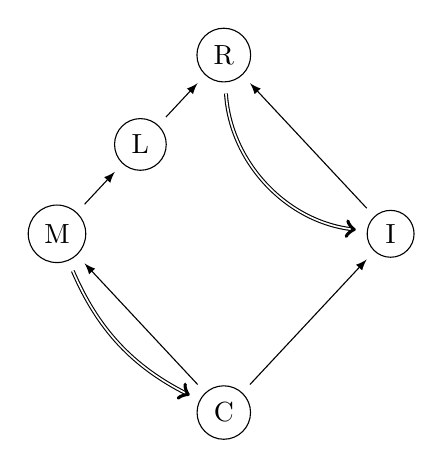
\begin{tikzpicture}[shorten <=0.4em,shorten >=0.4em]
\node [circle,draw,shift={(1ex,15ex)}] (M){M};
\node [circle,draw,shift={(15ex,0ex)}] (C){C};
\node [circle,draw,shift={(29ex,15ex)}] (I){I};
\node [circle,draw,shift={(8ex,22.5ex)}] (L){L};
\node [circle,draw,shift={(15ex,30ex)}] (R){R};
\draw [arrows={-latex}] (I) -- (R);
\draw [arrows={-latex}] (M) -- (L);
\draw [arrows={-latex}] (L) -- (R);
\draw [arrows={-latex}] (C) -- (M);
\draw [arrows={-latex}] (C) -- (I);
\draw[->,double] (M) to[bend right=20] (C);
\draw[->,double](R) to[bend right=40] (I); 
\end{tikzpicture}
\end{Scaled}
\end{minipage}
\begin{minipage}[H]{0.5\textwidth}
\begin{Scaled}{0.6}{0.6}
$
\begin{array}{|l}
\mbox{Nodes:}
\\
\begin{array}{l l}

\begin{tikzpicture}[shorten <=0.4em,shorten >=0.4em]
\node [circle,draw,shift={(0,0)}] (M){M};
\end{tikzpicture}
&\raisebox{1.5ex}{Mutable: alias, write}
\\
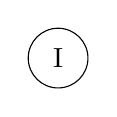
\begin{tikzpicture}[shorten <=0.4em,shorten >=0.4em]
\node [circle,draw,shift={(0,0)}] (I){${\ }$I${\ }$ };
\end{tikzpicture}
&\raisebox{1.5ex}{Immutable: alias, no write}
\\
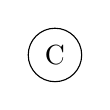
\begin{tikzpicture}[shorten <=0.4em,shorten >=0.4em]
\node [circle,draw,shift={(0,0)}] (C){C};
\end{tikzpicture}
&\parbox{50ex}{Capsule: unique access\\*
Reference used only once}
\\

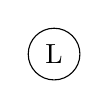
\begin{tikzpicture}[shorten <=0.4em,shorten >=0.4em]
\node [circle,draw,shift={(0,0)}] (L){L};
\end{tikzpicture}
&
\parbox{50ex}{Lent: no alias, write}
\\
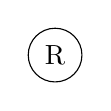
\begin{tikzpicture}[shorten <=0.4em,shorten >=0.4em]
\node [circle,draw,shift={(0,0)}] (C){R};
\end{tikzpicture}
&
\parbox{50ex}{Readable: no alias, no write}
\end{array}
\\
\mbox{Arrows:}
\\
\begin{array}{l l}
\begin{tikzpicture}
\draw [arrows={-latex}] (0,0) -- (1,0);
\end{tikzpicture}
&\mbox{Subtype}
\\
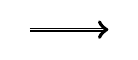
\begin{tikzpicture}
\draw[->,double] (0,0) to (1,0);
\end{tikzpicture}
&\mbox{{Recovery}}
\end{array}
\end{array}
$
\end{Scaled}
\end{minipage}
}
\caption{Type qualifiers and their relationships}
\label{fig:hierarchy}
\end{figure}

\section{Type system}\label{sect:typesystem}
Type contexts are defined by:
\begin{center}
\begin{grammatica}
\produzione{\Delta}{\Gamma;\LentLocked;\StronglyLocked}{type context}\\*
\produzione{\Gamma}{\TypeDec{\T_1}{\x_1},\ldots,\TypeDec{\T_n}{\x_n}}{type assignment}
\end{grammatica}
\end{center} 
{In a type context $\Delta=\Gamma;\LentLocked;\StronglyLocked$, $\Gamma$ is a usual {\em assignment of types} to variables. We write $\dom{\Gamma}$ for the set of variables in $\Gamma$, and  $\SubstFun{\Gamma}{\Gamma'}$ for the concatenation of $\Gamma$ and $\Gamma'$ where, for the variables occurring in both domains, $\Gamma'$ takes precedence.  We will also use $\domMut{\Gamma}$ for the set of mutable variables in $\Gamma$, and other analogous notations.}

{According to our convention, $\LentLocked$ is a sequence $\xs_1\ldots\xs_n$ of sequences of variables, and $\StronglyLocked$ is a sequence of variables. All such sequences are assumed to be sets (that is, order and repetitions are immaterial). The sets  $\xs_1\ldots\xs_n$ are assumed to be pairwise disjoint, and are called \emph{{lent group}s}, whereas the $\mutable$ variables in $\Gamma$ which do not belong to any lent group form the \emph{{mutable group}}. Finally, variables in $\ys$ are called \emph{restricted} variables.}

{Lent groups and restricted variables are the key novelty of our type system.
%, hence we roughly explain their role, which will be formally detailed in the following. 
The property they ensure is that, if $\TypeCheck{\Gamma}{\LentLocked}{\StronglyLocked}{\e}{\T}$, then the final result of $\e$ will be not connected to variables which are in $\LentLocked$ or $\StronglyLocked$. In this way, to ensure that the final result of $\e$ is an isolated portion of store, it is enough to typecheck $\e$ in a type context where all its free mutable variables are in a {lent group} or restricted.  This is a crucial improvement with respect to previous mechanisms of recovery \cite{GordonEtAl12,ClebschEtAl15}, where this could be only ensured if  $\e$ had \emph{only} immutable or isolated ($\capsule$ in our teminology) free variables. 
We have distinct {lent group}s $\xs_1\ldots\xs_n$ since there can be nested recoveries, hence, to ensure that all are safe, we need also the auxiliary property that no aliasing is introduced between different groups, as will be illustrated in detail by the last example of \refToSection{examples}. That is, if the reachable graphs of $\xs_i$ and $\xs_j$ were disjoint before the evaluation of the expression, then after the evaluation they should be still disjoint.\footnote{Note that this is different from \emph{regions} as in, e.g., \cite{BocchinoEtAl09,HallerOdersky10}, which are sets of references \emph{assumed} to be disjoint.}} 

{The type system ensures the above properties by imposing that variables in $\LentLocked$ and $\StronglyLocked$ are used in controlled way:
\begin{itemize}
\item A $\mutable$ variable in $\Gamma$ which belongs to a {lent group} $\xs_i$ can only be used as $\lent$. Notably, write access is not directly allowed since it could introduce aliasing.
\item A $\readable$, $\lent$ or $\mutable$ variable in $\Gamma$ which is restricted cannot be used at all, that is, is hidden.\footnote{{However, we use the terminology ``restricted'' since this hiding is non permanent.}}
\end{itemize}
The important point is that such constraints are not imposed once and for all when typechecking an expression. That is, a subexpression can be typechecked with different {lent group}s and restricted variables, more precisely:
\begin{itemize}
\item In a subexpression we can \emph{swap} one of the {lent group}s $\xs_i$ with the {mutable group}, weakening to $\lent$ the type of the subexpression if it was mutable. 
In this way, write access to variables in $\xs_i$ is allowed, but this is safe since the result of the subexpression is in turn $\lent$, so no aliasing can be introduced with the result of the main expression. 
\item In a subexpression we can \emph{unrestrict} variables in $\ys$, that is, freely use such variables, provided that the type of the subexpression is $\imm$ or $\capsule$.  Again this guarantees that no aliasing can be introduced with the result of the main expression.
\end{itemize} }

Lent groups and restricted variables are introduced as an effect of applying \emph{recovery} rules \rn{t-capsule} and \rn{t-imm}, whereas swapping and unrestricting are obtained by applying rules \rn{{t-swap}} and \rn{t-unrst} rules, as will be explained in detail later. 


Contexts $\Delta=\Gamma;\LentLocked;\StronglyLocked$ are \emph{well-formed}, written $\WellFormedTypeCtx{\Delta}$, 
if, for $\LentLocked=\xs_1\ldots\xs_n$, the following conditions hold:
\begin{itemize}
\item no variable is $\lent$  in $\Gamma$
\item if  $\x\in\xs_i$ for some $i\in 1..n$,  then $\x$ is $\mutable$ in $\Gamma$
\item if $\y\in\StronglyLocked$, then  $\y$ is $\mutable$ or $\readable$  in $\Gamma$
\item if $\y\in\StronglyLocked$ and is $\mutable$ in $\Gamma$, then $\y\in\xs_i$ for some $i\in 1..n$.
%and, for all $\x\in\xs_i$, $\x\in\StronglyLocked$
\end{itemize}
We do not consider $\lent$ variables in $\Gamma$ since assigning the type $\Type{\lent}{\C}$ to a variable $\x$  is encoded by assigning to $\x$ the type $\Type{\mutable}{\C}$ and having $\x$ in a lent group in $\LentLocked$ (see the explanation of rule \rn{t-block} in the following). The  last condition requires \emph{coherency} between $\LentLocked$ and $\StronglyLocked$, that is, restricted mutable variable are in a lent group. It is easy to check that well-formedness of contexts is preserved in type derivations. That is, if $\Delta\TypeCheckGround{\e}{\T}$ and ${\Delta}$ is well-formed, then in all sub-derivations the contexts are well-formed. In the following when we write 
$\Delta\TypeCheckGround{\e}{\T}$ we assume that ${\Delta}$ is well-formed.

In the rules we use information extracted from the class table, which is modelled, as usual, by the following functions:{
\begin{itemize}
\item $\fields{\C}$ gives, for each declared class $\C$, the sequence of its fields declarations
\item {$\method{\C}{\m}$ gives, for each method $\m$ declared in class $\C$, the tuple\\
 $\FourTuple{\T}{\mu}{\Param{\T_1}{\x_1}\ldots\Param{\T_n}{\x_n}}{\e}$ consisting of its return type, type qualifier for $\this$, parameters, and body. }
\end{itemize}
We assume method bodies to be well-typed w.r.t.\ {the type annotations in the method declaration}. More precisely, if
%\begin{quote}
%$\method{\C}{\m}=\FourTuple{\T}{\mu}{\Param{\T_1}{\x_1}\ldots\Param{\T_n}{\x_n}}{\e}$
%\end{quote}
%then $\e$ should be well-typed in a type context where parameters declared $\lent$, including the implicit parameter $\this$, have been encoded by singleton lent groups, expressing the requirement that they should not be aliased by the method. Formally, it should be
%\begin{quote}
%$\TypeCheck{\Gamma}{\{\x_i\mid T_i=\Type{\lent}{\C_i}\}\cup\{\this\mid\mu=\lent\}}{\emptyset}{\e}{\T}$
%\end{quote}
%with $\Gamma=\TypeDec{\Type{\mu'}{\C}}{\this}, \TypeDec{\T'_1}{\x_1},\ldots,\TypeDec{\T'_n}{\x_n}$, where $\T_i=\Type{\mutable}{\C_i}$ if $\T_i=\Type{\lent}{\C_i}$, $\T'_i=\T_i$ otherwise, and $\mu'=\mutable$ if $\mu=\lent$, $\mu'=\mu$ otherwise. 
{\begin{quote}
$\method{\C}{\m}=\FourTuple{\T}{\mu}{\Param{\T_1}{\x_1}\ldots\Param{\T_n}{\x_n}}{\e}$
\end{quote}
then 
\begin{quote}
$\TypeCheck{\Gamma}{\LentLocked}{\emptyset}{\e}{\T}$
\end{quote}
where $\LentLocked$ {consists of} the singletons of the parameters declared $\lent$, including the implicit parameter $\this$, expressing the requirement that they should not be aliased by the method, and $\Gamma=\TypeDec{\Type{\mu'}{\C}}{\this}, \TypeDec{\T'_1}{\x_1},\ldots,\TypeDec{\T'_n}{\x_n}$, where $\T_i=\Type{\mutable}{\C_i}$ if $\T_i=\Type{\lent}{\C_i}$, $\T'_i=\T_i$ otherwise, and $\mu'=\mutable$ if $\mu=\lent$, $\mu'=\mu$ otherwise. 
}

Typing rules are given in \refToFigure{typing}. {In the typing rules, when we need to make explicit the mutable group, we use the  auxiliary judgment $\AuxTypeCheck{\Gamma}{\LentLocked}{\MutGroup}{\StronglyLocked}{\e}{\T}$, which stands for the judgment 
$\TypeCheck{\Gamma}{\LentLocked}{\StronglyLocked}{\e}{\T}$ with the side condition $\MutGroup=\domMut{\Gamma}{\setminus}\LentLocked$, meaning that $\MutGroup$ are the $\mutable$ variables in $\Gamma$ which do not belong to {any lent} group in $\LentLocked$.}

\begin{figure}[ht!]
\framebox{
\begin{footnotesize}
\begin{math}
\begin{array}{l}
\NamedRule{t-capsule}{\AuxTypeCheck{\Gamma}{\LentLocked\ {\xs}}{{\emptyset}}{\StronglyLocked}{\e}{\Type{\mutable}{\C}}}{{\AuxTypeCheck{\Gamma}{\LentLocked}{\MutGroup}{\StronglyLocked}{\e}{\Type{\capsule}{\C}}}}\\
\Space
%{\xs=\domMut{\Gamma}{\setminus}\LentLocked}
\NamedRule{t-imm}{
\AuxTypeCheck{\Gamma}{\LentLocked\ \xs}{{\emptyset}}{\domGeqMut(\Gamma) }{\e}{\Type{\readable}{\C}}
}{
{\AuxTypeCheck{\Gamma}{\LentLocked}{\xs}{\StronglyLocked}{\e}{\Type{\imm}{\C}}}
}{
%{\xs=\domMut{\Gamma}{\setminus}\LentLocked}
}
\\[5ex]
\NamedRule{{t-swap}}{\AuxTypeCheck{\Gamma}{\LentLocked\ \xs'}{\xs}{\StronglyLocked}{\e}{{\T}}}{{\AuxTypeCheck{\Gamma}{\LentLocked\ \xs}{\xs'}{\StronglyLocked}{\e}{{\TPrime}}}}{
%{\xs'=\domMut{\Gamma}{\setminus}(\LentLocked\ \xs)}\\
{\xs\cap\ys}=\emptyset\\
{\TPrime=
\begin{cases}
\Type{\lent}{\C}&\mbox{if}\ \T=\Type{\mutable}{\C}\\
\T&\mbox{otherwise}
\end{cases}}
}
\\[5ex]
\NamedRule{t-{unrst}}{
\TypeCheck{\Gamma}{\LentLocked}{\emptyset}{\e}{{\T}}
}{
\TypeCheck{\Gamma}{\LentLocked}{\StronglyLocked}{\e}{{\T}}
}{{\T=\Type{\mu}{\C}\Longrightarrow\mu\leq\imm}}
\Space
\NamedRule{t-sub}{\TypeCheckShort{\Delta}{\e}{\T}
}{
\TypeCheckShort{\Delta}{\e}{\TPrime}}{
\T\leq\TPrime
}
\\[5ex]
{\NamedRule{t-var}{}{\TypeCheck{\Gamma}{\LentLocked}{\StronglyLocked}{\x}{\TPrime}}{
\Gamma(\x)=\T\ \wedge \ 
\x\notin\StronglyLocked\\
\TPrime=
\begin{cases}
\Type{\lent}{\C}&\mbox{if}\ \T{=}\Type{\mutable}{\C}\,\wedge\,\x\in\LentLocked\\
\T&\mbox{otherwise}
\end{cases}
}}
\\[6ex]
{\NamedRule{t-field-access}{\TypeCheckShort{\Delta}{\e}{\Type{\mu}{\C}}}{\TypeCheckShort{\Delta}{\FieldAccess{\e}{\f_i}}{\TPrime_i}}{
\fields{\C}=\Field{\T_1}{\f_1}\ldots\Field{\T_n}{\f_n}\\
\TPrime_i=\begin{cases}
\Type{\mu}{\C_i}\ \mbox{if}\ \T_i=\Type{\mutable}{\C_i}\\
\T_i\ \mbox{otherwise}
\end{cases}
}}
\\[5ex]
\NamedRule{t-meth-call}{\TypeCheckShort{\Delta}{\e_i}{\T_i}\Space\forall i\in 0..n}{\TypeCheckShort{\Delta}{\MethCall{\e_0}{\m}{\e_1,\ldots,\e_n}}{\T}}{
\begin{array}{l}
\T_0=\Type\mu\C\\
\method{\C}{\m}=\FourTuple{\T}{\mu}{\Param{\T_1}{\x_1}\ldots\Param{\T_n}{\x_n}}{\e}
\end{array}
}
\\[5ex]
\NamedRule{t-field-assign}{
  \TypeCheckShort{\Delta}{\e}{\Type{\mutable}{\C}}
  \Space
  \TypeCheckShort{\Delta}{\e'}{\T_i}
  }{
  \TypeCheckShort{\Delta}{\FieldAssign{\e}{\f_i}{\e'}
  }{\T_i}
  }{
  {\fields{\C}=\Field{\T_1}{\f_1}\ldots\Field{\T_n}{\f_n}}
  }
\\[5ex]
\NamedRule{t-new}{\TypeCheckShort{\Delta}{\e_i}{\T_i}\Space\forall i\in 1..n}{\TypeCheckShort{\Delta}{\ConstrCall{\C}{\e_1,\ldots,\e_n}}{\Type{\mutable}{\C}}}{
\fields{\C}=\Field{\T_1}{\f_1}\ldots\Field{\T_n}{\f_n}\\
}
\\[5ex]
{\NamedRule{t-block}{
{\AuxTypeCheck{\SubstFun{\Gamma}{\TypeEnv{\decs}}}{\LentLocked_i}{\MutGroup_i}{\StronglyLocked'}{\e_i}{\TypeEnv{\decs}(\x_i)}\ \ {\forall i\in 1..n}}\\
\AuxTypeCheck{\SubstFun{\Gamma}{\TypeEnv{\decs}}}{\LentLocked'}{{\MutGroup'}}{\StronglyLocked'}{\e}{\T}}
{\AuxTypeCheck{\Gamma}{\LentLocked}{\MutGroup}{\StronglyLocked}{\Block{\decs}{\e}}{\T}}{
\begin{array}{l}
\decs=\Dec{\T_1}{\x_1}{\e_1}\ldots\Dec{\T_n}{\x_n}{\e_n}\\
\LessEq{(\LentLocked{\setminus}\dom{\decs})}{\LentLocked'}\\
(\MutGroup{\setminus}\dom{\decs})\subseteq\MutGroup'\\
\forall i\in 1..n\ \LentLocked_i\ \MutGroup_i = \LentLocked'\ \MutGroup'\\
\Space \mbox{and}\ \x_i\in\domMut{\TypeEnv{\decs}}\Rightarrow\x_i\in \MutGroup_i\\
\StronglyLocked'={\StronglyLocked}{\setminus}{\dom{\decs}}
\end{array}}}
\end{array}
\end{math}
\end{footnotesize}
}
\caption{Typing rules}\label{fig:typing}
\end{figure}
 
Rules \rn{t-{capsule}} and \rn{t-{imm}} 
 model \emph{recovery},
 that is, can be used to recover a more specific type for an expression,
 under the conditions that the use of some free variables in the expression is} {controlled}.
There are two kinds of recovery:
\begin{itemize}
\item $\mutable\Rightarrow\capsule$
\\* As shown in rule \rn{t-{capsule}}, an expression can be typed $\capsule$ in $\Gamma;\LentLocked;\StronglyLocked$ if it can be typed $\mutable$ by turning in lent the mutable group ($\xs$), which becomes empty.
Formally, this group is added to $\LentLocked$.  
\item $\readable\Rightarrow\imm$ 
\\*As shown in rule \rn{t-{imm}}, an expression can be typed $\imm$ in $\Gamma;\LentLocked;\StronglyLocked$  if it can be typed $\readable$ by {turning in lent the mutable group ($\xs$)}, as in the {recovery} above, and, moreover, restricting currently available mutable, lent, and readable variables ($\domGeqMut(\Gamma)$).
\end{itemize}

Along with {recovery} rules which introduce {lent group}s and restricted variables, we have two corresponding elimination rules.
In the detail:
\begin{itemize}
\item\rn{{t-swap}}
\\* An expression can be typed in $\Gamma;\LentLocked\ \xs;\StronglyLocked$ if it can be typed by turning into mutable 
some {lent group} {($\xs$)}, by swapping this group with the {current mutable group}  ($\xs'$). {The side condition $\xs\cap\ys=\emptyset$ prevents to swap a lent group including restricted variables.}
The type obtained in this way is weakened to $\lent$, if it was $\mutable$.
\item
\rn{t-unrst} 
\\* An expression can be typed in $\Gamma;\LentLocked;\StronglyLocked$ if it can be typed by unrestricting all restricted variables {$\StronglyLocked$}, provided that the type obtained in this way is $\capsule$ or $\imm$ {or a primitive type}.
\end{itemize}

{Note that, without these last two rules, recovery rules would be essentially equivalent to those in prior work \cite{GordonEtAl12,ClebschEtAl15}. Rules \rn{t-swap} and \rn{t-unrst}  add power to the type system, and they are also the reason {it} requires the $\LentLocked$ and $\StronglyLocked$ information during typechecking.
Prior work \cite{GordonEtAl12,ClebschEtAl15} can afford to simply locally using weakening and subtyping to make references inaccessible
or convert $\mutable$ references to $\lent$.}

{Note also that recovery rules, \rn{t-swap}, and \rn{t-unrst}  are not syntax-directed, analogously to the subsumption rule. 
In other words, their functionality does not  restrict how code is written: they are \emph{transparent} to the programmer, in the sense that they are applied when needed.  The programmer can simply rely on the fact that expressions are $\capsule$ or $\imm$, respectively, in situations where this is intuitively expected, as we illustrate by the following examples (other will be provided in next section).}

{We explain now in detail how recovery, swapping and unrestricting work, then comment the other rules.}

\paragraph{Capsule {recovery}} Let us discuss, first, when an expression can be safely typed $\capsule$. {The evaluation of the expression should produce a portion of store which is isolated, apart from external immutable references, formally a right-value where all free variables are immutable. Obviously, this is safe for an expression which has itself no free variables, or where all the free variables are {$\imm$ or $\capsule$}, and, indeed, this was the requirement needed for obtaining {recovery} in previous work \cite{GordonEtAl12}.} However, this requirement is too strong. 
Consider the following sequence of declarations:\label{capsule-example-2}

\begin{lstlisting}
mut D y=new D(0); 
capsule C z={mut D x=new D(y.f); new C(x,x)};  
\end{lstlisting}

The inner block (right-hand side of the declaration of \Q@z@) {can} be typed $\capsule$, even though there is a mutable free variable \Q@y@, since this variable is only used in a field access, hence, intuitively, no aliasing is introduced between \lstinline{y}{} and the final result of the block. 
Indeed, the block reduces\footnote{As formalized in \refToSection{calculus}.} to 
\begin{lstlisting} 
{mut D x=new D(0); new C(x,x)};  
\end{lstlisting}
which is closed.
%, that is, has no free variables. 
To allow such typing, the inner block is {typed} applying rule \rn{t-capsule}, since it can be typechecked $\mutable$ in a type context where variable \lstinline{y}{} is $\lent$. In \refToFigure{TypingOne} we show the type derivation for this example,
{where, for clarity, we always write the mutable group even when it is empty.}
%We use $\deriv$ as a metavariable to denote derivations.
\begin{figure}[t]
\framebox{
\begin{footnotesize}
\begin{math}
\begin{array}{l}
\\
\infer[\scriptstyle{\textsc{(t-capsule)}}]
{\TypeCheck{\Gamma}{\emptyset\ [\texttt{y}]}{\emptyset}{\texttt{\{mut D x=new D(y.f); new C(x,x)\}}}{\Type{\capsule}{\C}}}
{
\infer[\scriptstyle{\textsc{(t-block)}}]
{\TypeCheck{\Gamma}{\texttt{y}\ [\emptyset]}{\emptyset}{\texttt{\{mut D x=new D(y.f); new C(x,x)\}}}{\Type{\mutable}{\C}}}
{
%\infer[\scriptstyle{\textsc{(t-sub)}}]
%{ \TypeCheck{\Gamma'}{\texttt{y}}{\emptyset}{\texttt{new D(y.f)}}{\Type{\lent}{\texttt{D}}}      }
{
\infer[\scriptstyle{\textsc{(t-new)}}]
{\TypeCheck{\Gamma'}{\texttt{y}\ [\texttt{x}]}{\emptyset}{\texttt{new D(y.f)}}{\Type{\mutable}{\texttt{D}}}}
{
\infer[\scriptstyle{\textsc{(t-field-access)}}]
{\TypeCheck{\Gamma'}{\texttt{y}\ [\texttt{x}]}{\emptyset}{\texttt{y.f}}{\intType}}
{
\infer[\scriptstyle{\textsc{(T-var)}}]
{\TypeCheck{\Gamma'}{\texttt{y}\ [\texttt{x}]}{\emptyset}{\texttt{y}}{\Type{\lent}{\texttt{D}}}}{} 
}
}
}
&
\infer[\scriptstyle{\textsc{(T-New)}}]
{\TypeCheck{\Gamma'}{\texttt{y}\ [\texttt{x}]}{\emptyset}{\texttt{new C(x,x)}}{\Type{\mutable}{\texttt{C}}}}
{
\infer[\scriptstyle{\textsc{(T-var)}}]
{\TypeCheck{\Gamma'}{\texttt{y}\ [\texttt{x}]}{\emptyset}{\texttt{x}}{\Type{\mutable}{\texttt{D}}}}
{} 
}
}
}
\\
\\
\Gamma=\texttt{y}{:}\Type{\mutable}{\texttt{D}},\texttt{z}{:}\Type{\capsule}{\texttt{C}}\\
\Gamma'=\SubstFun{\Gamma}{\texttt{x}{:}\Type{\mutable}{\texttt{D}}}=\texttt{y}{:}\Type{\mutable}{\texttt{D}},\texttt{z}{:}\Type{\capsule}{\texttt{C}},\texttt{x}{:}\Type{\mutable}{\texttt{D}}
\end{array}
\end{math}
\end{footnotesize}
}
\caption{Example of type derivation (1)}\label{fig:TypingOne}
\end{figure}

{Note that in an analogous example where the field of class \lstinline{D} has a non primitive type, e.g., \lstinline{String}:}
\begin{lstlisting}
mut D y=new D("hello"); 
capsule C z={mut D x=new D(y.f); new C(x,x)};  
\end{lstlisting}
{the qualifier of the field should be $\imm$, since, otherwise, by introducing a singleton {lent group} \lstinline{y} we would get a $\lent$ type for \lstinline{y.f} as well, see rule \rn{t-field-access}, and a $\lent$ type is not accepted for a constructor argument.}

As a counterexample, consider the following sequence of declarations:
\begin{lstlisting}
mut D y=new D(0); 
capsule C z={mut D x=y; new C(x,x)};  
\end{lstlisting}
Here the inner block cannot be typed $\capsule$, since \Q@y@ is internally aliased. Indeed, the block reduces to \Q@new C(y,y)@ which contains a free mutable variable.
Formally, we cannot apply rule \rn{t-capsule} on the block, since
we should typecheck the block with \Q@y@ in a singleton {lent group}, while the initialization expression of \lstinline{x} should be mutable, see rule \rn{t-block}.

Rule \rn{t-field-assign} requires a mutable type for the receiver.
So, how is it possible to modify (the portion of store denoted by) a $\lent$ reference?
Consider the following simple example:
\begin{lstlisting}
lent D y= new D(0);
y.f=y.f+1;
\end{lstlisting}

This code should be well-typed, since the assignment does not introduce any alias. {To get such typing, we use rule \rn{t-swap} to type the expression
\Q@y.f=y.f+1@. {Indeed, we can} swap the singleton {lent group} \Q@y@ with the empty set.

Moreover, swapping can be applied to achieve {recovery}. Take
the example already considered at page \pageref{capsule-example-1}:
\begin{lstlisting}
mut D y=new D(0); 
capsule C z={mut D x=new D(y.f=y.f+1); new C(x,x)}
\end{lstlisting}
Let $\e$ be the inner block (right-hand side of the declaration of \Q@z@). As in the first example, $\e$ can be typed $\capsule$ if it can be typed \Q@mut@ in a context with type assignment $\texttt{y}{:}\Type{\mutable}{\texttt{D}},\texttt{z}{:}\Type{\capsule}{\texttt{C}}$ and
the {lent group} \Q@y@. However, the assignment \Q@y.f=y.f+1@
is not well-typed in this type context, since the variable \Q@y@ has type \Q@lent D@. However, intuitively, we can see that the assignment does not introduce any alias between \Q@y@ and the final result of $\e$, since it involves only variables which are in the same group (the
singleton \Q@y@), and produces {a result which is not mutable}. {In other words, the result of the evaluation of $\e$ is a capsule, as it has been shown in \refToFigure{esRed2}, so it should be possible to
{type} the expression $\e$ {as} $\capsule$.} 

To {get} such typing, we can apply rule \rn{t-swap} when deriving the type for the subexpression \Q@y.f=y.f+1@, by swapping the group \Q@y@ with the group \Q@x@. 
This ensures that the evaluation of the subexpression typed by this rule will not introduce any alias between the
variables in the swapped group and the mutable group. {The type derivation for the example is given in \refToFigure{TypingTwo}.}
 \begin{figure}[t]
 \framebox{
\begin{footnotesize}
\begin{math}
\begin{array}{l}
\infer[\scriptstyle{\textsc{(t-capsule)}}]
{\TypeCheck{\Gamma}{\emptyset\ [\texttt{y}]}{\emptyset}{\texttt{\{mut D x=new D(y.f=y.f+1); new C(x,x)\}}}{\Type{\capsule}{\texttt{C}}}}
{
\infer[\scriptstyle{\textsc{(t-block)}}]
{\TypeCheck{\Gamma}{\texttt{y}\ [\emptyset]}{\emptyset}{\texttt{\{mut D x=new D(y.f=y.f+1); new C(x,x)\}}}{\Type{\mutable}{\texttt{C}}}
}
{
\infer[\scriptstyle{\textsc{(T-New)}}]
{\TypeCheck{\Gamma'}{\texttt{y}\ [\texttt{x}]}{\emptyset}{\texttt{new C(x,x)}}{\Type{\mutable}{\texttt{C}}}}
{
\infer[\scriptstyle{\textsc{(T-var)}}]
{\TypeCheck{\Gamma'}{\texttt{y}\ [\texttt{x}]}{\emptyset}{\texttt{x}}{\Type{\mutable}{\texttt{D}}}}{}
}
&
\hspace{-1cm}
\infer[\scriptstyle{\textsc{(T-New)}}]
{\TypeCheck{\Gamma'}{\texttt{y}\ [\texttt{x}]}{\emptyset}{\texttt{new D(y.f=y.f+1)}}{\Type{\mutable}{\texttt{D}}}}
{
\infer[\scriptstyle{\textsc{(t-swap)}}]
{\TypeCheck{\Gamma'}{\texttt{y}\ [\texttt{x}]}{\emptyset}{\texttt{y.f=y.f+1}}{\intType}}
{
\infer[\scriptstyle{\textsc{(t-fld-ass)}}]
{\TypeCheck{\Gamma'}{\texttt{x}\ [\texttt{y}]}{\emptyset}{\texttt{y.f=y.f+1}}{\intType}}
{
\infer[\scriptstyle{\textsc{(T-var)}}]
{\TypeCheck{\Gamma'}{\texttt{x}\ [\texttt{y}]}{\emptyset}{\texttt{y}}{\Type{\mutable}{\texttt{D}}}}{}
&
\deduce{\TypeCheck{\Gamma'}{\texttt{x}\ [\texttt{y}]}{\emptyset}{\texttt{y.f+1}}{\intType}}{\vdots}
}
}
}
}
}\\
\\
\Gamma=\texttt{y}{:}\Type{\mutable}{\texttt{D}},\texttt{z}{:}\Type{\capsule}{\texttt{C}}\\
\Gamma'=\SubstFun{\Gamma}{\texttt{x}{:}\Type{\mutable}{\texttt{D}}}=\texttt{y}{:}\Type{\mutable}{\texttt{D}},\texttt{z}{:}\Type{\capsule}{\texttt{C}},\texttt{x}{:}\Type{\mutable}{\texttt{D}}
\end{array}
\end{math}
\end{footnotesize}
}
\caption{Example of type derivation (2)}\label{fig:TypingTwo}
\end{figure}

Note that, when using rule \rn{t-swap} to typecheck a subexpression of an expression {for which we want the capsule or immutability property}, no alias should be introduced between the variables in the group $\xs$ and the result of the expression.  Indeed, in this case the result of the subexpression could contain references to the variables in group $\xs$, which was lent in the original context.To ensure this, the type obtained in this way is weakened to $\lent$, if it was $\mutable$. 
 This is shown by the following example:
\begin{lstlisting}
mut D y=new D(x1,x2);  
mut x1=new A(0); 
mut x2=new A(1);
capsule C z={mut A x=(y.f1=y.f2); new C(x,x)};
\end{lstlisting}
If we apply rule \rn{{t-swap}} when deriving the
type for \Q@y.f1=y.f2@, therefore swapping the group \Q@y@ with \Q@x@, then we derive type
\Q@mut A@, and rule \rn{{t-swap}} would assign type \Q@lent A@ to the expression.
Therefore, the declaration \Q@mut A x=(y.f1=y.f2)@ and the whole expression would be ill-typed.
Indeed, the expression reduces to
\begin{lstlisting}
mut D y=new D(x2,x2);  
mut x1=new A(0); 
mut x2=new A(1);
capsule C z=new C(x2,x2);
\end{lstlisting}
in which the value of \Q@z@ is not a capsule.

\paragraph{{Immutability recovery}} 
{Note that $\capsule$ recovery can only happen for $\mutable$ expressions. In other words, $\mutable$ expressions which reduce to a portion of store with no external mutable references can be safely used where (either a mutable or) an immutable is required. Indeed, every expression which can be typed $\capsule$ can be typed $\imm$ by subtyping. }

{Consider now an expression for which $\capsule$ recovery cannot happen, that is, which can be typed $\lent$ or $\readable$, but cannot be typed $\mutable$, hence should not be used where a $\mutable$ is required. We can \emph{directly}\footnote{That is, not by subtyping.} recover immutability for such an expression, if we can guarantee that the result of the expression will be not connected to external mutable references.   This can be ensured as for the case of $\capsule$ recovery, with one difference. For $\capsule$ recovery, $\lent$ and $\readable$ references can be freely used, since in any case they will be not connected to the final result of the expression. However, if the expression is in turn $\lent$ or $\readable$, its result \emph{could} be connected to $\lent$ or $\readable$ references, hence this should be explicitly prevented by the type system. This is achieved by \emph{restricting} such references, that is, allowing their use only to typecheck subexpressions of $\imm$ $\capsule$ or primitive type.}

Consider the following variant of the first example of capsule {recovery}:
\begin{lstlisting}
mut D y=new D(0); 
imm C z={lent D x=new D(y.f); new C(x,x)};  
\end{lstlisting}
As in the original version, the inner block (right-hand side of the declaration of \lstinline{z}) uses the mutable free variable \lstinline{y} only in a field access, and indeed reduces to the block \Q@{lent D x= new D(0);  new C(x,x)}@ which is closed. However, this block {cannot be typed $\capsule$}, since it cannot be safely assigned to a mutable reference. On the other hand, the block can be safely typed  $\imm$, since, intuitively, it reduces to a portion of store which cannot be modified through any other reference. Formally, the inner block can be {typed $\imm$} by rule \rn{t-imm}, since it can be typechecked $\lent$ in a type context where variable \lstinline{y}{} is in  singleton {lent group} and, moreover, restricted, that is, can be only used to typecheck subexpressions which are $\imm$, $\capsule$, or of a primitive type. 
The type derivation for the example is given in \refToFigure{TypingThree}. 
{Note that, instead of putting \texttt{x} is a sigleton group we could have put \texttt{x} and \texttt{y} in the same 
group in the typing of \lstinline{new C(x,x)}{} and \lstinline{new D(y.f)}{}. That is, replacing}
\verb!{x} {y}! with \verb!{x,y}!  the derivation would still be correct. (Clearly the rule \rn{T-Swap} would swap \verb!{x,y}!
with the empty mutable group.)

\begin{figure}[th]
\framebox{
\begin{footnotesize}
\begin{math}
\begin{array}{l}
\\
\infer[\scriptstyle{\textsc{(t-imm)}}]
{\TypeCheck{\Gamma}{\emptyset\ [\texttt{y}]}{\emptyset}{\texttt{\{lent D x=new D(y.f); new C(x,x)\}}}{\Type{\imm}{\texttt{C}}}}
{
\infer[\scriptstyle{\textsc{(t-block)}}]
{\TypeCheck{\Gamma}{\texttt{y}\ [\emptyset]}{\texttt{y}}{\texttt{\{lent D x=new D(y.f); new C(x,x)\}}}{\Type{\lent}{\texttt{C}}}
}
{
\infer[\scriptstyle{\textsc{(t-new)}}]
{
\TypeCheck{\Gamma'}{\{\texttt{y}\}\ \{\texttt{x}\}\ [\emptyset]}{\texttt{y}}{\texttt{new D(y.f)}}{\Type{\mutable}{\texttt{D}}}
}
{
\infer[\scriptstyle{\textsc{(t-unrst)}}]
{\TypeCheck{\Gamma'}{\{\texttt{y}\}\ \{\texttt{x}\}\ [\emptyset]}{\texttt{y}}{\texttt{y.f}}{\intType}}
{
\infer[\scriptstyle{\textsc{(t-field-access)}}]
{\TypeCheck{\Gamma'}{\{\texttt{y}\}\ \{\texttt{x}\}\ [\emptyset]}{\emptyset}{\texttt{y.f}}{\intType}}
{
\infer[\scriptstyle{\textsc{(T-var)}}]
{\TypeCheck{\Gamma'}{\{\texttt{y}\}\ \{\texttt{x}\}\ [\emptyset]}{\emptyset}{\texttt{y}}{\Type{\lent}{\texttt{D}}}}{} 
}
}
}
&
\infer[\scriptstyle{\textsc{(t-swap)}}]
{\TypeCheck{\Gamma'}{\{\texttt{y}\}\ \{\texttt{x}\}\ [\emptyset]}{\texttt{y}}{\texttt{new C(x,x)}}{\Type{\lent}{\texttt{C}}}}
{
\infer[\scriptstyle{\textsc{(t-new)}}]
{\TypeCheck{\Gamma'}{\texttt{y}\ [\texttt{x}]}{\texttt{y}}{\texttt{new C(x,x)}}{\Type{\mutable}{\texttt{C}}}}
{
\infer[\scriptstyle{\textsc{(T-var)}}]
{\TypeCheck{\Gamma'}{\texttt{y}\ [\texttt{x}]}{\texttt{y}}{\texttt{x}}{\Type{\mutable}{\texttt{D}}}}{}
}
}
}
}
\\  \\
\Gamma=\texttt{y}{:}\Type{\mutable}{\texttt{D}},\texttt{z}{:}\Type{\imm}{\texttt{C}}\\
\Gamma'=\SubstFun{\Gamma}{\texttt{x}{:}\Type{\mutable}{\texttt{D}}}=\texttt{y}{:}\Type{\mutable}{\texttt{D}},\texttt{z}{:}\Type{\imm}{\texttt{C}},\texttt{x}{:}\Type{\mutable}{\texttt{D}}
\end{array}
\end{math}
\end{footnotesize}
}
\caption{Example of type derivation (3)}\label{fig:TypingThree}
\end{figure}

{Restricting $\y$} prevents typechecking examples like the following:
\begin{lstlisting}
mut D y=new D(0); 
imm C z={lent D x=y; new C(x,x)};  
\end{lstlisting}

The significance of the {immutability recovery} is more clearly shown by considering method calls, as will be illustrated in \refToSection{examples}.

\paragraph{Blocks}
{A block $\Block{\decs}{\e}$, where $\decs=\Dec{\T_1}{\x_1}{\e_1}\ldots\Dec{\T_n}{\x_n}{\e_n}$, is well-typed if the right-hand sides of declarations and the body are well-typed, as detailed below.
\begin{itemize}
\item All the expressions are typechecked w.r.t.\ the type assignment $\SubstFun{\Gamma}{\TypeEnv{\decs}}$ where $\TypeEnv{\decs}$  is the same of $\TypeDec{\T_1}{\x_1},\ldots,\TypeDec{\T_n}{\x_n}$, apart that local variables declared $\lent$ have type $\mutable$ (indeed the fact that they are $\lent$ is encoded by  including them in lent groups, see next point).
\item The body is typechecked w.r.t.\ lent groups $\LentLocked'$ and mutable group $\MutGroup'$ which extend those of the enclosing scope, modulo hiding (second and third side conditions). More precisely: variables which are $\mutable$ in $\TypeEnv{\decs}$ can be possibly added to a lent group of the enclosing scope, or can form a new lent group, or can be added to the mutable group $\xs$ of the enclosing scope.
\item The right-hand side of each declaration $\e_i$ is typechecked w.r.t.\ to lent groups $\LentLocked_i$ and mutable group $\xs_i$ obtained from those of the body by swapping $\xs'$ with the group which contains $\x_i$, if $\x_i$ is $\mutable$ in $\TypeEnv{\decs}$ (fourth side condition). Recall that sequences of groups are considered as sets, hence the notation $\LentLocked_i\ \MutGroup_i = \LentLocked'\ \MutGroup'$ means that the two sides are the same set of groups.  This swapping models the fact that the initialization expression of a variable $\x_i$ in a lent group is typechecked considering as mutable group that containing $\x_i$.
For variables in the mutable group, or declared with other modifiers, no swapping is needed.
\item All the expressions are typechecked w.r.t.\ restricted variables which are exactly those of the enclosing scope (modulo hiding).
\end{itemize}
We use the following auxiliary notations.
\begin{itemize}
\item {The {\em type assignment extracted} from a sequence of declarations $\decs$, denoted $\TypeEnv{\decs}$, is defined by: $\TypeEnv{\Dec{\T_1}{\x_1}{\e_1}\ldots\Dec{\T_n}{\x_n}{\e_n}}=\TypeDec{\T'_1}{\x_1},\ldots,\TypeDec{\T'_n}{\x_n}$ where $\T'_i=\Type{\mutable}{\C}$ if  $\T_i=\Type{\lent}{\C}$, $\T'_i=\T_i$ otherwise.}
\item $(\xs_1\ldots\xs_n){\setminus}\xs=(\xs_1{\setminus}\xs)\ldots(\xs_n{\setminus}\xs)$  
\item $\dom{\xs_1\ldots\xs_n}=\{\x\mid \x\in\xs_i\mbox{ for some}\ i\}$
\item $\LessEq{\xs_1\ldots\xs_n}{\ys_1\ldots\ys_m}$ if $\dom{\xs_1\ldots\xs_n}\subseteq\dom{\ys_1\ldots\ys_m}$, and {for all $\x,\y\in\dom{\xs_1\ldots\xs_n}$, $\x,\y\in\xs_i$ if and only if 
$\x,\y\in\ys_j$.}
%\item $\LessEq{\LentLocked}{\LentLocked'}$ if $\dom{\LentLocked}\subseteq\dom{\LentLocked'}$, and {for all $\x,\y\in\dom{\LentLocked}$, $\x\in\xs\in\LentLocked$  and $\y\in\xs\in\LentLocked$ if and only if 
%$\x\in\xs'\in\LentLocked'$ and $\y\in\xs'\in\LentLocked'$.}
%\item $\Extends{\LentLocked}{\zs}{\LentLocked'}$ if $\LessEq{\LentLocked}{\LentLocked'}$ holds, and, moreover, $\dom{\LentLocked'}=\dom{\LentLocked}\cup\zs$.
\end{itemize} }

{Note that local variables declared $\lent$ can be arbitrarily assigned to {lent group}s, to improve expressivity. For instance, it can be necessary to assign a $\lent$ local variable to the same {lent group} {as} some variables of the enclosing scope. This is shown by the following example, where the local variable \lstinline{z1} is used to modify the external reference \lstinline{x}, rather than to construct the block result.}
\begin{lstlisting}
mut D z=new D(0);  
mut C x=new C(z,z);
capsule C y= {
  lent D z1=new D(1); 
  lent D z2=(x.f1=z1);  
  mut D z3 = new D(2);
  new C(z3,z3)
};
\end{lstlisting}
Since 
we need to {recover the capsule property for} the
block on the right-hand side of the declaration of \Q@y@, applying rule \rn{T-capsule} to the block, the context of the typing of such block 
must be \\
{\small $\ \ \ \ {\tt z:\mutable\ D,x:\mutable\ C,y:\capsule\ C; {\{z, x\}}; \emptyset}$}\\
that is, the variables
\Q@z@ and \Q@x@ must be in the same {lent group}. However, assuming that field \lstinline{f1}{} is mutable, to apply rule \rn{t-field-assign} to the expression \Q@x.f1=z1@,  both \Q@x@ and \Q@z1@ have to be mutable. Therefore, we have to apply rule
\rn{t-swap}, and it must be the case that  \Q@x@ and \Q@z1@ are in the same {lent group}. This is possible, with rule \rn{t-block}, by adding \Q@z1@ to the group \verb!{z,x}! in typing the right-hand sides of the declarations and the body.

Note that the following variant of the example, where the result of the block is connected to \lstinline{z1} instead,}
\begin{lstlisting}
mut D z=new D(0);  
mut C x=new C(z,z);
capsule D y= {
  lent D z1=new D(1); 
  lent D z2=(x.f1=z1);  
  new C(z1,z1)
};
\end{lstlisting}
is ill-typed.  Indeed, as before, \Q@z1@ must be in the same group {as} \Q@x@ in order to {recover the $\capsule$ property of} the block, but in this case \Q@z1@ would be $\lent$, hence the whole block.

\paragraph{Other typing rules} 
Other rules are mostly standard, except that they model the expected behaviour of type qualifiers.

{In} rule \rn{t-var}, a variable is weakened to $\lent$ if it belongs to some group in $\LentLocked$, and cannot be used at all if it belongs to $\StronglyLocked$. 

In rule \rn{t-field-access}, in case the field is $\mutable$, the type qualifier of the receiver is propagated to the field. For instance, {mutable} fields referred through a $\lent$ reference are $\lent$ as well. If the field is immutable {(or of a primitive type), instead, then the expression has the field type,} regardless of the receiver type.  

In rule \rn{t-field-assign}, the receiver should be mutable, and the right-hand side must have the field type. Note that this implies the right-hand side to be either $\mutable$ or $\imm$ {(or of a primitive type)}. Hence, neither the left-hand nor the right-hand sides can be $\lent$ or $\readable$. {This prevents the introduction of aliases for such references. However, recall that for $\lent$ references the constraint can be escaped by using, before this rule, rule \rn{t-swap}, at the price of weakening to $\lent$ the type of the expression. }
  
In rule \rn{t-new}, expressions assigned to fields should be either $\mutable$ or $\imm$ (or of a primitive type).  {Again, for $\lent$ references the constraint can be escaped by swapping, getting a $\lent$ expression. }
 Note that an object is created with no restrictions, that is, as $\mutable$.

Finally, note that primitive types are used in the standard way. For instance, in the premise of rule \rn{t-new} the types of constructor arguments could be primitive types, whereas in rule \rn{t-meth-call} the type of receiver could not.  










\section{Programming examples}\label{sect:examples}

In this section we illustrate the {expressivity of the type system by more significant} examples. 
For sake of readability, we use additional constructs, such as {operators of} primitive types, static methods{, private fields,} and while loops. Moreover, we generally omit the
brackets of the outermost block, and abbreviate $\Block{\Dec{\T}{\x}{\e}}{\e'}$ by $\Sequence{\e}{\e'}$ when $\x\not\in\FV{\e'}$, with $\FV{\e}$ the set of the free variables
 of $\e$. 
  
\paragraph{Capsules and swapping}
{The following example illustrates} how a programmer can declare lent references to achieve {recovery}.
The class \Q@CustomerReader@ below models reading information about customers out of a text file formatted as shown in the example:

\begin{lstlisting}
Bob
1 500 2 1300
Mark
42 8 99 100
\end{lstlisting}

In even lines we have customer names, in odd lines we have a shop history: a sequence of product codes.

\begin{lstlisting}
class CustomerReader {
  static capsule Customer readCustomer(lent Scanner s){
      mut Customer c=new Customer(s.nextLine())
      while(s.hasNextNum()){
        c.addShopHistory(s.nextNum())
      }
      return c //ok, capsule recovery
  }
}
\end{lstlisting}
The method \Q@CustomerReader.readCustomer@ takes a \Q@lent Scanner@, assumed to be a class similar to the one in Java,
for reading a file and extracting different kinds of data.
A \Q@Customer@ object is {created reading its name} from the file, and then its shop history is added.
Since the scanner is declared $\lent$, and there are no other parameters, by  {recovery} the result can be declared $\capsule$. {That is, we can statically ensure that the data of the scanner are not mixed with the result.}
Previous work offers cumbersome solutions requiring the programmer to manually handle multiple initialization phases like ``raw'' and ``cooked''~\cite{ZibinEtAl10}.

{The following method \Q@update@ illustrates how we can ``open'' capsules, modify their values and then recover the original \Q@capsule@ guarantee. The} 
method  takes an old customer (as capsule) and a \Q@lent Scanner@ as before.
{%\scriptsize
\begin{lstlisting}
class CustomerReader {...//as before
  static capsule Customer update(capsule Customer old,
                                  lent Scanner s){
    mut Customer c=old//we open the capsule `old'
    while(s.hasNextNum()){
      c.addShopHistory(s.nextNum());
    }recovery
    return c; //ok, capsule recovery
  }
}
\end{lstlisting}
}
Every method {with no} mutable parameters can use the pattern illustrated above: one (or many) capsule parameters are opened  (that is, assigned to mutable local variables) and, in the end, the result is guaranteed to be again a capsule. {This mechanism is not possible in previous work \cite{Almeida97,ClarkeWrigstad03,DietlEtAl07}. The type systems of Gordon et al.~\cite{GordonEtAl12} and Pony \cite{ClebschEtAl15} lack borrowed references in the formalization, but could support the variant where the scanner is isolated ($\capsule$ in our teminology) without losing isolation of the scanner or customer (the
 scanner could remain isolated throughout, relying on their support for dispatching appropriate
 methods on isolated references without explicit unpacking)}.


{In the former example, explicit \capsule\ opening and recovery take place \emph{inside the method body}.
Consider the following alternative version:}
\begin{lstlisting}
class CustomerReader {...//as before
  static mut Customer update(mut Customer c,lent Scanner s){
    while(s.hasNextNum()){
      c.addShopHistory(s.nextNum());
    }
    return c;
  }
}
\end{lstlisting}
{This method {takes now a \mutable\ object and returns} another \mutable\ one, as it usually happens in imperative programming.
Surprisingly enough, this method turns out to be just a more flexible version of the former one. Indeed:
\begin{itemize}
\item If called on \mutable\ data, then it returns \mutable\ data, while a call of the former method was ill-typed.
\item If called on \capsule\ data, then capsule opening implicitly takes place during method call execution, and recovery can be achieved for the method call expression, returning a \capsule\ as for the former method.
\end{itemize}
That is, recovery happens \emph{on the client side}\footnote{{The type systems  of Gordon et al.~\cite{GordonEtAl12} and Pony \cite{ClebschEtAl15} could support a variant analogously to the case above.}}. However, a client does not need to worry about this, and can simply call the method.
In a sense, this version of \Q@update@ is polymorphic: it can be used as either
$\mutable\rightarrow\mutable$ or as $\capsule\rightarrow\capsule$.}

{This pattern can be used in combination with function composition. That is, a chain of $\mutable\rightarrow\mutable$ methods can be called, and, if we start from a \capsule, we will get a \capsule\ in the end.
As shown in our example, these methods can have additional (non \mutable) parameters.}

{Moreover, this method can be trasparently used as $\lent\rightarrow\lent$. That is, if called on  $\lent$ data, then it returns $\lent$ data, by applying rule \rn{t-swap} to the method call expression. Again this can be extended to chains of methods which may have additional (non \mutable) parameters. }

Finally, we show the code of the \Q@Scanner@ itself, and how swapping can be used to update {the
fields of a $\lent$ scanner in a safe way.}

\begin{lstlisting}
class Scanner{
  mut InputStream stream;
  imm String nextLine(mut/*=this qualifier*/){...}
  int nextNum(mut/*=this qualifier*/){...}
  bool hasNextNum(read/*=this qualifier*/){...}
}

lent Scanner s=...
mut InputStream stream1=...
capsule InputStream stream2 = ... 
//s.stream=stream1 //(a)wrong
s.stream=new InputStream("...")//(b)ok, swapping 
s.stream=stream2 //(c)ok, swapping 
\end{lstlisting}

In our type system,  a $\lent$ reference can be regarded as mutable if all the mutable references are regarded as $\lent$, as formally modeled by rule \rn{t-swap}.
% {This mechanism is similar to \emph{viewpoint adaptation}
%as in \cite{DietlEtAl07}. 
This can be trivially applied to line (b), where \Q@s@ is the only free variable, and to  line (c), where the other free variable is declared $\capsule$. 
In line (a), instead, swapping would assign a $\lent$ type to \lstinline{stream1}.

{The $\this$ qualifiers reflect the fact that the first two methods modify, whereas the third only reads, the scanner's state. Note that, as in the previous example, the first two methods can be safely applied to $\lent$ scanners by swapping (in this case the result type, being not mutable, remains the same). Note also that such methods (as any method with no parameters and non mutable result type) could be equivalently have $\this$ qualifier $\lent$, since, intuitively, no aliasing can be introduced for $\this$ (formally, we can apply rule \rn{t-swap} to the method body). On the other hand, the first two methods can be invoked on $\lent$ scanners by by applying rule \rn{t-swap} to the method call expression.}

\paragraph{Readable and immutable references}
We illustrate now the \Q@read@ and \Q@imm@ qualifiers by the example of a \Q@Person@ class with a list of friends.
\begin{lstlisting}
class Person{  
  private mut PersonList friends;  
  read PersonList readFriends (read/*=this qualifier*/) {
    return this.friends;
  }
}
\end{lstlisting}
To give access to the private field, we declare a method {which is like a usual getter, except} that it returns a \Q@read PersonList@ reference. 
In this way, a client can only read the list of friends obtained through an invocation \lstinline{person.readFriends()}{}, with \lstinline{person} of class \lstinline{Person}.
Note that, since the $\this$ qualifier of the method is \lstinline{read}{}, which is the top of the subtyping hierarchy, it can be invoked whichever is the qualifier of \lstinline{person}.
Moreover, in the case \lstinline{person} is \lstinline{imm}, we get an \Q@imm PersonList@ back, by {recovering immutability for the \Q@read@ result}.
Indeed, in this case, we can apply rule \rn{t-imm} to the invocation \lstinline{person.readFriends()}, since the only free variable \Q@person@ is immutable, so no variable needs to be {restricted}.
{This is another case where the method is polymorphic: it can be used as either
$\readable\rightarrow\readable$ or as $\imm\rightarrow\imm$, and a client does not need to worry about, and can simply call the method.}

Assume now that we want, instead, to give permission to a client to modify the list of friends.
In this case, we can declare a getter method with different type annotations:\label{exposer}
\begin{lstlisting}
mut PersonList getFriends(mut/*=this qualifier*/) {
  return this.friends;
}
\end{lstlisting}
This method takes a mutable \Q@Person@ and returns a mutable \Q@PersonList@ reference.
Hence, it cannot be invoked on \Q@read@ or \Q@imm@ objects.
However, this $\mutable$ getter can be invoked on a lent \lstinline{person}{}:
in \Q@person.getFriends()@  the only free variable \Q@person@ can be seen as \Q@mut@.
The result of the method is turned in \Q@lent PersonList@ by the \rn{t-swap} rule {(formally, swapping the singleton {lent} group \Q@person@ with the empty set).}

{Our approach forces the programmer to explicitly choose either $\readable$ or $\mutable$ getters.}
Other works permits the developer to use
either multiple getters or polymorphic type qualifiers, for instance
the type annotation \lstinline{PolyRead} of Javari~\cite{TschantzErnst05} allows one
to keep a single method, providing an additional design choice for programmers.
However, we argue that forcing programmers to consider the two operations as logically different  can be a 
simpler and more explicit programming pattern.
 (In \refToSection{related} we discuss also a third variant, with return type $\lent$.)
%The getter only gives access to the field, so that the data can be read by a client.
%The exposer, instead, gives permission to a client to modify the reachable object graph of the receiver by returning a mutable reference to the field.
In a language supporting many levels of visibility (like protected, package, friend, ...) a programmer may choose a restricted visibility for $\mutable$ getters and a more permissive visibility for $\readable$ getters.
Collection classes also can declare $\readable$ and $\mutable$ getters, as in the following example.
\begin{lstlisting}
class PersonList{...
 void add(mut, mut Person elem){...}
 read Person readElem (read, int index){...}
 mut Person getElem(mut, int index){...}
}
\end{lstlisting}
Finally, we show how we can create mutable objects, mutate them for a while, and then {recover their immutabiity}:
\begin{lstlisting}
class C{
  static mut Person lonelyPersonFactory(){
    return new Person(new PersonList());
  }
  static imm Person happyPersonFactory(){
    mut Person fred=C.lonelyPersonFactory();
    mut Person barney=C.lonelyPersonFactory();
    fred.getFriends().add(barney);
    barney.getFriends().add(fred);
    return fred; //mut Person recovered to be imm 
    //now fred and barney are friends forever!
  }
}
\end{lstlisting}
Here \Q@lonelyPersonFactory()@  creates lonely \Q@Person@s, that have no friends.
However, there is still hope, since they are mutable:
\Q@happyPersonFactory@ creates two lonely people, \Q@fred@ and \Q@barney@, and makes them friends.
Then the function returns \Q@fred@ (and, indirectly, also \Q@barney@ that is now in the reachable object graph of \Q@fred@).
The function body does not use any free variable, so we can {recover the capsule property of} the result, hence return it as \Q@imm@.

\paragraph{Qualifiers are deep} Note that recovery work since qualifiers have a \emph{deep/full} interpretation, in the sense that
they are propagated to the whole reachable object graph. In
a shallow interpretation, instead, it is possible, for instance,
to reach a mutable object from an immutable object. The
advantage of such interpretation is that libraries can declare strong intentions in a coherent and uniform way, independently of the concrete representation of the user input
(that, with the use of interfaces, could be unknown to the
library). On the other side, providing (only) deep/full qualifiers
means that we do not offer any language support for (as an
example) an immutable list of mutable objects.

\paragraph{Nested recovery and groups}
We conclude the section by an example showing that {recoveries} can be nested, {and, to ensure that all are safe, distinct lent groups must be kept.}
Consider the following code, where implementation of \lstinline{A}{} is omitted to emphasize that only type information provided by qualifiers is significant.
%\newpage
\begin{lstlisting}
class A{...
  mut A mix(mut, mut A a){...}
  //inserts a  in the reachable object graph 
    //of the receiver and returns a
  capsule A clone (read){...} 
  //returns a capsule clone of the receiver
  static mut A parse(){...} //reads an A from input
}

mut A a1= A.parse() //outside of recovery
capsule A outerA={//outer recovery
  mut A a2= A.parse()//inside outer recovery
  capsule A nestedA={//nested recovery
    mut A a3= A.parse()//inside nested recovery
    mut A res= ...
    res.mix(a3)
    //this is promoted and assigned to nestedA
  }
  nestedA.mix(a2)
  //this is promoted and assigned to outerA
}
//program continues, using outerA as capsule
\end{lstlisting}

The question is, what can we write instead of the dots, and why.
Clearly, (1) \Q@a3@ is allowed, {since the result of the inner block will be only connected to a local reference}, while
(2) \Q@a1@ and \Q@a2@ are not, since it will be connected to an external mutable reference. 
However, (3) \Q@a1.clone()@ and \Q@a2.clone()@ are allowed, since the method \lstinline{clone} returns a capsule.
In the same way,
(4) \Q@a2.mix(a2).clone()@ is allowed, as well as
 \Q@a1.mix(a1).clone()@.

However, when we start mixing different variables, things become trickier.
 For example, (5) \lstinline{a2.mix(a1).clone()}{} is not well-typed in our type system.
  Indeed, even though, thanks to cloning, mixing \Q@a2@
 and \Q@a1@ does not compromise the capsule well-formedness of \lstinline{nestedA}{} (that is, the nested recovery can be safely applied), the fact that \Q@a2@ and 
 \Q@a1@ are mixed could compromise the capsule well-formedness of \Q@outerA@ when \Q@outerA@ is computed (that is, the outer recovery would be unsafe).

In summary, mixing \Q@a@s {lent groups introduced} for different {recoveries} must be avoided.
Rule \rn{t-swap} swaps one group with another,
thus keeping them distinct.

This last example \label{comparison} illustrates many of the differences w.r.t. {the type system proposed in \cite{GordonEtAl12}, whose notion of \emph{recovery} is less expressive}.
Their system allows (1), and rejects (2) and (5), as ours. However, they conservatively rejects (3) and (4), since 
 the flow is not tracked at a fine enough granularity.
Depending on the concrete application, programmers may need to work around the
limitations of \cite{GordonEtAl12} by reordering local variables,
 introducing stricter type qualifiers or, in general, re-factoring their code.
 However, there may be cases where there is no possible reordering.
\section{Calculus}\label{sect:calculus}
{The calculus has a simplified syntax where we assume that, except from right-hand sides of declarations, subterms of a compound expression are only {values}. This simplification can be easily obtained by a (type-driven) translation of the syntax of \refToFigure{syntax} generating for each subterm {which is not a value} a local declaration of the appropriate type.} 

Simplified syntax and values are defined in \refToFigure{calculus}. 
\begin{figure*}
\framebox{
{\small \begin{grammatica}
\produzione{\e}{\x\mid\FieldAccess{{\val}}{\f}\mid\MethCall{{\val}}{\m}{{\vals}}\mid\FieldAssign{{\val}}{\f}{{\val}}
\mid\ConstrCall{\C}{{\vals}}\mid\Block{\decs}{\val}
}{expression}\\*
\produzione{\dec}{\Dec{\T}{\x}{\e}}{variable declaration}\\*
\\
\produzione{\T}{\Type{\mu}{\C}}{type}\\*
\produzione{\mu}{\mutable\mid\imm\mid\capsule\mid\lent\mid\readable}{type qualifier}\\*
\\
\produzione{{\valPrime,}\val}{{\x\mid\ConstrCall{\C}{\vals}\mid\Block{\dvs}{\val}}}{{value}}\\*
\\
\produzione{\dv}{\Dec{\T}{\x}{\stVal}}{evaluated declaration}\\
%\produzione{{\valPrime,}\val}{{\x\mid\ConstrCall{\C}{\vals}\mid\Block{\dvs}{\val}}}{value}\\*
\produzione{\stVal}{\ConstrCall{\C}{\xs}\mid\Block{\dvs}{\x}\mid\Block{\dvs}{\ConstrCall{\C}{\xs}}}{\storableVal}
%\produzione{\bv}{}{block value}\\
\end{grammatica} }
}
\caption{Simplified syntax and values}\label{fig:calculus}
\end{figure*}
{Syntax of evaluated declarations and right-values from \refToFigure{syntax} is reported for reader's convenience.}

A {\it value} is either a variable (reference), {or a constructor invocation}, or a {value} enclosed in a local store.

{We denote by $\FV{\e}$ the set of the free variables of expression $\e$ (the standard formal definition is in Appendix A).}

We assume the following well-formedness constraints on expressions:
\begin{enumerate}
\item In a block $\Block{\Dec{\T_1}{\x_1}{\e_1}\ldots\Dec{\T_n}{\x_n}{\e_n}}{\val}$, mutual recursion, that is, $\x_j\in\FV{\e_i}$ and $\x_i\in\FV{\e_j}$, is only allowed if both declarations are {evaluated declarations, formally defined in \refToFigure{calculus}}. Hence, as expected, cyclic stores are allowed, such as
\begin{lstlisting}
{mut C y=new C(x); mut C x=new C(y); x}
{mut C x=new C(x); x}
\end{lstlisting}
whereas cyclic expressions such as
\begin{lstlisting}
{mut C y=x.f; mut C x=new C(y); x}, 
{mut C x= x.f; x}
{mut C x=y; mut C y = x; x}
\end{lstlisting}
are ill-formed. Allowing general recursion would require a sophisticated type system, 
as in \cite{ServettoEtAl13}, but this is not the focus of this paper.
\item As already mentioned in \refToSection{typesystem}, variables of $\capsule$ types can occur at most once in their scope. \label{linearity}
This is simply a \emph{syntactic} constraint, that is, we do not 
deal with linear types and the resultant context splitting, or flow-sensitive typing judgments. For instance, the following expression, which clearly
violates the intent of the capsule and immutable qualifiers, is ill-formed:
\begin{lstlisting}
capsule C c= {new C(0)}; 
capsule D d1= {new D(c)}; 
imm D d2 = {new D(c)}; 
...
\end{lstlisting}
Note that a capsule variable is not yet determined to
become mutable or immutable when it is declared, and that determination is made at the time of its unique occurrence.
\end{enumerate}

{Evaluated declarations associate a \emph{right-value} to a variable, which plays the role of a \emph{reference}.
{Hence, they correspond to} the \emph{store} in conventional models of imperative languages.}
%{We recall that a \emph{store} is a sequence $\dvs$ of evaluated declarations, since it plays the role of the store in conventional models of imperative languages. Indeed, each $\dv$ associates a right-}value to a variable, which plays the role of a \emph{reference}. 
In \refToFigure{wellformed} we define {\em {well-formed} right-values and store}. 
\begin{figure}[ht]
\framebox{
\begin{small}
\begin{math}
\begin{array}{c}
\Rule{}{\WFrv{\ConstrCall{\C}{\xs}}}{}\Space\Space
\Rule
{\forall \Dec{\T}{\y}{\stVal}\in\dvs\ \ \WFrv{\stVal}\ }
{{\WFrv{\Block{\dvs}{{\val}}}}}
{\begin{array}{l}
\dvs\neq\epsilon\\
%\cOrx=\x\ \vee\ \cOrx=\ConstrCall{\C}{\xs}\\ 
\dvs=\Reduct{\dvs}{{\FV{{\val}}}}
\end{array}}
%\Rule{\forall \Dec{\T}{\y}{\stVal}\in\dvs\ \ \WFrv{\stVal}\ }{\WFrv{\Block{\dvs}{\x}}}{\begin{array}{l}\dvs\neq\epsilon\\ \dvs=\Reduct{\dvs}{\x}\end{array}}
%\Space\Space\Rule{\forall \Dec{\T}{\y}{\stVal}\in\dvs\ \ \WFrv{\stVal}\ }{\WFrv{\Block{\dvs}{\ConstrCall{\C}{\xs}}}}{\begin{array}{l}\dvs\neq\epsilon\\ \dvs=\Reduct{\dvs}{\xs}\end{array}}\\
\\ \\
\Rule{}{\WFdv{\Dec{\Type{\mu}{\C}}{\x}{\ConstrCall{\C}{\xs}}}}{\mu\neq\capsule}
\Space\Space\Space\Space\Space
\Rule{\WFrv{\Block{\dvs}{{\val}}}\ \ \WFdv{\dvs}}
{\WFdv{\Dec{\Type{\imm}{\C}}{\x}{\Block{\dvs}{{\val}}}}}
{\begin{array}{c}
%\dvs=\Reduct{\dvs}{\y}{\neq\emptyDvs}\\
{\allMut{\dvs}}
\end{array}
}
%\\
%\\
%\Rule{\WFdv{\dvs}}{\WFdv{\Dec{\Type{\imm}{\C}}{\x}{\Block{\dvs}{\ConstrCall{\C}{\xs}}}}}
%{\begin{array}{c}
%%\dvs=\Reduct{\dvs}{\xs}{\neq\emptyDvs}\\
%{\allMut{\dvs}}
%\end{array}
%}
\\ \\
\Rule{\WFdv{\dv}\Space\Space\WFdv{\dvs}}{\WFdv{\dv\ \dvs}}{}
\end{array}
\end{math}
\end{small}
}
\caption{Well-formed right-values and store}\label{fig:wellformed}
\end{figure}

{For a sequence of declarations $\decs=\Dec{\T_1}{\x_1}{\e_1}\ldots\Dec{\T_n}{\x_n}{\e_n}$, and a set of variables $\X$, we write $\connected{\decs}{\X}{\x}$ if $\x$ is (transitively) connected to $\X$ through $\decs$. This relation  is inductively defined as follows:
\begin{center}
$\connected{\decs}{\X}{\x}$ if $\x\in\X$\\
$\connected{\decs}{\X}{\x}$ if $\x\in\FV{\e_i}$, for some $i\in 1..n$, and $\connected{\decs}{\X}{\x_i}$.
\end{center}
The subsequence $\Reduct{\decs}{\X}$ of the declarations that are (transitively) used by $\X$ is defined by: for all $i\in 1..n$, $\Dec{\T_i}{\x_i}{\e_i}\in\Reduct{\decs}{\X}$ if  $\connected{\decs}{\X}{\x_i}$.
}
\\
We write $\allMut{\dvs}$ if, for each $\Dec{\Type{\mu}{\C}}{\x}{{\stVal}}\in\dvs$, $\mu\geq\mutable$, and $\allImm{\dvs}$ if, for each $\Dec{\Type{\mu}{\C}}{\x}{{\stVal}}\in\dvs$, $\mu=\imm$. 

Rules in the first line define well-formed right-values. 
They state that a right-value should not contain garbage and useless blocks, and that, in case it is a block, 
{the right-hand sides of declarations are, in turn, well-formed right-values.}

Rules in the second and third line define {well-formed}  evaluated declarations or stores. The first rule {states} that
a right-value which is an object state can be associated to any reference which is not $\capsule$.
The second rule {states} that a right-value which is a block can only be associated to an $\imm$ reference,
its local store should not contain $\imm$ references, and, in addition to be a well-formed
right-value, the block should contain a well-formed local store.    
The last rule states that a (non empty) sequence of evaluated declarations is a well-formed store if each one is a well-formed. 

These rules {altogether} imply that in a well-formed store:
\begin{itemize}
\item There are no $\capsule$ references. Indeed, $\capsule$ declarations are ``temporary'', that is, are expected to be consumed as soon as their right-hand side has been evaluated, as will be formalized by reduction rule \rn{capsule-elim} in \refToFigure{reduction}.
\item  There are at most \emph{two} levels, that is, the right-value of an $\imm$ reference can contain in turn a local store of non $\imm$ references. Indeed, additional levels can safely be ``flattened'', as will be formalized by reduction rules \rn{mut-move} and \rn{imm-move} in \refToFigure{reduction}.
\end{itemize}
For instance, assuming that class \lstinline{C} has two $\mutable$  fields of class \lstinline{D} and one $\imm$ of class \lstinline{C}{}, and class  \lstinline{D} has an integer field, the following is a store:
\begin{small}
\begin{lstlisting}
mut D x = new D(0);
imm D y = new D(1);
imm C z = { 
  mut D x = new D(0);
  mut D y = new D(1);
  new C(x,y,z) 
  };
\end{lstlisting}
\end{small}
Note that mutable variables in the local store of \lstinline{z}{} are not visible from the outside. 
This models in a natural way the fact that the portion of store denoted by  \lstinline{z}{} is indeed immutable

Expressions are equivalent modulo the congruence $\cong$ defined by the rules of \refToFigure{congruence}. 
\begin{center}
\begin{figure}[ht]
\framebox{
\begin{small}
\begin{math}
\begin{array}{l}
\\
\Space\Space\Space{\NamedRuleOL{alpha}{\congruence{\Block{\decs\ \Dec{\T}{\x}{\e}\ \decs'}{\val}}{{\Block{\Subst{\decs}{\y}{\x}\ \Dec{\T}{\y}{\Subst{\e}{\y}{\x}}\ \Subst{\decs'}{\y}{\x}}{\Subst{\val}{\y}{\x}}}}}{}}\Space\Space\Space
\\ \\
\Space\Space\Space\Space\Space\NamedRuleOL{reorder}{\congruence{
\Block{
\decs\ {\dv}\ \decs'
}{\val}
}{
\Block{
{\dv}\ \decs\ \decs'\ 
}{\val}
} }{}\Space\Space\Space
\\
\end{array}
\end{math}
\end{small}
}
\caption{Congruence on expressions}
\label{fig:congruence}
\end{figure}
\end{center}
Rule \rn{alpha} is the usual $\alpha$-conversion. We write $\Subst{\e}{\e'}{\x}$
for the expression obtained by replacing all (free)
occurrences of $\x$ in $\e$ by $\e'$ {(the standard formal definition is in the Appendix)}. The condition $\x,\y\not\in\dom{\decs\,\decs'}$ is implicit by well-formedness of blocks. Rule \rn{reorder} states that we can move evaluated declarations in an arbitrary order.  
On the other hand, $\decs$ and $\decs'$ cannot be swapped, since this could change 
the order of side effects. 

Values are equivalent modulo the congruence $\cong$ defined by the rules of \refToFigure{congruenceVal}. 
\begin{figure}[ht]
\framebox{
\begin{small}
\begin{math}
\begin{array}{l}
\NamedRuleOL{new}
{
\begin{array}{l}
{\ConstrCall{\C}{
  \val_1,.., \val_{i-1},\val_i,\val_{i+1},..,\val_n}}\\
  \cong{\Block{\Dec{\T_i}{\x}{{\val_i}}}{\ConstrCall{\C}{\val_1,.., \val_{i-1},\x,\val_{i+1},..,\val_n}}}
\end{array}
}
{\begin{array}{l}
\fields{\C}{=}\Field{\T_1}{\f_1}..\Field{\T_n}{\f_n}\\
\notRef{\val_i}\\
\x\not\in\FV{\val_j}\ \ (1\leq j\leq n)
\end{array}}
\\[3ex]
\NamedRuleOL{body}{\congruence{\Block{\dvs}{\Block{\dvs'\ \dvs''}{\val}}}{\Block{\dvs\ \dvs'}{\Block{\dvs''}{\val}}}}
{\begin{array}{l}
{\noCapture{\dvs}{\dom{\dvs'}}}\\
%\FV{\dvs'}\cap\dom{\dvs}=\emptyset\\
{\noCapture{\dvs'}{\dom{\dvs''}}}
%\FV{\dvs}\cap\dom{\decs}=\emptyset
\end{array}
}
\\[3ex]
{\NamedRuleOL{garbage}{\congruence{\Block{\dvs\ \dvs' }{\val}}{\Block{\dvs'}{{\val}}}}
{\noCapture{\Block{\dvs'}{\val}}{\dom{\dvs}}}}
%\FV{\Block{\decs}{\val}}\cap\dom{\dvs}=\emptyset}
\\[3ex]
\NamedRuleOL{block-elim}{\congruence{\Block{}{{\val}}}{\val}}{}
\end{array}
\end{math}
\end{small}
}
\caption{Congruence on values}
\label{fig:congruenceVal}
\end{figure}
By rule \rn{new} we can assume that arguments of a constructor invocation are references, by introducing local declarations of the appropriate type. The notation $\notRef{\val}$ means that $\val$ is not a variable. 
The following three rules deal with block values.
By rule \rn{body} we can move a sequence of evaluated declarations
from a block to the directly enclosing block, and conversely. The notation $\noCapture{\e}{\xs}$ means that free variables in $\e$ are not captured by $\xs$, formally: $\FV{\e}\cap\xs=\emptyset$, and analogously for $\noCapture{\dvs}{\xs}$. 
The two side conditions ensure that moving the declarations {$\dvs'$} does not cause either scope extrusion 
or capture of free variables. More precisely: the first condition prevents capturing with $\dvs'$ some free 
variables of the enclosing block, whereas the second prevents moving outside a declaration in $\dvs'$ which 
depends on local variables of the inner block (declared in $\dvs''$). The first side condition can be 
satisfied by $\alpha$-conversion of the inner block, whereas the second cannot. 
By rule \rn{garbage} we can remove useless local store from a block.
Finally, rule \rn{block-elim} states the obvious fact that a block with no declarations is equivalent 
to its body.

{Congruence preserves types. We have to assume that the congruent expressions be typable, since rule
\rn{garbage} eliminates declarations from blocks that without this assumption could be not typable.
\begin{proposition}\label{lemma:congruenceTypes}
Let $\TypeCheck{\Gamma}{\LentLocked}{\StronglyLocked}{\e}{{\T}}$. If $\e\cong\e'$ and for some $\Gamma'$, $\LentLocked'$, $\StronglyLocked'$ and $\T'$ we have  that $\TypeCheck{\Gamma'}{\LentLocked'}{\StronglyLocked'}{\e'}{{\T'}}$, then $\TypeCheck{\Gamma}{\LentLocked}{\StronglyLocked}{\e'}{{\T}}$
\end{proposition}
\begin{proof}
By cases on the congruence rule used. \qed
\end{proof}}

Let a {\em  well-formed value} be either a variable or a well-formed right-value.
We can show that any value is congruent to a well-formed value.
\begin{proposition}\label{lemma:congruenceValue}
Let $\val$ be a value, then either $\congruence{\val}{\x}$ for some variable $\x$, or $\congruence{\val}{\stVal}$ for some 
\storableVal\  $\stVal$ {such that $\WFrv{\stVal}$}. 
\end{proposition}
\begin{proof}
By induction on values using the congruence rule of \refToFigure{congruenceVal}.\qed
\end{proof}

The reduction relation is defined by the rules in \refToFigure{reduction}, where $\ctx$ is an {\em evaluation context} 
defined by:
\begin{center}
$\ctx ::=\emptyctx\mid\Block{\dvs\ \Dec{\T}{\x}{\ctx}\ \decs}{\val}
$
\end{center}
{In this definition, and in the following we assume that the metavariables $\val$, $\stVal$, $\dv$ and $\dvs$ denote values,  right-values, evaluated declarations, and stores which are well-formed. The assumption on $\val$ and $\stVal$ can be achieved by Proposition~\ref{lemma:congruenceValue}.}

To lighten notations, here and in what follows we sometimes use the wildcard $\_$ when a metavariable 
is not significant.

\begin{figure}[ht]
\framebox{
\begin{small}
\begin{math}
\begin{array}{l}
%\NamedRule{ctx}{\reduce{\e}{\e'}}{\reduce{\Ctx{\e}}{\Ctx{\e'}}}{}
%\Space
\NamedRuleOL{field-access}{\reduce{\Ctx{\FieldAccess{{\val}}{\f}}}
{\Ctx{\extractField{\ctx}{\val}{i}}}}{
\begin{array}{l}
{\extractType{\ctx}{\val}=\Type{\mu}{\C}}\\
\fields{\C}=\Field{\T_1}{\f_1}\ldots\Field{\T_n}{\f_n}\ \mbox{and}\  \f=\f_i
%\\ \mu=\imm\implies\isCapsule{\ctx}{\val}
\end{array}
}
\\[4ex]
\NamedRuleOL{invk}
{
\begin{array}{l}
\Ctx{\MethCall{\val}{\m}{\val_1,\ldots,\val_n}}\\
\longrightarrow
\Ctx{
\Block{
\Dec{\Type{\mu}{\C}}{\,\this}{\val}\
\Dec{\T_1}{\x_1}{\val_1}
\ldots
\Dec{\T_n}{\x_n}{\val_n}\
\Dec{\T}{\z}{\e}
}{\z}
}
\end{array}
}
{
\begin{array}{l}
{\extractType{\ctx}{\val}=\Type{\_}{\C}}\\
\method{\C}{\m}=\\
\Space \FourTuple{\T}{\mu}{\Param{\T_1}{\x_1}\ldots\Param{\T_n}{\x_n}}{\e}
\end{array}
}
\\[4ex]
{\NamedRuleOL{field-assign-prop}{\reduce{\Ctx{\FieldAssign{{\val}}{\f}{\valPrime}}}{\Ctx{\Block{\Dec{\Type{\mu}{\C}}{\x}{{\val}}\
\Dec{\T_i}{\z}{(\FieldAssign{\x}{\f}{\valPrime})}}{\z}}}}
{
\begin{array}{l}
{\notRef{\val}}, 
\typeOf{\val}=\Type{\mu}{\C}\\
\fields{\C}=\Field{\T_1}{\f_1}\ldots\Field{\T_n}{\f_n}\\
\f=\f_i
\end{array}
}}
\\[4ex]
\NamedRuleOL{field-assign}{
\begin{array}{l}
{
\Ctx{\Block{\dvs\ \Dec{\T}{\z}{\CtxP{\FieldAssign{\x}{\f}{{\valPrime}}}}\ \decs}{\val}}
}\\
\longrightarrow
{
\Ctx{\Block{{\Update{\dvs}{\x}{i}{{\valPrime}}}\ \Dec{\T}{\z}{\CtxP{{\valPrime}}}\ \decs}{\val}}
}
\end{array}
}
{
\begin{array}{l}
\dvs(\x)=\Dec{\mu}{\x}{\ConstrCall{\C}{\_}},{\mu\geq\mutable}\\
{\noCapture{\x}{\HB{\ctxP}},\noCapture{\valPrime}{\HB{\ctxP}}}\\
%(\{\x\}\cup\FV{\valPrime})\cap\HB{\ctx}=\emptyset}\\
\fields{\C}=\Field{\T_1}{\f_1}\ldots\Field{\T_n}{\f_n}\ \mbox{and}\  \f=\f_i
\end{array}
}
\\[4ex]
\NamedRuleOL{field-assign-move}
{
\begin{array}{l}
\Ctx{\Block
	{\dvs'\
		\Dec{\T'}{\z'}
		{\Block
			{\dvs\
			\Dec{\T}{\z}
			{\CtxP{\x.\f{=}{\valPrime}}
			}\
			\decs
			}
			{\val}
		}\
		\decs'
	}
	{\val'}}\\
{\longrightarrow}
	\Ctx{\Block{\dvs'\
		\dvs\
		\Dec{\T'}{\z'}
		{
		\Block{
			\Dec{\T}{\z}
			{\CtxP{\x.\f{=}{\valPrime}}
			}\
			\decs
		}
		{\val}
		}\ 
		\decs'
	}
	{\val'}	}
\end{array}
}{
\begin{array}{l}
\hspace{-.2cm}\FV{\valPrime}{\cap}\dom{\dvs}{=}\xs{\neq}\emptyset\\
\hspace{-.2cm}\noCapture{\x}{\HB{\ctxP}\cup\dom{\dvs}}\\
\hspace{-.2cm}\noCapture{\valPrime}{\HB{\ctxP}}\\
\hspace{-.2cm}{\noCapture{\Block{\dvs'\ \decs'}{\val'}}{\dom{\dvs}}}\\
\hspace{-.2cm}{\Reduct{(\dvs\ \decs)}{{\xs}}=\dvs}
\end{array}
}
\\[4ex]
\NamedRuleOL{alias-elim}{\reduce{\Ctx{\Block{\dvs\ \Dec{\T}{\x}{\y}\ \decs }{\val}}}{\Ctx{\Subst{\Block{\dvs\ \decs}{\val}}{\y}{\x}}}}
{}
\\[4ex]
\NamedRuleOL{capsule-elim}{
\begin{array}{l}
{\Ctx{\Block{\dvs\ \Dec{\Type{\capsule}
{\C}}{\x}{{\val}}\ \decs }{\val'}}}
\\ \longrightarrow
{\Ctx{\Subst{\Block{\dvs\ \decs}{\val'}}{{\val}}{\x}}}
\end{array}
}
{%\isCapsule{\Ctx{\Block{\dvs\ \Dec{\Type{\capsule}{\C}}{\x}{{\emptyctx}}\ \decs }{\val'}}}{{\val}}
}
\\[4ex]
%\NamedRuleOL{imm-right}{
%\begin{array}{l}
%\Ctx{\Block{\dvs'\ \Dec{\Type{\imm}{\C}}{\x}{\Block{\dvs}{\y}}\ \decs}{\val}}
%\\ \longrightarrow
%
%\Ctx{\Block{\dvs'\ \Dec{\Type{\imm}{\C}}{\x}{\Block{\dvs}{{\ConstrCall{\D}{\xs}}}}\ \decs}{\val}}
%\end{array}
%}
%{\dvs(\y)=\Dec{\T}{\y}{\ConstrCall{\D}{\xs}}}
%\\[4ex]
\NamedRuleOL{mut-move}{
\begin{array}{l}
{
\Ctx{\Block{\dvs'\ \Dec{\Type{\mu}{\C}}{\x}{\Block{\dvs\ \dvs''}{\val}}\ \decs'}{\val'}}
}
\\ \longrightarrow
{
\Ctx{\Block{\dvs'\ \dvs\ \Dec{\Type{\mu}{\C}}{\x}{\Block{\dvs''}{\val}}\ \decs'}{\val'}}
}
\end{array}
}{\begin{array}{l}
\mu \geq \mutable\\
{\noCapture{\Block{\dvs'\ \decs'}{\val'}}{\dom{\dvs}}}\\
%\FV{\Block{\dvs'\ \decs'}{\val'}}\cap\dom{\dvs}=\emptyset\\
{\noCapture{\dvs}{\dom{\dvs''}}}
%\FV{\dvs}\cap\dom{\decs}=\emptyset
\end{array}}
\\[4ex]
\NamedRuleOL{imm-move}{
\begin{array}{l}
{
\Ctx{\Block{\dvs'\ \Dec{\Type{\mu}{\C}}{\x}{\Block{\dvs\ \dvs''}{\val}}\ \decs'}{\val'}}
}
\\ \longrightarrow
{
\Ctx{\Block{\dvs'\ \dvs\ \Dec{\Type{\mu}{\C}}{\x}{\Block{\dvs''}{\val}}\ \decs'}{\val'}}
}
\end{array}
}{\begin{array}{l}
\mu \leq \imm, {\allImm{\dvs}}\\
%\extractMod{\dv}=\imm\ \forall \dv\in\dvs\\
{\noCapture{\Block{\dvs'\ \decs'}{\val'}}{\dom{\dvs}}}\\
%\FV{\Block{\dvs'\ \decs'}{\val'}}\cap\dom{\dvs}=\emptyset\\
{\noCapture{\dvs}{\dom{\dvs''}}}
%\FV{\dvs}\cap\dom{\decs}=\emptyset
\end{array}}
\end{array}
\end{math}
\end{small}
}
\caption{Reduction rules}
\label{fig:reduction}
\end{figure}
In rule \rn{field-access}, the type $\Type{\mu}{\C}$ of the receiver $\val$ in the context is found, fields of the class $\C$ are retrieved from the class table, it is checked that $\f$ is actually the name of a field of $\C$, say, the $i$-th field, and the field access is reduced to the $i$-th field of the receiver.
%If the qualifier $\mu$ is $\imm$, then it is checked that the receiver is a $\capsule$. 
%\MSComm{it seams disaligned with the rule, where there is no capsule checking}
%The judgment $\isCapsule{\ctx}{\val}$ holds if, for all $\x\in\FV{\val}$, {$\extractDec{\ctx}{\x}=\Dec{\Type{\imm}{\_}}{\x}{\_}$}

The auxiliary functions $\aux{type}$ and $\aux{get}$ extract the type, and the $i$-th field, respectively, of a value in a context (only needed when the value is a reference). In the definitions, by Proposition~\ref{lemma:congruenceValue}, we assume that values are either references or \storableVals.
{\begin{small}
\begin{quote}
$\extractType{\ctx}{\x}=\T$ if $\extractDec{\ctx}{\x}=\Dec{\T}{\x}{{\_}}$ \\
$\extractType{\ctx}{\stVal}=\typeOf{\stVal}$\\
$\typeOf{\ConstrCall{\C}{\xs}}=\typeOf{\Block{\dvs}{\ConstrCall{\C}{\xs}}}=\Type{\mutable}{\C}$\\
$\typeOf{\Block{\dvs}{\x}}=\T$ if $\dvs(\x)=\Dec{\T}{\x}{{\_}}$\\
\\
$\extractField{\ctx}{\x}{i}=\fieldOf{{\stVal}}{i}$ if $\extractDec{\ctx}{\x}=\Dec{\_}{\x}{{\stVal}}$\\
$\extractField{\ctx}{\stVal}{i}=\fieldOf{\stVal}{i}$\\
{$\fieldOf{\ConstrCall{\C}{\x_1,\ldots,\x_n}}{i}=\x_i$}\\
{$\fieldOf{\Block{\dvs}{\ConstrCall{\C}{\x_1,\ldots,\x_n}}}{i}=\Block{\dvs}{\x_i}$}\\
{$\fieldOf{\Block{\dvs}{\x}}{i}=\Block{\dvs}{\val}$ if $\dvs(\x)=\Dec{\_}{\x}{\stVal}$ and $\fieldOf{\stVal}{i}=\val$}
\\
$\extractDec{\Block{\dvs\ \Dec{\T}{\_}{\ctx}\ \decs}{\val}}{\x}=\begin{cases}
\extractDec{\ctx}{\x}&\mbox{if}\ \extractDec{\ctx}{\x}\ \mbox{defined, otherwise}\\
\dvs(\x)&\mbox{if}\ \dvs(\x)\ \mbox{defined}
\end{cases}$
\end{quote}
\end{small}}
Note that a field access $\FieldAccess{\x}{\f}$, if $\x$ has qualifier $\geq\mutable$,  always returns a reference, since the right-value of $\x$ is necessarily an object state.
If $\x$ is immutable, instead, the field access could return a (copy of) the value stored in the field. This duplication preserves the expected semantics in the case of an immutable reference $\x$, whereas it would be wrong for a mutable reference, since a modification of the object denoted by $\x$ is expected to affect $\FieldAccess{\x}{\f}$ as well, and conversely.

For instance, given the value:
\begin{quote}
$\val=$
\Q@{mut C x=new C(x,y,z); mut D y=new D(0); new C(x,y,z) }@
\end{quote}
we have:
\begin{enumerate}
\item $\fieldOf{\val}{1}=$
\Q@{mut C x=new C(x,y,z); mut D y=new D(0); x }@
\item $\fieldOf{\val}{2}=$
\Q@{mut C x=new C(x,y,z); mut D y=new D(0); y}@
\item $\fieldOf{\val}{3}=$
\Q@{mut C x=new C(x,y,z); mut D y=new D(0); z}@
\end{enumerate}
where 1 is a well-formed value, 2 is congruent by rule \rn{garbage} to the  well-formed value
\Q@{mut D y=new D(0)   y}@, and 3 is congruent by rules \rn{garbage} and \rn{block-elim}, to the well-formed value \Q@z@.

If the value $\val$ above is the right-value of a reference, then such reference is necessarily $\imm$. In this case, $\val$ 
was expected to be a capsule, the variable $\z$ should be declared $\imm$ in the enclosing context.


In rule \rn{invk}, the class $\C$ of the receiver $\val$ is found, and method $\m$ of $\C$ is retrieved from the class table. The call is reduced to a block where declarations of the appropriate type for $\this$, the parameters, and the result are initialized with the receiver, the arguments, and the method body, respectively. The last declaration, variable $\z$, is
 needed to preserve the simplified syntax.

Rule \rn{field-assign-prop} handles the case of a field assignment where the receiver is not a reference (denoted $\notRef{\val}$). In this case, a local reference initialized with the receiver is introduced, and the field access is propagated to such reference. 

In rule \rn{field-assign}, given a field assignment where the receiver is a reference $\x$, the first enclosing declaration for $\x$ is found (the side condition {$\noCapture{\x}{\HB{\ctxP}}$} ensures that it is actually the first), it is checked that the qualifier of the type of $\x$ is $\geq\mutable$, and fields of the class $\C$ of $\x$ are retrieved from the class table. If $\f$ is the name of a field of $\C$, say, the $i$-th, then the $i$-th field of the right-value of $\x$ is updated to $\valPrime$, which is also the result of the field assignment. 
We write $\HB{\ctx}$ for the \emph{hole binders} of $\ctx$, that is, the variables declared in blocks enclosing the
context hole (the standard formal definition is in the Appendix) and $\Update{\dvs}{\x}{i}{{\valPrime}}$ for the sequence of evaluated declarations obtained from $\dvs$ by replacing the $i$-th field of the right-value of $\x$ with ${\valPrime}$ (the obvious formal definition is omitted).

The side condition {$\noCapture{\valPrime}{\HB{\ctxP}}$}, requiring that there are no inner declarations for some free variable in $\valPrime$, prevents scope extrusion. For instance, without this side condition, the term

\begin{small}
\begin{lstlisting}
mut C x= new C(...);
imm C z= { 
  mut D y1= new D(0);
  mut D y2= ( x.f = y1);
  mut D y3= new D(1);
  new C(y3) };
x
\end{lstlisting}
\end{small}

would erroneously reduce to 

\begin{small}
\begin{lstlisting}
mut C x= new C(y1); 
imm C z= { 
  mut D y = new D(0);
  mut D y2= y1;
  mut D y3= new D(1);
  new C(y3) };
x
\end{lstlisting}
\end{small}
Thanks to the side condition, instead, rule \rn{field-assign} is not applicable. However, 
rule \rn{field-assign-move} can be applied.

Rule \rn{field-assign-move} moves store out of a block when this is needed to safely perform field-assignment (that is, to avoid scope extrusion).
In this rule,  given a field assignment of shape $\FieldAssign{\x}{\f}{\valPrime}$, the first enclosing block containing (evaluated) declarations for some free variables $\xs$  of $\valPrime$ is found (the side condition {$\noCapture{\valPrime}{\HB{\ctxP}}$} ensures that it is actually the first). If a declaration for $\x$ can only be found in an outer scope (side condition {$\noCapture{\x}{\HB{\ctxP}\cup\dom{\dvs}}$}), then the store formed by the $\xs$ references, together with all the other references they (recursively) depend on (last side condition) is moved to the directly enclosing block.

For the example above, by applying rule \rn{field-assign-move} we get:

\begin{small}
\begin{lstlisting}
mut C x = new C(...)  
mut D y1 = new D(0)
imm C z = { 
  mut D y2 = ( x.f = y1)
  mut D y3 = new D(1)
  new C(y3) }  
x
\end{lstlisting}
\end{small}
Now, rule \rn{field-assign} can be safely applied to the term.
In general, we may need to apply rule \rn{field-assign-move} many times before reaching the declaration of $\x$. 


The remaining rules handle blocks.

The first two rules eliminate a single declaration of shape $\Dec{\T}{\x}{\val}$ which is \emph{not} well-formed store. 

 In rule \rn{alias-elim}, a reference $\x$ which is initialized as an alias\footnote{{An analogous rule would handle variables of primitive types in an extension of the calculus including such types.}} of another reference $\y$ is eliminated by replacing all its occurrences.
 
In rule \rn{capsule-elim}, a $\capsule$ reference $\x$ is eliminated by replacing the occurrence of $\x$ (unique by the well-formedness constraint) by its value. %, which is checked to be a capsule.
Note that, in rule \rn{alias-elim}, $\y$ cannot be a $\capsule$ reference (since we would have applied rule \rn{capsule-elim} before), hence  duplication of $\capsule$ references cannot be introduced{, and well-formedness is preserved.} 

Rule \rn{mut-move} moves store out of a block associated to a {reference with qualifier $\geq\mutable$}. 
This is always safe, provided that no variables of the outer scope are captured (second side condition, which can be obtained by $\alpha$-renaming), and that the moved declarations do not refer to other declarations of the inner block (last side condition). 

Rule \rn{imm-move} moves store out of a block associated to a {reference with qualifier $\leq\imm$}. In this case, this is only safe for a store of $\imm$ references. The same side conditions of the previous rule are needed.










\section{Results}
\label {Sec:Results}

We present our results for each of the three research questions posed in the introduction. In most cases we found similar trends in Tanzania and Kenya so we report merged findings. We highlight areas where we observed different trends in the two countries. While we often provide the number of responses corresponding to a particular code to give readers a sense of the frequency of each theme in our interviews, we caution that this is a qualitative study and these numbers should not be interpreted as representative of frequencies of beliefs and behaviors in the population.  
\begin {table} [htbp]
\caption{A summary of workarounds by users and agents}
\centering
\begin {tabular} {|p{3cm}|p{2.7cm}|p{1.8cm}|}
\hline
\multicolumn{2}{|l|}{\textbf{Transaction Execution Workarounds}}& \textbf{Changing Component}\\
\hline
\multirow[c]{2}{*}{\textbf{Alternative execution}}& Agent executes transfer& Agent \\ \cline{2-3} & Transact at a distance & User \& Agent\\
\hline
\multirow[c]{2}{*}{\textbf{Alternative services}}& Advance transactions& \multirow[c]{2}{*}{Agent} \\ \cline{2-2} & Credit/Loan services & \\
\hline
\multirow[c]{3}{3cm}{\textbf{Change transaction characteristics}}& Location& \multirow[c]{3}{*}{Transaction} \\ \cline{2-2} & Size & \\ \cline{2-2} & Channel & \\
\hline
\multicolumn{2}{|l|}{\textbf{KYC Workarounds}}& \\
\hline
\multirow[c]{2}{*}{\textbf{Agent-adjusted KYC}}& Relationship-based& User \& Agent \\ \cline{2-3} & Agent complaisance & Agent\\
\hline
\multirow[c]{3}{3cm}{\textbf{Alternative identity proofing}}& Third-party ID& \multirow[c]{3}{*}{User} \\ \cline{2-2} & Reduced KYC & \\ \cline{2-2} & Human recommender & \\
\hline
\multicolumn{2}{|l|}{\textbf{Confirmation Workarounds}}& \\
\hline
\multirow[c]{2}{*}{\textbf{Alternative confirmation}}& Agent confirmation& User \& Agent \\ \cline{2-3} & Recipient confirmation & User\\
\hline
\multicolumn{2}{|l|}{\textbf{Transaction Reversal Workarounds}}& \\
\hline
\textbf{Alternative reversal}& Agent-assisted reversal& Agent\\
\hline
 \end{tabular}
\label{table:tab1workaroundsContinuum}
\end{table}


\subsection{Q1: Practices facilitated by the user-agent relationship, motivations, and privacy/security concerns}
\label{sec:habitsandpractices} 
The practices we observed can be roughly divided into two categories: 1) practices surrounding how mobile money users \textit{choose} an agent, and 2) practices around how mobile money users \textit{use} an agent. 
The latter category was characterized by surprising examples of usage that we term \textit{workarounds}---workflows that are not intended by the MoMo provider, but that clients and agents, either independently or sometimes in a concerted way, work out between themselves. We identify these workarounds (Table \ref{table:tab1workarounds}) according to the stage of the transaction continuum in which they took place:  during the transaction execution, KYC, transaction confirmation, or the optional reversal phase (Table \ref{table:tab1workaroundsContinuum}). In the following sections, we discuss these workarounds and their motivations (Table \ref{table:tab2workaroundmotivations}). Workarounds can additionally (roughly) be categorized by what component of the MoMo environment they modify; \textit{the user}, \textit{the agent}, or \textit{the transaction} itself.  

\begin {table} [htbp]
\caption{Workarounds through the transaction stages}
\centering
\begin {tabular} {|l|l|l|}
\hline
\textbf{Workaround}& \textbf{Ke (n)}& \textbf{Tz (n)}\\
 \hline
 \hline
\multicolumn{3}{|c|}{Transaction Execution Stage}\\
\hline
Proxy, remote and direct transactions& 23& 18\\
Leaving money with the agent& 18& 20\\
Modify transaction size and/or location& 10& 9\\
Advance transactions& 5& 10\\
System circumvention& 7& 6\\
Agent-enabled credit& 2& 5\\
\hline
\multicolumn{3}{|c|}{KYC Stage} \\
\hline
Relationship-based KYC & 20& 1\\
Reduced KYC using ID number only& 19& 0\\
Third-party ID use& 12& 0\\
Complaisant agents& 7& 0\\
\hline
\multicolumn{3}{|c|}{Transaction Confirmation Stage}\\
\hline
Reliance on agent confirmation & 4& 14\\
Get recipient's verbal confirmation& 1& 18\\
Alternative confirmation (Check balance)& & \\
\hline
\multicolumn{3}{|c|}{Post-transaction Execution} \\
\hline
Agent-assisted reversal & 7& 8\\
Multiple transaction  attempts& 1& 3\\
\hline
\multicolumn{3}{|c|}{\textbf{(n): number of respondents who mentioned}} \\
\hline
 \end{tabular}
\label{table:tab1workarounds}
\end{table}

\begin {table*} [htbp]
\caption{Top seven motivations for pursuing workarounds}
\centering
\begin {tabular} {|p{5cm}|l|l|p{9cm}|}
\hline
\textbf{Motivation}& \textbf{Ke (n)}& \textbf{Tz (n)}& \textbf{Sample Quote}\\
 \hline
 \hline
Convenience and time-saving& 22& 26&  ``I had to leave [the money]. I didn’t want to wait because I was in a hurry" (KE19) \\
\hline
Navigating MoMo costs&15 & 21& ``I was trying skip the transaction charges because when you put it into your phone you will be charged the fees to complete that transaction" (TZ20)  \\
\hline
Unavailable service (Network downtime and Insufficient float)& 10& 14& ``I went to an agent and he didn’t have float and so I left money and the [phone] number on a paper and deposited for me later." (TZ11) \\
\hline
Surveillance concerns& 16& 16& ``There is an issue with the withdrawal. I cannot go to someone [an agent] I know because they can send someone to follow me. If you want to withdraw such amounts, you do it in town where nobody knows you" (KE19) \\
\hline
Physical ID challenges& 18& 1& ``[The requirement to have and ID] is an issue because sometimes you forget" (KE31) \\
\hline
Navigating KYC denial of service& 15& 2& ``I do not have an ID, they[the agent] know I do not have an ID. They do not ask me a lot of questions. If the agent sees me, they just deposit the money without asking" (KE32) \\
\hline
Usability issues (Data entry, complex interfaces etc)&15 & 16& ``I was withdrawing money but unfortunately I entered the wrong agent number and so the money went to another agent." (TZ24) \\
\hline
 \end{tabular}
\label{table:tab2workaroundmotivations}
\end{table*}

\subsubsection{Considerations in choice of agents}
While factors like distance from their home, float, and size of transaction were important considerations in choosing an agent, users also considered the perceived security based on the agent's physical location (n=23), and indicated that they preferred to use specific agents regularly (n=58). The top reason for this preference was trust (n=47).  For most, this trust stemmed from knowing the agent and perceiving them as honest. 
``\textit{If you know each other, that means you have built the trust}" (TZ13). 
Other reasons for trust were characterized by a utilitarian perspective---what the user could do with their agent---and were similar to the other reasons for using specific agents regularly like easier recourse, traceability, being assured of float, informal transaction arrangements and perceived confidentiality by the agent (Table \ref{table:regularagents}).
Overall, we observed that users choose agents largely based on security and/or convenience. Unlike the study by Chamboko et al, \cite{chamboko2021role} we did not observe any major considerations around gender. When participants mentioned a preference for agents of a particular gender (n=10) it was generally due to their sense of which agents were more personable.

\begin {table*} [htbp]
\caption{Reasons why users use agents regularly}
\centering
\begin {tabular} {|p{2.7cm}|p{1.5cm}|p{10.8cm}|}
\hline
\textbf{Reason}& \textbf{(n)}& \textbf{Excerpt}\\
\hline
Trust& 47& ``When we are dealing with something like money, the word trust has to be there." (KE07)\\
\hline
Being known& 34& ``When you call them at that time or any other time, they'll just accept your request because they already know that you are their customer" (KE02)\\
\hline
Informal agreements& 25& ``If I have a money issue and I do not have money, at times they lend me." (KE20)

\medskip
``Because sometimes I have to withdraw funds when I am not present to give to someone who is present to keep things going" (TZ12)\\
\hline
Easier recourse& 12& ``Even if I made a mistake, that means I can go back to him and its easy for him to understand me." (TZ11)\\
\hline
Traceability/permanence& 10& ``I know where to find them. Yeah, like not necessarily at their work, [but also] their home" (KE08)

\medskip
``Other agents might do something bad and when you come back the next time you won't find them... Because they just have a small place arranged for this particular service, and they might even move elsewhere. I trust those ones that I can go and buy products from them as well...somebody with a shop and he is doing other transactions" (TZ27)\\
\hline
Easier KYC& 7& ``Because I do not have an ID for this place [Kenyan ID]. So I will go to the one who is further because we know each other." (KE24)\\
\hline
Loyalty& 7& ``There is an agent I prefer because they are faithful to you and you are faithful to them" (KE25)\\
\hline
Assured of float& 6& ``I prefer them because they are reliable with their work. Others would tell you to leave your number to send it later. That is what I don’t like." (TZ31)\\
\hline
Confidentiality& 5& ``The agent is supposed to be someone who can keep secrets because you don’t know what intentions one might have with you if they share information about your transactions" (TZ16)\\
\hline
\multicolumn{3}{|c|}{\textbf{*(n): number of respondents who mentioned}}\\
\hline
\end{tabular}
\label{table:regularagents}
\end{table*}

\subsubsection{Workarounds in the transaction execution phase}
% \mbox{}
% \medskip
Among workarounds that happen during transaction execution, we categorize them as follows: (1) Alternative transaction executions in which either the agent or client does not execute their intended role in the transaction, %(Fig. \ref{figDeposit} and \ref{figWithdraw}), 
(2) agents provide alternative services that are not endorsed by MoMo, and (3) clients modify the transaction characteristics (e.g., size, location).
\mypara{\textbf{Alternative execution with changes in agent/client role}}
\label{lbl:alternativeTxExec}
This first category of workarounds at the transaction execution phase entailed users working with agents to navigate various challenges by having agents either complete the transaction on their behalf, or having them act as transaction proxies. For example, to manage their transaction charges, users completed transactions through direct deposits. In this case the agent directly deposited into the recipient's account (Avoiding steps 1-3 in Figure \ref{P2P}). TZ27 said,  ``\textit{When [the agent] deposits it into my account and I send it from my account, I will be charged, and that’s why sometimes I just decide to ask the agent to do the transaction straight away.}" 
In addition to saving on cost, this workaround transferred to the agent the responsibility for potential mistakes. The transferred responsibility was motivated by the complexities of the reversal process, which we discuss further in Section \ref{workaroundpostexec}. 

Some users also reported leaving money with the agent to execute the transaction later. This was mostly motivated by convenience either because they were in a hurry and/or the MoMo network was unavailable, or when the agent did not have sufficient float (Section \ref{sec:floatdef}). ``\textit{If there is a delay... I will just have to leave the money with my details and phone number}” (KE01). Other times, insufficient float necessitated partial fulfillment of transactions where the user collected part of the cash and got the rest later. Because of the burden of liquidity management, which falls squarely on agents, \cite{eijkman2010bridges} leaving money or getting money later benefits the agent as well, but may be problematic too when users cannot cash out their money \cite{kenya2009mobile}. Some of those who experienced difficulty in using MoMo reported having an agent completing a transaction on their behalf.   


For P2P transactions, agents served as proxies as users made them cash collection points for the intended recipient. In addition to being useful when a MoMo user wanted to transact with a non-registered individual, or when the recipient did not have the required identification---such as when using a SIM card registered under another person, agents acting as proxies was also motivated by the need to save on transaction charges. This workaround circumvented steps 2-4 in Figure \ref{P2P}, by allowing the user to cash out at recipient's agent instead. “\textit{Maybe you have a friend, who needs like a hundred shillings, instead of sending money to the friend, to avoid that transaction cost, you just withdraw in a certain agent then you tell your friend to go and collect}” (KE17).

While the intended design of MoMo involved transacting in person to facilitate KYC, users modified this by sending a third party to complete the transaction on their behalf. Although this sometimes entailed sending the person to make a deposit, more participants indicated that they would send the proxy to collect physical cash once they had remotely initiated the cash-out. Sometimes, the individual who was sent was the intended final recipient. Many participants stated that they completed transactions without being physically present, mostly for convenience's sake.
\mypara{\textit{Privacy and security issues in alternative execution}}Using direct transactions means that the agent received all the transaction notifications and that the user had no means of recourse in the event of a problem as they had no proof of the completed transaction. The alternative execution workarounds also exacerbated the need to share more personal information with both agents and other parties acting as proxies. For example, in direct transactions, Alice has to share with her agent Bob's personal details, and when leaving money with the agent to transact later, users reported leaving their personal details such as their ID, phone numbers, and names with the agent. These were often written ``on a piece of paper.'' Alternatively, users gave a proxy some or all of the following details to share with the agent for purposes of verifying the transaction: their names, ID and phone number, amount transacted, and the transaction confirmation message that they received from the MoMo provider. Remote and proxy transactions therefore thwarted the KYC measures put in place by MoMo providers that require the customer to show up in person at the agent to facilitate identification and authentication (Figure \ref{figDeposit} and \ref{figWithdraw}). As a result, some participants reported that the agent kept their personal details such as their phone number and ID number to facilitate such transactions when they were not physically present. This is similar to a previous finding on cybercafe managers keeping their patrons' passwords \cite{munyendoeighty}.
\mypara{\textbf{Alternative services: agent loans and advance transactions}}
For this second category of workarounds at the transaction execution phase, the findings show that in addition to facilitating CICO services, agents offered loans and advance transactions to users. These interactions were not accompanied by any formal agreements. TZ07 indicated that he gets a loan from the agent to settle employee wages when ``\textit{working at the site and I need to pay the workers and I have shortage of money.}" KE09 even reported that she can get ``\textit{a certain amount of money, and return it at the end of the month.}"

On the other hand, advance transactions allowed the agent to disburse e-money or physical cash before the actual MoMo transaction. ``\textit{When you are in a hurry, you can even go to the agent and take some cash, then withdraw later}" (KE04). KE16 also said that she would call the agent and ``\textit{tell him to deposit some money for me. `When I come back, I will give it to you'.}"  Instead of getting cash, TZ02 shared that they can get an airtime advance.  ``\textit{I can go and tell her to send an airtime bundle to me, she does so and then I will give her the money later.}"
\mypara{\textbf{Modifying transaction characteristics}}
\label{sec:TxModification}
In this third category of workarounds, depending on what challenge they were trying to address, users modified transaction characteristics altering the size, location, or channel of transaction execution. Users reported modifying the transaction size to save on transaction fees. For example, we observed that users in Kenya split their transaction to smaller payments that did not attract any charges, as opposed to sending the whole amount as a lump sum. ``\textit{[Say] I want to send you Ksh 300. If I send you like a hundred separately three times, that will save on cost because sending Ksh 100 is free}" (KE08). In Tanzania the providers imposed fees on all P2P transactions, even of the smallest value. However, we still observed a different way of saving on cost through the use of alternative transaction channels that circumvented the MoMo system. This was enabled by the use of person-to-business (P2B) payment channels instead of the normal withdrawal channels through the agent's store number. In this case, the consumer did not incur any charges---even for large amounts. ``\textit{if you want to withdraw money and you don’t want to be charged a lot they tell you to use \textit{LIPA Number}\footnote{LIPA number is a merchant-specific number that is reserved for settling payment for other goods and services that the agent may provide. The consumer pays no service charge.}}" (TZ18). Users also modified the transaction size and location for privacy and security reasons, which we discuss separately below. 
\medskip
\mypara{{\textit{Privacy/security issues in modification of transaction characteristics}}} Many users were apprehensive about agents knowing their transactions details. ``\textit{I don’t feel good because you can’t know someone’s intentions. [The agent] can know and tell someone else and then you are followed up and robbed}" (TZ32). In prior work, users in Nigeria expressed similar sentiments, reporting the fear of being robbed at the point of cash withdrawal \cite{mogaji2022dark}. 
Participants therefore indicated that they sometimes changed how much they transacted and this afforded them some perceived security/privacy. For KE08, ``\textit{if the transaction is very large, I don’t have to transact it all at once. Maybe I can divide it into two, maybe three times. Maybe do one transaction here, then another in another agent like that. You can do that for security reasons.}" While many users alluded to some fear of robbery, others reported social concerns as a reason for desiring privacy from the agent. For example KE16 said, ``\textit{when you are transacting a small amount, there is shame [especially] when I am a male and I go to a female agent.}"

In addition to changing the transaction size, some users reported changing the location where they transacted to achieve more security/privacy. TZ33 shared that, ``\textit{If for instance this week I have withdrawn a large amount from [one agent], and if next week I am withdrawing almost the same amount of money then, I would not withdraw from [the same agent] this time.}" Some of those who reported feeling  embarrassed about sharing their transaction amount with the agent said that they would travel further to a place where they are not known.  TZ07 explained, ``\textit{I might feel shy to withdraw TShs 6,000\footnote{One US dollar was approximately equivalent to 2340 Tanzanian Shillings at the time of writing this paper.} and would say, `I don’t want my nearest agent to know'.  [So] I will go very far where no one knows about me and withdraw.}" This same participant brought up the benefit of ATMs when compared to transacting at an agent. ``\textit{If I go to withdraw 10,000 at the ATM, it is my secret, or 200,000, it's my secret.}"
\subsubsection{Workarounds in the KYC phase}
\label{Sec:KYCworkarounds}
\mbox{}
\\
KYC practices in Kenya and Tanzania were implemented differently at the time of our study.  In Kenya, MoMo users were required to show their physical ID to the agent whenever they transacted. Tanzania did not have similar requirements at the time of the study. We therefore skipped the questions addressing user perceptions about using  IDs to transact in Tanzania. Thus any sentiments that arose emerged organically as seen in (Table \ref{table:tab1workarounds}). When asked how they felt about the requirement for an ID to transact, KE06 said, ``\textit{It's good to provide IDs because most people are fraudsters.}"  Participants from Tanzania indicated that physical ID was a requirement in the past, but these checks happened rarely at the time of the study, depending on the size of the transaction and the agent. However, they too were concerned about the risks this might present: ``\textit{I am using a SIM card which is not mine... and nobody asks about it. What if I stole that SIM card? Therefore, [the ID] is very important}" \footnote{Up to 18\% of SIM cards in LMICs are registered under a third-party's ID, usually because the people have no ID of their own.}(TZ07). These responses suggest users' beliefs regarding the importance of KYC for security. TZ16 shared a negative experience stemming from lack of identification. ``\textit{I told you of how money was withdrawn from my account. If they required to be shown ID that would not have happened because the SIM card was registered with my name.}"

While users expressed beliefs about the importance of KYC, many of them also felt that KYC was ``cumbersome," ``frustrating," and ``not good, because they require the ID every time." Further analysis of the data revealed that KYC using a physical ID card presented multiple challenges that we summarized as being forgotten, lost, or simply not owning one. As a result, individuals adopted workarounds to navigate the physical ID challenges and the potential denial of service from falling short of requirements. We discuss the two categories of KYC workarounds that our findings surfaced.
\\
\mypara{\textbf{Agent-adjusted KYC}}
By transacting at agents they already used regularly, participants said they avoided  having to show an ID because the agent knew them. KE19 said, ``\textit{It's not a must if the agent knows you... I carry my ID when I want to withdraw money in a place where I am not known, maybe in town or places that are far from home.}" Some agents instead acted out of goodwill, or users looked for agents with lax KYC practices. KE06 urgently needed some money because they were taking their child to school ``...\textit{I went to an agent who refused to help with the transaction because I had no ID. I was upset...I went to another agent to whom I explained the situation to and told him/her that I had memorized the ID number. The agent asked me if I was sure the ID was mine about three times. I said yes...The agent allowed me to transact}." 
\mypara{\textbf{Alternative identity proofing}}
% \medskip
In place of the standard KYC procedures, users and agents sometimes adopted alternative identity proofing in which users: (a) gave their ID number instead of producing the physical ID card, (b) used a third-party ID, or (c) relied on third-party recommenders. KE08 remarked that,  ``\textit{...some agents don’t even bother asking for the physical ID. They just ask for the number.}” Some of those who did not use a SIM card registered in their own name presented the ID of the person under whom the SIM card was registered. ``\textit{I used my cousin’s ID because I had already registered the line with that ID, so I had to show his ID because the name that came was not my name}" (KE15).
When users could not present the third party's physical ID, they either provided the ID number or a copy of the  ID. ``\textit{I was using my friend's ID. I had his photocopy}" (KE16). Two participants from Kenya mentioned ``identifying themselves through other means" like ``\textit{a friend who can confirm that this so and so}" (KE12).
\mypara{{\textit{Privacy/security issues in KYC workarounds}}}
 In addition to agents keeping customer information for purposes of transacting in their absence, as we discussed earlier (\ref{lbl:alternativeTxExec}, the KYC workarounds modified what was provided and how it was provided and these were divergent from the KYC processes as stipulated. Agent-adjusted KYC and using a third-party ID changed what was provided. By using third-party recommenders and an ID number in place of the physical card, users and agents modified how KYC was achieved. The purpose of showing a physical ID in Kenya was to facilitate authentication by the agent, who compared the name on the ID with the name appearing on the agent's transaction summary. This was essentially the name under which the SIM card was registered. Lax KYC procedures by agents exacerbated the privacy and security risks arising from KYC workarounds. The findings show that not all agents implemented KYC in a standard manner. Whether an agent asks or does not ask you for an ID \textit{``depends on the place you usually go to deposit or withdraw money}" (KE05). For example \textit{``in case I am in Kayole,\footnote{Kayole is a low-income neighborhood in Nairobi, Kenya.} I have to have an ID, and when I am in Kibera,\footnote{Kibera is a low-income and largely informal settlement neighborhood in Nairobi, Kenya.} it’s not a must}" (KE20). MoMo users also felt that agents were not always vigilant with regards to implementing KYC. ``\textit{They are not keen}" (KE16). ``\textit{Sometimes I am a boy and I have gone with a girl’s ID}" (KE15) or ``\textit{they would ask `what is your Name?’ I tell them ‘XXX YYY.' They can see I am a male, but I mentioned a female name and nobody cares. Whether I am a thief, I stole her SIM card or whatever, nobody cares and it is actually very concerning}" (TZ07).

\subsubsection{Workarounds at transaction confirmation}
\label{sec:tx_confirmation_workarounds}
\mbox{}
\\
When asked about how they knew that a transaction was complete, the two most common ways users mentioned were the transaction confirmation message by the MoMo provider (n=61) and checking their balance (n=31). However, due to network downtime, ``\textit{...the message sometimes delayed}" (TZ31). Sometimes, only the balance checking option was available. Unfortunately in addition to challenges with timeliness of the message, these two methods were not always dependable. ``\textit{Some messages might be fake}" (TZ27) (We discuss these fraud-related concerns further in Section \ref{sec:fraud}) and ``\textit{to check balance, they charge some amount. It is not free}" (TZ12). As a result, users designed other transaction confirmation practices namely: reliance on agent confirmation and getting the recipient's verbal confirmation.
\mypara{\textbf{Reliance on agent for confirmation}} Users relied on agent communication in many instances. When they were transacting at a distance, some users depended on the agent to let them know ``\textit{if there is a problem.''}  KE05 explained, \textit{``...that’s why I prefer to go to one agent who is close}" (KE05). In remote and direct transactions where the user did not receive the transaction notifications, users waited until the agent told them the name that had appeared on their side of the transaction summary. ``\textit{When I give [the agent] the money to send to someone, when he mentions the recipient’s name and it matches the one that I am sending to, then I know it has gone through}" (TZ06). As an additional precaution, TZ24 said, ``\textit{what I usually do is that I don’t tell the agent the recipient’s name that will appear, I would wait until the agent tells me ‘is it so and so name?’}"
\mypara{\textbf{Getting recipient's verbal confirmation}}In addition to getting confirmation from the agent, some participants also called the recipient to confirm that they had received the money. This was especially common when the user asked the agent to directly top up the recipient's balance (see Section \ref{lbl:alternativeTxExec}). ``\textit{I would call the person I am intending to send money to before [to let them know], that I will be sending money through an agent and not through my number}" (TZ13). %"\textit{when the person who I am sending the money confirms 'Yes, I have seen [the money' then I leave}" (TZ01).
These multiple confirmation methods seemed to be necessary ``...\textit{because there are times that when you go to transfer money to someone else, the name comes up but when you ask the person whether they received it, they say ‘no, I have not yet received it'}" (TZ17).

\subsubsection{Workarounds at the optional transaction reversal phase}
\label{workaroundpostexec}
At the post-execution stage, the main workaround we observed was related to transaction reversal. The need for reversal mostly arose due to challenges in data-entry. The most common mistakes that users cited were entering the wrong agent number and sending to the wrong recipient. For such erroneous transactions, MoMo providers provided a self-serve reversal process. However, these reversal processes were not always clear. ``\textit{I had a challenge reversing it. So I went to the agent and asked if they could help.}" (KE1). They also did not always result in users getting back their money since success depended on the cooperation and honesty of the unintended recipient. If the latter had already withdrawn the money or transferred it out of their mobile wallet, a user could not get it back. Even in instances when the reversal process was successful, users did not get the money back immediately.``\textit{I had to wait for seven days}" (TZ09). In general, the cost of making a mistake was high for users as aptly indicated by KE15, ``\textit{I saw that when you make a mistake, you will lose money so you have to now be keen.}"



\subsection{Q2: Dealing with reduced privacy/security}
\label{sec:enablers}
As seen through the findings in Section \ref{sec:habitsandpractices}, the user workarounds were often accompanied by more risks and reduced security/privacy. As a result users took further measures to mitigate such risks. Based on user responses, we identified two categories of measures:  using a familiar agent, and measures to limit personal risks. 

\subsubsection{Using a familiar agent} 
Close to half of the participants (n=36) believed that the agent agreed to help because they were a customer. Assent by the agent was deemed necessary for ``courtesy" and ``building friendship" because some of these agents were neighbors: ``\textit{...we live close to each other}" (KE24), and because \textit{``If he helped me it’s easy to send other people to his place for transactions}" (TZ09).

While the perception that success was based on a ``customer being king'' philosophy, a majority of participants (n=51) mentioned that knowing the agent gave a sense of security. 
``\textit{I felt it was not good [to leave the agent the money] but, I just trusted anyway...because I usually use that same agent}" (KE01). This concept of knowing the agent as an enabler was also evident in the way users reported ``doing the safe thing'' when they did not know the agent. For example, with regards to waiting to see the transaction confirmation message, TZ09  said, ``\textit{If the agent is a stranger, I wait until I receive it.}"

\subsubsection{Measures to limit personal risk}Participants spoke about actions they took to limit personal risk. Most were similar to those already discussed as workarounds during transaction execution: i.e, changing the transaction size or location depending on the perceived risk.
TZ16 said, ``\textit{...I always look at the amount, I wouldn’t have left one million shillings [for the agent to deposit later] because I would have got sick, if it got lost.}" People who lacked technical literacy and relied on agent assistance mentioned withdrawing all the money from their wallet. While they could not navigate the interface to know their balance they could count the money to ensure it was the full sum of what the sender had indicated. In proxy and remote transactions, users and agents designed alternative ways of limiting risk including calling the agent ahead of the proxy's arrival to authorize them to disburse money to a proxy, or the agent would call the sender. Some users even went ahead and introduced their elected proxies to the agent, and this made authentication in future proxy transactions unnecessary. Users also limited their risk by involving proxies less in transactions that would required them to share information such as their MoMo PIN or to send the proxy with the phone. As a result, most users reported using proxies to collect the cash after initiating the transaction remotely. ``\textit{I sent my brother...because I was just making a deposit and not a withdrawal that would require me to give them the PIN. If I gave him the PIN maybe he can go and withdraw everything}" (KE25). Users also seemed to exercise caution in who they choose as a proxy. More often than not, the proxy was a trusted or known individual.

\subsection{Q3: Implications and challenges of user-agent interactions and  practices} 
\label{sec:risksandchallenges}
Some of the risks and challenges that arise from using MoMo relate to privacy and security. Others stem directly from workarounds, while others are a result of the current MoMo system structure (as noted by \cite{mogaji2022dark}).

\subsubsection{Unofficial and agent-determined fees}
When users worked with the agent to circumvent official transaction costs, they were often subject to ad-hoc agent-determined charges. ``\textit{You may find that he tells you “Please give me Tshs 500 because I have gained nothing from this transaction.” You have to do it because if you do not, next time you won’t be helped}" (TZ01). For some users, there was no other option because the lack of interoperability made the workaround necessary. ``\textit{When you go to send money in another mobile network, the agent asks you to add a certain amount.... They claim that to send money in a different network is a little bit costly}" (TZ34). This risk of being overcharged has been noted before \cite{martin2019mobile,mogaji2022dark}.  

\subsubsection{Reduced data privacy}
As highlighted in previous sections, the alternative ways of transacting such as proxy,  remote, and direct transactions resulted in more sharing of personal and private transaction data (often in unsafe ways such as writing on paper) with multiple parties including agents and proxies to facilitate the various workarounds. 

 \subsubsection{Concerns about disclosed data}We asked participants about how their data is recorded and processed and how they felt about giving personal details at the agents. Close to half (n=29) were concerned about disclosed data and indicated feeling ``insecure." 
 When we asked why they felt this way, most users cited the possibility of agent misconduct including sharing it with third parties like ``politicians" and ``random strangers." ``\textit{I think the agents are using those details wrongly. Maybe that’s why people receive scamming messages}" (TZ15). KE25 added,  ``\textit{...agents can use your ID to register other people.}" TZ27 had experienced the same, ``\textit{I discovered when I was going to register for my SIM cards that there were two other SIM cards that were registered under my ID}." Some of these concerns with agents have been noted before \cite{martin2019mobile}.
For others, the hesitation was purely a matter of privacy. Agents got to know the full names of their customers and some were not happy with this for reasons like not wanting to be called by their full name. 
\mypara{Willingness to share data} Despite these concerns, many participants were willing to share their data (n=45); half of these had previously indicated being concerned about disclosed data. The participants gave various reasons for why they shared their data. Most said that ``it was a requirement" for service access and they ``had no other way." There were those who felt that the information they left including the transaction data trails were important for security so that ``\textit{if an issue happens...a person cannot deny you because you have written [your details] there}" (TZ26).
In contrast to those who identified with the need for security, there are those who said they were not worried because ``the money is theirs" and they ``have not stolen it" or because they believed they were not sharing any sensitive information, where sensitive mostly referred to their PIN number. ``\textit{I get scared of sharing my PIN number but as for such other details like contact number and names, no, I don’t worry.}" (TZ06). The belief that agents were trustworthy and the belief that as users they were anonymous to the agent also made some users confident to give their information. 
``\textit{There is no problem when they know...because I withdraw and leave. They don’t know me}" (KE36).

\subsubsection{Risks from MoMo-related fraud}
\label{sec:fraud}
Some users were concerned about MoMo-related fraud. The types of fraud described by users  were similar to previously-documented fraud \cite{buku2017fraud} \cite{akomea2019control}; many of these were enabled by  social engineering, such as fake transaction reversals and masquerading as a customer care representative or agent. An example of the former is where fraudsters tricked the target user to believing they had sent money erroneously and asked them to send it back. Common reasons that the masquerading caller gave for the call involved resolving account anomalies. As the user complied by giving the required information, the fraudster was able to execute fraud. 
Participants also acknowledged that access to personal information as well as transaction trails facilitated fraud like SIM swaps and other forms of identity theft. For example, users in Kenya strongly associated identity theft frauds with the loss or unauthorized access of a person's ID. ``\textit{If you lose your ID, somebody can replace your SIM card, if that person knows your number, your last withdrawal, and balance, he might call customer care and give these details. After that they will withdraw, and later when you replace your line, you find there is nothing [in your wallet]}" (KE17). 

\section{Related work}\label{sect:related}

\paragraph{{Recovery}} {The works most closely most closely related to ours are those based on the \emph{recovery} notion, that is, the type system of Gordon et al. \cite{GordonEtAl12} and the Pony language  \cite{ClebschEtAl15}.} Indeed, the capsule property has many variants in the literature, such as \emph{isolated} \cite{GordonEtAl12}, \emph{uniqueness} \cite{Boyland10} and \emph{external uniqueness}~\cite{ClarkeWrigstad03}, \emph{balloon} \cite{Almeida97,ServettoEtAl13a}, \emph{island} \cite{DietlEtAl07}. 
%The fact that aliasing can be controlled by using \emph{lent} (\emph{borrowed}) references is well-known~\cite{Boyland01,NadenEtAl12}.
However, before the work of Gordon et al. \cite{GordonEtAl12}, the capsule property was only ensured in simple situations, such as using a primitive deep clone operator, or composing subexpressions with the same property.

The important novelty of the type system of Gordon et al. \cite{GordonEtAl12} has been \emph{recovery}, that is, the ability to ensure properties (e.g., capsule or immutability) by keeping into account not only the expression itself but the way the surrounding context is used. {Notably,} an expression which does not use external mutable references is recognized to be a capsule. 
{In the Pony language \cite{ClebschEtAl15}  the ideas of Gordon et al. \cite{GordonEtAl12} are extended to a richer set of reference immutability permissions. In their terminology \texttt{value} is immutable, \texttt{ref} is mutable, \texttt{box} is similar to \emph{readonly} as often found in literature, different from our $\readable$ since it can be aliased. An ephemeral isolated reference \lstinline{iso^} is similar to a $\capsule$ reference in our calculus, whereas non ephemeral \texttt{iso} references offer destructive reads and are more
similar to isolated fields \cite{GordonEtAl12}. Finally, \texttt{tag} only allows object identity checks and \texttt{trn} (transition) is a subtype of \texttt{box} that can be converted to \texttt{value}, providing a way to create values without using isolated references. The last two qualifiers have no equivalent in our
work or in  \cite{GordonEtAl12}.}

Our {type system greatly enhances the recovery mechanism used in such previous work \cite{GordonEtAl12,ClebschEtAl15} by using lent references, and rules \rn{t-swap} and \rn{t-unrst}.} For instance, the examples in \refToFigure{TypingOne} and \refToFigure{TypingTwo} would be ill-typed in \cite{GordonEtAl12}. 

{A minor difference with the type systems of Gordon et al. \cite{GordonEtAl12} and Pony \cite{GordonEtAl12,ClebschEtAl15} is that we only allow fields to be $\mutable$ or $\imm$.
Allowing \emph{readonly} fields means holding a reference that is useful for observing but non making remote modifications. However, our type system supports the $\readable$ modifier rather than the \emph{readonly}, and the $\readable$ qualifier includes the $\lent$ restriction. Since something which is $\lent$ cannot be saved as part of a $\mutable$ object, $\lent$ fields are not compatible with the current design where objects are born $\mutable$. The motivation for supporting $\readable$ rather than \emph{readonly} is discussed in a specific point later.
Allowing $\capsule$ fields means that programs can store an externally unique object graph into the heap and decide later whether to unpack
 permanently or freeze the reachable objects.  This can be useful, but, as for $\readable$ versus \emph{readonly}, our opinion is that this power is hard to use for good, since
it requires destructive reads, as discussed in a specific point later. 
In most cases, the same expressive power can be achieved by having the
field as $\mutable$ and recovering the $\capsule$ property for the outer object.}

\paragraph{Capabilities}
 {In other proposals \cite{HallerOdersky10,CastegrenWrigstad16} types are compositions of one or more \emph{capabilities}. The modes of the capabilities in a type control how resources of that
type can be aliased. The compositional aspect of capabilities is an important difference
from type qualifiers, as accessing different parts of an object through different capabilities in the same type gives different properties. 
By using capabilities it is possible to obtain an expressivity which looks similar to our type system, even though with different sharing notions and syntactic constructs. For instance, the \emph{full encapsulation} notion in \cite{HallerOdersky10}\footnote{{This paper includes a very good survey of work in this area, notably explaining the difference between \emph{external uniqueness}~\cite{ClarkeWrigstad03} and \emph{full encapsulation}.}}, apart from the fact that sharing of immutable objects is not allowed, is equivalent to the guarantee of our $\capsule$ qualifier, while
our $\lent$ and their \Q|@transient| achieve similar results in different ways.}
Their model has a higher syntactic/logic overhead to explicitly  track regions.
As for all work before~\cite{GordonEtAl12}, objects need to be born \Q|@unique| and the type system 
permits to manipulate data preserving their uniqueness. With recovery~\cite{GordonEtAl12},
instead, we can forget about uniqueness, use normal code designed to work on conventional shared data, and then
recover the aliasing encapsulation property.

\paragraph{Destructive reads} Uniqueness can be enforced by destructive reads, i.e., assigning a copy of 
the unique reference to a variable an destroying the original reference, see
\cite{GordonEtAl12,Boyland10}. Traditionally, borrowing/fractional permissions~\cite{NadenEtAl12} are related to uniqueness  in the opposite way: a unique reference can be borrowed,
it is possible to track when all borrowed aliases are buried~\cite{Boyland01}, and then uniqueness can be recovered.
These techniques offers a sophisticate alternative to destructive reads. 
We also wish to avoid destructive reads. In our work, we ensure uniqueness by linearity, that is, by allowing at most
one use of a $\capsule$ reference.

In our opinion, programming with destructive reads is involved and hurts the correctness of the program, since it leads to the style of programming outlined below, where \Q@a.f@ is a unique/isolated field with destructive read.
\begin{lstlisting}
a.f=c.doStuff(a.f)//style suggested by destructive reads
\end{lstlisting}
The object referenced by \lstinline{a}{} has an \emph{unique/isolated} field \lstinline{f} containing an object \lstinline{b}.
This object \lstinline{b}{} is passed to a client \lstinline{c}{}, which can use (potentially modifying) it. A typical pattern is that the result of such computation is a reference to \lstinline{b}{}, which \lstinline{a}{} can then recover. This approach allows \emph{isolated} fields, as shown above, but has  a serious drawback:
an \emph{isolated} field can become unexpectedly not available (in the example, during execution of \lstinline{doStuff}{}), hence any object contract
involving such field can be broken.
{This can cause {subtle} bugs if \Q@a@ is in the reachable object graph of \Q@c@.}

In our approach, the  $\capsule$ qualifier cannot be applied to fields. Indeed, the ``only once'' use of capsule variables 
makes no sense on fields.
{However, we support the same level of control of the reachable object graph by passing mutable objects to clients as $\lent$, in order to control aliasing behaviour.
That is, the previous code can be rewritten} as follows:
\begin{lstlisting}
c.doStuff(a.f())//our suggested style
\end{lstlisting}
{where \Q@a.f()@ is a getter returning the field as $\lent$.
Note how, during the execution of \Q@doStuff@, \Q@a.f()@ is still available, and,} after the execution of \Q@doStuff@, the aliasing relation {for this field is the same as it was
before \Q@doStuff@ was called.}

\paragraph{Ownership} A {closely related} stream of research is that on \emph{ownership} (see an overview in~\cite{ClarkeEtAl13}) which, however, offers an {opposite} approach. In the ownership approach, it is provided a way to express and prove the ownership invariant\footnote{{Ownership invariant (owner-as-dominator):
Object $o_1$ is owned by object  $o_2$ if in the object graph $o_2$
is a dominator node for $o_1$;
that is, all paths from the roots of the graph (the stack variables)
to $o_1$ pass throw $o_2$.
Ownership invariant (owner-as-modifier):
Object $o_1$ is owned by object  $o_2$ if any field update over $o_1$
is initiated by $o_2$, that is, a call of a method of $o_2$ is present
in the stack trace.}}, which, however, is expected to be guaranteed by defensive cloning, as explained below. In our approach, instead, the capsule concept models an efficient \emph{ownership transfer}. In other words, when an object $\x$ is ``owned'' by another object $\y$, it remains always true that $\y$ can be only accessed only through $\x$, whereas the capsule notion is more dynamic: a capsule can be ``opened'', that is, assigned to a standard reference and modified, and then we can recover the original capsule guarantee. 

For example, assuming a graph with a list of nodes, and a constructor taking in input such list,
the following code establishes the ownership invariant using $\capsule$, and ensures that it cannot be violated using $\lent$.
\begin{lstlisting}
class Graph{
  private final NodeList nodes;
  private Graph(NodeList nodes){this.nodes=nodes; }

  static Graph factory(capsule NodeList nodes){
    return new Graph(nodes);
    }
  
  lent NodeList borrowNodes(mut){return nodes;}
}
\end{lstlisting}
Requiring the parameter of the \lstinline{factory}{} method to be a $\capsule$ guarantees that the list of nodes provided as argument is not referred from the external environment. 
The factory \emph{moves} an isolated portion of store as local store of the newly created object. 
Cloning, if needed, becomes responsibility of the client which provides the list of nodes to the graph. The getter tailors the exposure level of the private store. 

Without aliasing control ($\capsule$ qualifier),  in order to ensure ownership of its list of nodes, the {factory method} should clone the argument, since it comes from an external client environment.
This solution, called  \label{cloning} \emph{defensive cloning}~\cite{Bloch08}, is very popular in the Java community, but inefficient,
since it requires to duplicate the reachable object
graph of the parameter, until immutable nodes are
reached.\footnote{{In most languages, for owner-as-modifier defensive cloning is needed
only when new data is saved inside of an object, while for owner-as-dominator it is needed also when internal data are exposed.}}
Indeed, many programmers prefer to write {unsafe}
 code instead of using defensive cloning for efficiency reasons.
However, this unsafe approach is only possible when programmers have control of the client code, that is, they are not 
working in a library setting.
Indeed many important Java libraries (including the standard Java libraries) today
use defensive cloning to ensure ownership of their internal state.

As mentioned above, our approach is the opposite of the one offered by many ownership approaches, which provide a formal way to express  and prove the ownership invariant that, however, are expected to be guaranteed by defensive cloning. 
We, instead, model an efficient \emph{ownership transfer} through the capsule concept, then, 
duplication of memory, if needed, is performed on the client side\footnote{
Other work in literature supports ownership transfer, see for example~\cite{MullerRudich07, ClarkeWrigstad03}.
In literature it is however applied to uniquess/external uniqueness, thus not {the whole} reachable object graph is transfered.
}.

Moreover, depending on how we expose the owned data, we can closely model
both \emph{owners-as-dominators} (by providing no getter)
and \emph{owners-as-qualifiers} (by providing a \Q@read@ getter). In the example, the method \lstinline{borrowNodes}{} is an example of a $\lent$ getter, a third variant besides the two described on page \pageref{exposer}.  This variant is particularly useful in the case of a field which is owned, indeed, \Q@Graph@ instances can release the mutation control of their nodes without permanently {losing} the aliasing control.

In our approach all properties are deep. On the opposite side, most ownership approaches allows one to distinguish
subparts of the reachable object graph that are referred but not logically owned. This viewpoint has many advantages, for example the Rust language\footnote{\texttt{rust-lang.org}} leverages on ownership to control object deallocation without a garbage collector.
Rust employs a form of uniqueness that can be seen as a restricted ``owners-as-dominators" discipline.  
Rust lifetime parameters behave like additional ownership parameters~\cite{OstlundEtAl08}.

However, in most ownership based approaches 
it is not trivial to encode the concept of full encapsulation, while supporting (open) sub-typing and avoiding defensive cloning.
This depends on how any specific ownership approach entangles subtyping with 
 gaining extra ownership parameters
and extra references to global ownership domains.

\paragraph{Readable notion} Our $\readable$ qualifier is different from \emph{readonly} as used, e.g., in \cite{BirkaErnst04}.
 An object cannot be modified through a readable/readonly reference. However, 
$\readable$ also prevents aliasing.
As discussed in \cite{Boyland06}, readonly semantics can be easily misunderstood by
programmers. Indeed, some wrongly believe it means immutable, whereas the object denoted by a readonly reference can be modified through other references, while others do not realize that readonly data can still be saved in fields, and thus used as a secondary window to observe the change in the object state.
Our proposal addresses both problems, since we explicitly support the $\imm$ qualifier, hence it is more difficult for programmers to confuse the two concepts, and our $\readable$ (readonly + lent) data  cannot be saved in client's fields.

Javari~\cite{TschantzErnst05} also supports the \emph{readonly} type qualifier, and makes a huge design effort to support \emph{assignable} and \emph{mutable} fields, to have fine-grained readonly constraints.  The need of such flexibility is motivated by performance reasons.
In our design philosophy, we do not offer any way of breaking the invariants enforced by the type system. Since our invariants are very strong, we expect compilers to be able to perform optimization, thus recovering most of the efficiency lost to properly use immutable and readable objects.



\section{Conclusion}\label{sect:conclu}
The key contributions of the paper are:
\begin{itemize}
\item A powerful type system for control of mutation and aliasing in class-based imperative languages, providing: type qualifiers for restricting the use of references;  rules for {recovering} a less restrictive type at the price of {constraining} the use of other references; rules for temporarily {unconstrain such} references for typing subexpressions. 
\item A non standard operational model of the language, relying on the language's ability to represent {store}.
\end{itemize}

{We have extensively illustrated the former feature in \refToSection{examples}, here we briefly discuss the latter.}

{In our operational model, aliasing properties are directly expressed at the syntactic level. Notably, in a subterm $\e$ of a program, objects reachable from other parts of the program are simply those denoted by free variables in $\e$, whereas local objects are those denoted by local variables declared in $\e$. In other terms, \emph{the portion of memory only reachable from $\e$ is encoded in $\e$ itself}.  For instance, in}
\begin{lstlisting}
mut D y=new D(0); 
capsule C z = {mut D x = new D(1); new C(x,x)}
\end{lstlisting}
{it is immediately clear that the reference $\z$ denotes an isolated portion of memory, since its right-value is a closed expression.
In the conventional model, instead, memory is flat. For instance, the previous example would be modeled having three locations, say $\iota_y$, $\iota_z$, and $\iota_x$, all at the top-level, hence the fact that $\iota_x$ is not reachable from $\iota_y$ should be reconstructed inspecting the store.}

{In our opinion, this offers a very intuitive and simple understanding of when a subterm of a program can be safely typed $\capsule$, as we have exploited in the examples in \refToSection{typesystem}. More generally, we argue that our model is more adequate for didactic purposes since it does not rely on run-time structures that do not exist in the source program, see \cite{ServettoLindsay13} for an extended discussion on this. Another advantage is that, being the store encoded in terms, proofs can be done by structural induction, whereas in the traditional model invariants on the memory should be proved showing that \emph{all} locations satisfy a given property. This is especially important when using a proof assistant, such as Coq, which we plan as further work. }

{On the opposite side, a disadvantage of our model is the fact that it is possibly more esoteric for people used to the other one. Moreover, since isolation is encoded by scoping, some care is needed to avoid scope extrusion during reduction. Notably, a field access on a reference which points to an isolated portion of store (a block) cannot produce just a reference.}

{As mentioned in \refToSection{typesystem}, the type system presented in this paper, as those in previous work on recovery \cite{GordonEtAl12,ClebschEtAl15}, uses rules which are not syntax-directed, hence \emph{transparent} to the programmer, in the sense that they are applied when needed.  The programmer can simply rely on the fact that expressions are $\capsule$ or $\imm$, respectively, in situations where this is intuitively expected. Of course, the negative counterpart is that the type system is not algorithmic. This is due, as said above, to the presence of non structural rules, which are, besides standard subsumption, recovery rules \rn{t-capsule} and \rn{t-imm}, rules \rn{t-swap} and \rn{t-unrst} for swapping and unrestricting, and of the rule \rn{t-block} for blocks, where variables declared $\lent$ are assigned to groups in an arbitrary way.}

{We considered two different ways to provide an algorithmic version of the type system.}

{The first way is to modify the type system as it is usually done for the subsumption rule, so that non structural rules are applied, roughly, only when needed. We did not formally develop this solution, but the technique is applied in the prototype of L42, a novel programming language designed to support massive use of libraries\footnote{Description and prototype for the full language (in progress)  can be found at \texttt{L42.is}. For testing purposes a small step reduction closely resembling the one presented in this paper is also implemented.}. The current L42 prototype  is important as proof-of-evidence that the type system presented in this paper not only can be implemented, but also smoothly integrated with other features of a realistic language. 
For testing purposes a small step reduction closely resembling the one presented in this paper is also implemented.}

{The other way is a different design of the type system based on type inference. The basic idea is to compute the sharing relations possibly introduced by the evaluation of an expression. A preliminary version of this approach is in \cite{GianniniEtAl17}.}

A  first, informal, presentation of the type modifiers in this paper has been given in \cite{ServettoEtAl13a}.
In \cite{ServettoZucca15} we have provided a formal type system including the $\capsule$ and $\lent$ modifiers, and a preliminary version of 
capsule {recovery}. In \cite{GianniniEtAl16} we have added  the immutable and readable modifiers, and the {immutability recovery}. This paper largely extends \cite{GianniniEtAl16}. The novel contributions include reduction rules, more examples, theorems about the behaviour of modifiers, and proofs of results. 
Imperative calculi where the block construct models store have been introduced  in \cite{ServettoLindsay13,CapriccioliEtAl15}, and used in \cite{ServettoZucca15,GianniniEtAl16}.

{Concerning further work, it would be interesting to investigate how to extend mainstream languages, such as, e.g., Java, with our type qualifiers, and to develop implementations of the calculus presented in this paper, possibly using, e.g., Coq, to also be able to formalize and prove properties.}

{On the more theoretical side, the first direction we plan to explore is the relation between the non-algorithmic type system presented in this paper and the previously mentioned type system based on inference of sharing relations \cite{GianniniEtAl17}}. {We also plan to formally state and prove behavioural equivalence of the calculus with the conventional imperative model.} 

{The fact that our type system tracks requirements on the type context makes it a form of \emph{coeffect type system} in the sense of \cite{PetricekEtAl14}. We plan to investigate better the relation.}
We believe that the novel operational model presented in this paper has the potential of  achieving a better understanding of aliasing.   

As a long term goal, we also plan to investigate (a form of) Hoare logic on top of our model. We believe that the hierarchical structure of our memory representation should help local reasoning, allowing specifications and proofs to mention only the relevant portion of the memory, analogously to what is achieved by separation logic \cite{Reynolds02}.
Finally, it should be possible to use our approach to enforce safe parallelism, on the lines of~\cite{GordonEtAl12,ServettoEtAl13a}.

{\paragraph{Acknowledgement} 
{We are indebted to the anonymous TCS referees for the thorough job they did reviewing our paper and for their valuable suggestions which improved it greatly.}  We also thank the ICTCS'16 referees for their helpful comments on the preliminary version of the paper.



\section*{Bibliography}
\bibliographystyle{elsart-num-sort}
\bibliography{main}

\newpage
\appendix
\section{Pricing equations}
\subsection{Credit default swap}
\label{CDS_pricing}
A credit default swap (CDS) is a contract designed to exchange credit risk of a Reference Name (RN) between a Protection Buyer (PB) and a Protection Seller (PS). PB makes periodic coupon payments to PS conditional on no default of RN, up to the nearest payment date, in the exchange for receiving from PS the loss given RN's default.

Consider a CDS contract written on the first bank (RN), denote its price $C_1(t, x)$.\footnote{For the CDS contracts written on the second bank, the similar expression could be provided by analogy.} We assume that the coupon is paid continuously and equals to $c$. Then, the value of a standard CDS contract can be given (\cite{BieleckiRutkowski}) by the solution of  (\ref{kolm_1})--(\ref{kolm_2})  with $\chi(t, x) = c$ and terminal condition
\begin{equation*}
	\psi(x) = 
	\begin{cases}
		1 - \min(R_1, \tilde{R}_1(1)), \quad (x_1, x_2) \in D_2, \\
		1 - \min(R_1, \tilde{R}_1(\omega_2)), \quad (x_1, x_2) \in D_{12}, \\		
	\end{cases}
\end{equation*}
where $\omega_2 = \omega_2(x)$ is defined in (\ref{term_cond}) and 
\begin{equation*}
	\tilde{R}_1(\omega_2) = \min \left[1, \frac{A_1(T) +  \omega_2 L_{2 1}(T)}{L_1(T) + \omega_2 L_{12}(T)}\right].
\end{equation*}
Thus, the pricing problem for CDS contract on the first bank is
\begin{equation}
\begin{aligned}
		& \frac{\partial}{\partial t} C_1(t, x) + \mathcal{L} C_1(t, x) = c, \\
		& C_1(t, 0, x_2) = 1 - R_1, \quad C_1(t, \infty, x_2) = -c(T-t), \\
		& C_1(t, x_1, 0) = \Xi(t, x_1) = 
		\begin{cases}
			c_{1,0}(t, x_1), & x_1 \ge \tilde{\mu}_1, \\
			1-R_1, & x_1 < \tilde{\mu}_i,
		\end{cases} \quad C_1(t, x_1, \infty) = c_{1,\infty}(t, x_1),\\
		& C_1(T, x) = \psi(x) = 
	\begin{cases}
		1 - \min(R_1, \tilde{R}_1(1)), \quad (x_1, x_2) \in D_2, \\
		1 - \min(R_1, \tilde{R}_1(\omega_2)), \quad (x_1, x_2) \in D_{12}, \\		
	\end{cases}
\end{aligned}
\end{equation}
where $c_{1,0}(t, x_1)$ is the solution of the following boundary value problem:
\begin{equation}
\begin{aligned}
		& \frac{\partial}{\partial t} c_{1, 0}(t, x_1) + \mathcal{L}_1 c_{1, 0}(t, x_1) = c, \\
		& c_{1, 0}(t, \tilde{\mu}_1^{<}) = 1 - R_1, \quad c_{1, 0}(t, \infty) = -c(T-t), \\
		& c_{1, 0}(T, x_1) = (1 - R_1) \mathbbm{1}_{\{\tilde{\mu}_1^{<} \le x_1 \le \tilde{\mu}_1^{=}\}}, 
\end{aligned}
\end{equation}
and $c_{1,\infty}(t, x_1)$ is the solution of the following boundary value problem
\begin{equation}
\begin{aligned}
		& \frac{\partial}{\partial t} c_{1, \infty}(t, x_1) + \mathcal{L}_1 c_{1, \infty}(t, x_1) = c, \\
		& c_{1, \infty}(t, 0) = 1 - R_1, \quad c_{1, \infty}(t, \infty) = -c(T-t), \\
		& c_{1, \infty}(T, x_1) = (1 - R_1) \mathbbm{1}_{\{x_1 \le \mu_1^{=}\}}.
\end{aligned}
\end{equation}

\subsection{First-to-default swap}
An FTD contract refers to a basket of reference names (RN). Similar to a regular CDS, the Protection Buyer (PB) pays a regular coupon payment $c$ to the Protection Seller (PS) up to the first default of any of the RN in the basket or maturity time $T$. In return, PS compensates PB the loss caused by the first default.

Consider the FTD contract referenced on $2$ banks, and denote its price $F(t, x)$. We assume that the coupon is paid continuously and equals to $c$. Then, the value of FTD contract can be given (\cite{LiptonItkin2015}) by the solution of  (\ref{kolm_1})--(\ref{kolm_2})  with $\chi(t, x) = c$ and terminal condition
\begin{equation*}
	\psi(x) = \beta_0  \mathbbm{1}_{\{x \in D_{12}\}} + \beta_1 \mathbbm{1}_{\{x \in D_{1}\}} + \beta_2 \mathbbm{1}_{\{x \in D_{2}\}},
\end{equation*}
where
\begin{equation*}
	\begin{aligned}
		\beta_0 = 1 - \min[\min(R_1, \tilde{R}_1(\omega_2), \min(R_2, \tilde{R}_2(\omega_1)], \\
		\beta_1 = 1 - \min(R_2, \tilde{R}_2(1)), \quad \beta_2 = 1 - \min(R_1, \tilde{R}_1(1)),
	\end{aligned}
\end{equation*}
and
\begin{equation*}
	\tilde{R}_1(\omega_2) = \min \left[1, \frac{A_1(T) +  \omega_2 L_{2 1}(T)}{L_1(T) + \omega_2 L_{12}(T)}\right], \quad \tilde{R}_2(\omega_1) = \min \left[1, \frac{A_2(T) +  \omega_1 L_{1 2}(T)}{L_2(T) + \omega_1 L_{21}(T)}\right].
\end{equation*}
with $\omega_1 = \omega_1(x)$ and $\omega_2 = \omega_2(x)$ defined in (\ref{term_cond}).

Thus, the pricing problem for a FTD contract is
\begin{equation}
\begin{aligned}
		& \frac{\partial}{\partial t} F(t, x) + \mathcal{L} F(t, x) = c, \\
		& F(t, x_1, 0) = 1 - R_2,  \quad F(t, 0, x_2) = 1 - R_1, \\
		& F(t, x_1, \infty) = f_{2,\infty}(t, x_1), \quad F(t, \infty, x_2) = f_{1,\infty}(t, x_2), \\
		& F(T, x) = \beta_0  \mathbbm{1}_{\{x \in D_{12}\}} + \beta_1 \mathbbm{1}_{\{x \in D_{1}\}} + \beta_2 \mathbbm{1}_{\{x \in D_{2}\}},
\end{aligned}
\end{equation}
where $f_{1,\infty}(t, x_1)$ and $f_{2,\infty}(t, x_2)$ are the solutions of the following boundary value problems
\begin{equation}
\begin{aligned}
		& \frac{\partial}{\partial t} f_{i, \infty}(t, x_i) + \mathcal{L}_i f_{i, \infty}(t, x_i) = c, \\
		& f_{i, \infty}(t, 0) = 1 - R_i, \quad f_{i, \infty}(t, \infty) = -c(T-t), \\
		& f_{1, \infty}(T, x_i) = (1 - R_i) \mathbbm{1}_{\{x_i \le \mu_i^{=}\}}.
\end{aligned}
\end{equation}

\subsection{Credit and Debt Value Adjustments for CDS}

Credit Value Adjustment and Debt Value Adjustment can be considered either unilateral or bilateral. For unilateral counterparty risk, we need to consider only two banks (RN, and PS for CVA and PB for DVA), and a two-dimensional problem can be formulated, while bilateral counterparty risk requires a three-dimensional problem, where Reference Name, Protection Buyer, and Protection Seller are all taken into account. We follow \cite{LiptonSav} for the pricing problem formulation but include jumps and mutual liabilities, which affects the boundary conditions.

\paragraph{Unilateral CVA and DVA}
The Credit Value Adjustment represents the additional price associated with the possibility of a counterparty's default. Then, CVA can be defined as
\begin{equation}
	V^{CVA} = (1- R_{PS}) \mathbb{E}[\mathbbm{1}_{\{\tau^{PS} < \min(T, \tau^{RN}) \}} (V_{\tau^{PS}}^{CDS})^{+} \, | \mathcal{F}_t],
\end{equation}
where $R_{PS}$ is the recovery rate of PS, $\tau^{PS}$ and $\tau^{RN}$ are the default times of PS and RN, and $V_t^{CDS}$ is the price of a CDS without counterparty credit risk.

We associate $x_1$ with the Protection Seller and $x_2$ with the Reference Name, then CVA can be given by the solution of  (\ref{kolm_1})--(\ref{kolm_2})  with $\chi(t, x) = 0$ and $\psi(x) = 0$. Thus,
\begin{equation}
\begin{aligned}
		& \frac{\partial}{\partial t} V^{CVA}+ \mathcal{L} V^{CVA} = 0, \\
		& V^{CVA}(t, 0, x_2) = (1 - R_{PS}) V^{CDS}(t, x_2)^{+}, \quad V^{CVA}(t, x_1, 0) = 0, \\
		& V^{CVA}(T, x_1, x_2) = 0.
\end{aligned}
\end{equation}

Similar, Debt Value Adjustment represents the additional price associated with the default and defined as
\begin{equation}
	V^{DVA} = (1- R_{PB}) \mathbb{E}[\mathbbm{1}_{\{\tau^{PB} < \min(T, \tau^{RN}) \}} (V_{\tau^{PB}}^{CDS})^{-} \, | \mathcal{F}_t],
\end{equation}
where $R_{PB}$ and $\tau^{PB}$ are the recovery rate and default time of the protection buyer.

Here, we associate $x_1$ with the Protection Buyer and $x_2$ with the Reference Name, then, similar to CVA,  DVA can be given by the solution of  (\ref{kolm_1})--(\ref{kolm_2}),
\begin{equation}
\begin{aligned}
		& \frac{\partial}{\partial t} V^{DVA}+ \mathcal{L} V^{DVA} = 0, \\
		& V^{DVA}(t, 0, x_2) = (1 - R_{PB}) V^{CDS}(t, x_2)^{-}, \quad V^{DVA}(t, x_1, 0) = 0, \\
		& V^{DVA}(T, x_1, x_2) = 0.
\end{aligned}
\end{equation}

\paragraph{Bilateral CVA and DVA}

When we defined unilateral CVA and DVA, we assumed that either protection  buyer, or protection seller are risk-free. Here we assume that they are both risky. Then, 
The Credit Value Adjustment represents the additional price associated with the possibility of counterparty's default and defined as
\begin{equation}
	V^{CVA} = (1 - R_{PS}) \mathbb{E}[\mathbbm{1}_{\{\tau^{PS} < \min(\tau^{PB}, \tau^{RN}, T)\}} (V^{CDS}_{\tau^{PS}})^{+} \, | \mathcal{F}_t],
\end{equation} 

Similar, for DVA
\begin{equation}
	V^{DVA} = (1 - R_{PB}) \mathbb{E}[\mathbbm{1}_{\{\tau^{PB} < \min(\tau^{PS}, \tau^{RN}, T)\}} (V^{CDS}_{\tau^{PB}})^{-} \, | \mathcal{F}_t],
\end{equation} 


We associate $x_1$ with protection seller, $x_2$ with protection buyer, and $x_3$ with reference name. Here, we have a three-dimensional process. Applying three-dimensional version of (\ref{kolm_1})--(\ref{kolm_2}) with $\psi(x) = 0, \chi(t, x) = 0$, we get
\begin{equation}
	\label{CVA_pde}
\begin{aligned}
		& \frac{\partial}{\partial t} V^{CVA} + \mathcal{L}_3 V^{CVA} = 0, \\
		& V^{CVA}(t, 0, x_2, x_3) = (1 - R_{PS}) V^{CDS}(t, x_3)^{+}, \\
		& V^{CVA}(t, x_1, 0, x_3 ) = 0, \quad V^{CVA}(t, x_1, x_2, 0)  = 0, \\
		& V^{CVA}(T, x_1, x_2, x_3) = 0,
\end{aligned}
\end{equation}
and
\begin{equation}
\label{DVA_pde}
\begin{aligned}
		& \frac{\partial}{\partial t} V^{DVA} + \mathcal{L}_3 V^{DVA} = 0, \\
		& V^{DVA}(t, 0, x_2, x_3) = (1 - R_{PB}) V^{CDS}(t, x_3)^{-}, \\
		& V^{DVA}(t, x_1, 0, x_3 ) = 0, \quad V^{DVA}(t, x_1, x_2, 0)  = 0, \\
		& V^{DVA}(T, x_1, x_2, x_3) = 0,
\end{aligned}
\end{equation}
where $\mathcal{L}_3 f$ is the three-dimensional infinitesimal generator.



\end{document}

}
\bsp
\appendix
\section{Fields in a comoving frame for align case}
\label{Appendix.align}

In this Appendix we investigate the particle motion inside and outside of
the time-dependent current sheet with magnetic field
\begin{align}
\label{eqn:B1}\\
B_y & = B_0 \frac{R_{\rm L}}{ct} \tanh\left[\frac{z}{\Delta(t)}\right]. 
\label{eqn:B2}
\end{align}

For the aligned case we consider the same functional form of the time dependence of the sheet thickness on time 
$\Delta(t)=\Delta_0(t/t_0)^{\kappa}$. Then, the expression for the electric field
\begin{eqnarray}
E_x & = & \dfrac{B_0 R_{\rm L} z}{c^2t^2} \tanh\left[\frac{z}{\Delta(t)}\right], 
\label{eqnB:exO2d}
\\
\label{Appendix:ez.al}
E_z & = & 0,
\end{eqnarray}
again does not satisfy Maxwell equations for arbitrary $\kappa$, and remains valid only for $\kappa = 1$. This corresponds to the linear growth of the sheet thickness due to the radial expansion with constant opening angle of a sheet.
 
Similarly to the orthogonal case there are two possibilities to make the fields satisfy Maxwell equations:

 (i) Changing $x$-component of electric field, without any change of $z$-component

 (ii) Changing $z$-component without any change of $x$-component.

In contrast to the orthogonal case we change $x$-component of the
electric field instead of adding $E_{z}$ one. This implies that Hamiltonian for aligned case 
will be independent of $x$:
\begin{equation}
\begin{split}
\mathcal{H}^{\rm al}
=c \left(m^2c^2+ P^{2}_{z} + p^{2}_{z}\right)^{1/2},
\end{split}
\end{equation}
where
\begin{equation}
P_{x} = p_{x} - \dfrac{eB_0R_L\Delta(t)}{c^2t}
\log\left[\cosh\left(\dfrac{z}{\Delta(t)}\right)\right].
\end{equation}

Finally, similarly to the orthogonal case, we can find the solution of Maxwell equations by choosing 
the integration constant such that electric field vanishes at infinity.
\begin{equation}
\label{Appendix:ex.al}
\begin{split}
E_{x} = \dfrac{B_0R_L\Delta(t)}{c^2t^2}
\left\{(1-\kappa)\log\left[2\cosh\left(\frac{z}{\Delta(t)}\right)\right]+\right.\\
\left.+\kappa\dfrac{z}{\Delta(t)}\tanh\left(\frac{z}{\Delta(t)}\right)\right\}.
\end{split}
\end{equation}
As a result, an estimation of the current sheet width based on the equality between 
Larmor radius and the sheet width is still valid for the aligned case. But here the drift leads  
to the rarefaction of sheet, since it is directed perpendicular to the sheet. On the other hand, since 
$\partial\mathcal{H}/\partial x =0$, we have $P_{x} =$ const. Hence, the particle can gain acceleration along the sheet only due to electromagnetic part of momentum
\begin{equation}
\begin{split}
\delta p_x=\dfrac{eB_0R_L}{c^2}\left\{\dfrac{\Delta_0}{t_0}
\log\left[\cosh\dfrac{z_0}{\Delta_0}\right]\right.
-\\-\left.
\dfrac{\Delta(t)}{t}
\log\left[\cosh\dfrac{z}{\Delta(t)}\right]\right\}
\end{split}
\end{equation}
 
\subsection{Particle motion}
\label{sect:al}

\begin{figure}
\centering
\includegraphics[scale=0.55]{align-eps-converted-to.pdf}
\caption{Numerical solution to equation (\ref{App.case1}). The self consistency obtained for $\kappa=0.35$. }
\label{fig:App.sol}
\end{figure}

For aligned current sheet we use expressions (\ref{eqn:B2}), (\ref{Appendix:ez.al}), and
(\ref{Appendix:ex.al}) for electric and magnetic fields:
\begin{align}
& B_y   = B_0 \frac{t_0}{t} \tanh\frac{z}{\Delta(t)},\\
\begin{split}
 E_x = B_0\dfrac{R_{\rm L}\Delta(t)}{(ct)^2} 
\left\{(1-\kappa)\log\left[2\cosh\dfrac{z}{\Delta(t)}\right]+\right.\\
\left.+\kappa\dfrac{z}{\Delta(t)}\tanh\frac{x}{\Delta(t)}\right\},
\end{split}
\\
&E_z = 0.
\end{align}
Here again $\Delta(t)\propto t^{\kappa}$. After writing down equations of motion and some 
algebra we obtain the following equation for $z$ coordinate of the particle:
\begin{equation}
\ddot{z}=\dot{x}\dfrac{\Lambda}{t}\tanh\dfrac{z}{\Delta(t)}
\end{equation} 
 and equality for for $x$-component of velocity
 \begin{equation}
 \dot{x}=v_0+\Lambda\dfrac{\Delta_0}{t_0}\ln[2\cosh(x_0/\Delta_0)]-\Lambda\dfrac{\Delta}{t}\ln[2\cosh(x/\Delta)],
 \end{equation}
which corresponds to conservation of $x$-component of generalize momentum. 
After that we should consider three cases:
 \begin{enumerate}
 \item 
 $\kappa < 1$. In this case on large time-scales the first term dominates, 
so we can neglect the second one. The same takes place when $\kappa=1$ but $\dot{x}\sim {\rm const}\neq0$
\item
 $\kappa > 1$. In this case we neglect the first term.
\item
$\kappa = 1$, $\dot{x}\rightarrow 0$. This scenario is possible if $\Delta\propto t$. 
In this case $z(t)=z_0(t)+\delta z(t)$, where $z_0/\Delta =$ const.
Accordingly, $\delta z\ll z_0$ $z_0''(t)=0$.  
\end{enumerate}  
In the first case we have
  \begin{equation}
  \label{App.case1}
  \ddot{z}=\Lambda\dfrac{v_0+V}{t}\tanh(z/\Delta),
  \end{equation}
  where $V=\Lambda\dfrac{\Delta_0}{t_0}\ln[2\cosh(x/0/t_0)]$.
This equation cannot be solved analytically for arbitrary $\kappa$ even in $z/\Delta\ll 1$ limit. For $v+V_0<0$ the numerical solution of this equation has shown at (\ref{fig:App.sol}).
%However if almost all particle $v_0+V$ and, since $v_0=V_J+V_T$, where $V_{x}=\frac{1}{2}j_x/(en)$-current velocity which is mean velocity of one of the component and $V_T$ is thermal velocity. Since $j_x<0$, $V_J<0$ and we should required, that $V_J+V<V_T$ in order to make $v_0+V<0$ for almost all particles. The numerical simulations show, that in this condition particles will move inside sheet. When $v_0+V>0$ the particle motion apparently it can be described by equations, from case 3.

In second case we obtain following equation:
  \begin{equation}
\ddot{z} = -\Lambda^2\dfrac{\Delta}{t^2}\tanh(z/\Delta)\log[2\cosh(z/\Delta)].
\end{equation} 

This equation is the similar to (\ref{eq.x.full.ort}). As we already 
establish above, it describes particle orbit with $t^{1/2}$ radius growth rate.
%Thus, one can conclude that the only solution with particle orbit expanding at the same rate as the sheet thickness corresponds to $\kappa = 1$ when 
%$\dot{x}\rightarrow 0$. In this case we obtain 
%following equation for $\delta z$:

Finally for $\kappa = 1$ we have
\begin{equation}
\ddot{\delta z}=-\Lambda^2\dfrac{\delta z}{t^2}\tanh^2(x_0/\Delta).
\end{equation}
The solution of this equation is 
\begin{equation}
\delta z=\sqrt{t}\cos\left[\Lambda
\tanh\left(\dfrac{x_0}{\Delta(t)}\right)\log t\right].
\end{equation}
  This solution describes radial motion of particle experiencing Larmor's motion in declining field.
%As we see, for align current sheet the have the same scaling 
%$\delta z \propto \sqrt{t}$ as for orthogonal one.

%So there are two types of particles in align case: one of them has $v_0+\Lambda\dfrac{\Delta_0}{t_0}\ln[2\cosh(z_0/\Delta_0)]>0$ and the other has $v_0+\Lambda\dfrac{\Delta_0}{t_0}\ln[2\cosh(z_0/\Delta_0)]<0$

%It is obvious to consider the firs one particles inside current sheet and the others outside it. So for self-consistent solution we should require $V_J>\dfrac{eB_0\Delta_0}{m_ec}$ or that particles will gain less momentum, that they initially had:
%\begin{equation}
%\delta p_z<p_z
%\end{equation}

\bsp
\label{lastpage}

\end{document}



%%%%%%%%%%%%%%%%%%%%%%%%%%%%%%%%%%%%%%%%%%%%%%%%%%%%%%%%%%%%%%%%%%%
%%%%%%%%%%%%%%%%%%%%%%%%%%%%%%%%%%%%%%%%%%%%%%%%%%%%%%%%%%%%%%%%%%%
%%%%%%%%%%%%%%%%%%%%%%%%%%%%%%%%%%%%%%%%%%%%%%%%%%%%%%%%%%%%%%%%%%%
%%%%%%%%%%%%%%%%%%%%%%%%%%%%%%%%%%%%%%%%%%%%%%%%%%%%%%%%%%%%%%%%%%%
%%%%%%%%%%%%%%%%%%%%%%%%%%%%%%%%%%%%%%%%%%%%%%%%%%%%%%%%%%%%%%%%%%%



\subsection{Particle acceleration and the value of current sheet thickness}

In this Section, we estimate current sheet thickness and particle acceleration. We try to use as less number of assumptions as possible. Our assumptions include the following:

1. Maxwell equation:
\begin{equation}
    \frac{B}{\Delta} = \frac{8\pi}{c}n_0 e v_z;
\end{equation}

2. Definition of multiplicity outside the current sheet
\begin{equation}
    \sigma_{\rm M} = \frac{\Omega e B_{\rm LC} R_{\rm LC}^2}{4 \lambda m_e c^3};
\end{equation}

3. Concentration of particles inside the current sheet in laboratory frame:
\begin{equation}
    n_{\rm lab}^{\rm cs} (r) = \lambda_{\rm cs} n_{\rm GJ} (R_{\rm LC}) (r/R_{\rm LC})^{-2};
\end{equation}

4. Lorenz transforms of magnetic field and concentration into comoving reference frame
\begin{equation}
    n_0 = n_{\rm lab} \Gamma^{-1}, \qquad B = B_{\rm LC} (t_0/t) \Gamma^{-2};
\end{equation}

5. Approximate amplitude of particle acceleration along the current sheet:
\begin{equation}
p_z \sim e B \Delta/c.
\end{equation}

If one sets $r = r_{\rm F} = \sigma_{\rm M}^{1/3} R_{\rm LC}$, and $t = t_0$, then the unknown parameters of the system are $\Delta_0$, $v_z$, $B_0$, $B_{\rm LC}$, $n_0$, $n_{\rm lab}$. The known parameters are $\lambda$, $\lambda_{\rm cs}$, $\sigma_{\rm M} = \Gamma^3$, $R_{\rm LC}$. Having 6 equations for 6 unknowns, the system can be solved. 

As a result, current sheet thickness equals
\begin{equation}
\label{eq:delta0}
\Delta = R_{\rm LC} \frac{t}{t_0} \frac{\Gamma}{4 \lambda_{\rm cs}} \frac{c}{v_z},
\end{equation}
while the acceleration estimate yields 
\begin{equation}
\label{eq:pz}
p_z v_z \sim m_e c^2 \sigma_{\rm M}^{2/3} \frac{\lambda}{\lambda_{\rm cs}}.
\end{equation}
The total number of particles in the current sheet
\begin{equation}
\label{eq:ntot}
    N_{\rm tot} (t) \propto n(t) \Delta(t) t^2 \propto \Delta(t)\lambda_{\rm cs}(t) \propto t/v_z(t).
\end{equation}

The analysis above lacks the value of $\lambda_{\rm cs}$ which is treated as a free parameter. However, we can make some conclusions based on the limiting case.

\subsubsection{Case 1: low multiplicity, ultra-relativistic sheet}

If we assume that the multiplicity of the current sheet is low, of the order of the multiplicity outside the sheet $\lambda_{\rm cs} \sim \lambda$, then $p_z v_z \sim m_e c^2 \sigma_{\rm M}^{2/3} \gg m_e c^2$ and $v_z \sim c$. Then, from equations (\ref{eq:delta0}) and (\ref{eq:ntot}), one gets
\begin{equation}
    N_{\rm tot} \propto t, \qquad \Delta_0 \propto t/\lambda_{\rm cs}(t).
\end{equation}
As $N_{\rm tot}$ does not depend on the $\lambda_{\rm cs}$, it does not constrain the multiplicity of the current sheet. However, if we assume that the total number of particles in the sheet can only be changed by trapping the particles in the expanding current sheet, $N_{\rm tot} \propto \Delta_0$, then $\Delta_0 \propto t$ and $\lambda_{\rm cs} = \rm const$. This is the case when current sheet multiplicity equals to the multiplicity outside and particles just get trapped in the sheet. The parameters of such sheet are:
\begin{eqnarray}
B &\propto& t^{-1};\\
n &\propto& t^{-2};\\
\Delta_0 &\propto& t;\\
v_z &\sim& c \propto {\rm const};\\
p_z &\sim& m c \sigma_{\rm M}^{2/3} \propto {\rm const};\\
\lambda_{\rm cs} &=& \lambda = {\rm const};\\
N_{\rm tot} &\propto& t.
\end{eqnarray}

One needs to note, that in such ultra-relativistic current sheet Lorenz factor of particles $\gamma \sim \sigma_{\rm M}^{2/3} \gg \Gamma =\sigma_{\rm M}^{1/3}\gg 1$. Such motion breaks the assumptions we made when deriving the fields in comoving reference frame.

The typical Larmor radius of particles in this case
\begin{equation}
r_{\rm L} \propto p_z/B \propto t \propto \Delta_0.
\end{equation}

\subsubsection{Case 2: high multiplicity, non-relativistic sheet}

The situation is quite different in high multiplicity case $p_z v_z \ll m_e c^2$. This requires $\lambda_{\rm cs}\gg\lambda \sigma_{\rm M}^{2/3}$. For such case one gets
\begin{equation}
v_z \propto \lambda_{\rm cs}^{-1/2},
\end{equation}
which implies
\begin{equation}
N_{\rm tot}\propto  t \lambda_{\rm cs}^{1/2}, \qquad \Delta_0 \propto t \lambda_{\rm cs}^{-1/2}.
\end{equation}
One can see that the case $N_{\rm tot} \propto \Delta_0$ is realised if $\lambda_{\rm cs} = \rm const$. However, if the multiplicity if the current sheet is so large, trapping a small number of outside particles does not influence the total number of particles. So, the case $N_{\rm tot} \propto \Delta_0$ does not really make sense. Instead, $N_{\rm tot} \propto \rm const$ is more reasonable. For such case $\Delta_0 \propto t^2$. The parameters of such current sheet
\begin{eqnarray}
B &\propto& t^{-1};\\
n &\propto& t^{-4};\\
\Delta_0 &\propto& t^2;\\
v_z & \propto& t;\\
p_z &\propto& t;\\
\lambda_{\rm cs} &\propto& t^{-2};\\
N_{\rm tot} &\propto& \rm const.
\end{eqnarray}

Such solution does not violate the assumptions made when deriving the fields in the comoving frame. However, such solution can only be realised during the linear stage of particle acceleration.

The typical Larmor radius of particles in this case
\begin{equation}
r_{\rm L} \propto p_z/B \propto t^2 \propto \Delta_0.
\end{equation}
%%%%%%%%%%%%%%%%%%%%%%%%%%%%%%%%%%%%%%%%%%%%%%%%%%%%%%%%%%%%%%%%%%%%%%%%%%%%%%%%%%%%%%%%%%%%%%%%%%%%%%%%%%%%%%%%%%%%%%%%%%%%%%%%%%%%%%%%%%%%%%%%%%%%%%%%%%%%%%%%%%%%%%%%%%%%%%%%%%%%%%%%%%%%%%%%%%%%%%%%%%%%%%%%%%%%%%%%%%%%%%%%%%%%%%%%%%%%%%%%%%%%%%%%%%%%%%%%%%%%%%%%%%%%%%%%%%%%%%%%%%%%%%%%%%%%%%%%%%%%%%%%%%%%%%%%%%%%%%%%%%%%%%%%%%%%%%%%%%%%%%%%%%%%%%%%%%%%%%%%%%%%%%%%%%%%%%%%%%%%%%%%%%%%%%%%%%%%%%%%%%%%%%%%%%%%%%%%%%%%%%%%%%%%%%%%%%%%%%%%%%%%%%%%%%%%%%%%%%%%%%%%%%%%%%%%%%%%%%%%%%%%%%%%%%%%%%%%%%%%%%%%%%%%%%%%%%%%%%%%%%%%%%%%%%%%%%%%%%%%%%%%%%%%%%%%%%%%%%%%%%%%%%%%%%%%%%%%%%%%%%%%%%%%%%%%%%%%%%%%%%%%%%%%%%%%%%%%%%%%%%%%%%%%%%%%%%%%%%%%%%%%%%%%%%%%%%%%%%%%%%%%%%%%%%%%%%%%%%%%%%%%%%%%%%%%%%%%%%%%%%%%%%%%%%%%%%%%%%%%%%%%%%%%%%%%%%%%%%%%%%%%%%%%%%%%%%%%%%%%%%%%%%%%%%%%%%%%%%%%%%%%%%%%%%%%%%%%%%%%%%%%%%%%%%%%%%%%%%%%%%%%%%%%%%%%%%%%%%%%%%%%%%%%%%%%%%%%%%%%%%%%%%%%%%%%%%%%%%%%%%%%%%%%%%%%%%%%%%%%%%%%%%%%%%%%%%%%%%%%%%%%%%%%%%%%%%%%%%%%%%%%%%%%%%%%%%%%%%%%%%%%%%%%%%%%%%%%%%%%%%%%%%%%%%%%%%%%%%%%%%%%%%%%%%%%%%%%%%%%%%%%%%%%%%%%%%%%%%%%%%%%%%%%%%%%%%%%%%%%%%%%%%%%%%%%%%%%%%%%%%%%%%%%%%%%%%%%%%%%%%%%%%%%%%%%%%%%%%%%%%%%%


******************************************

On the other hand, we can stick with the Michel fields without
coefficients (orthogonal case):
\begin{eqnarray}
B_y &=& B_0 \frac{t_0}{t} h(x,t),\\
E_x &=& B_0 \frac{z}{ct} \frac{t_0}{t} h(x,t).
\end{eqnarray}
As was shown in Sect.~\ref{sect:width}, the $z$-component of the
electric field arises and is equal to
\begin{equation}
E_{z} 
= B_{0}\frac{t_0}{c t} \int\frac{\partial h}{\partial t} {\rm d}x.
\end{equation}

In realistic case 
\begin{equation}
h(x,t) = \tanh\left(\frac{x}{L_0 (t/t_0)^d} \right),
\end{equation}
the condition $E_z(\infty) = 0$ fixes the electric field in the center
of the sheet:
\begin{equation}
E_z(0) = B_0 d \frac{L_0}{c t_0} \left(\frac{t}{t_0} \right)^{d-2}\log 2.
\end{equation}
As a result, for $\kappa < 1$ the total energy gain 
$\Delta {\cal E} = \int {\bf E  v}{\rm d}t$ can be evaluated as
\begin{equation}
\Delta {\cal E} \sim e B_0 L_0.
\end{equation}

In aligned case the solution has different form:
\begin{equation}
E_z = B_0\frac{t_0}{t} \left(\frac{1}{c} \frac{\partial h}{\partial t}
+ \frac{z}{ct}\frac{\partial h}{\partial z}\right)x.
\end{equation}

For
\begin{equation}
h(z,t) = \tanh\left(\frac{z}{L_0 (t/t_0)^d} \right),
\end{equation}
the solution is zero at $z=0$ and $z=\infty$, and has a maximum value
of:
\begin{equation}
E_{z}^{\rm max} = 0.48 B_0 (1-d) \frac{x}{c t} \left(\frac{t_0}{t}
\right)\cdot C,
\end{equation}
where numerical coefficient $0.48$ is, approximately,
maximum of a function $z \cosh(z)^{-2}$. For $x\sim L_0$ it has the
same order of magnitude, as a field in orthogonal case.



*********************************

\section{Two-fluid MHD effects}
\label{2F}

Let us consider axisymmetric outflow of a two-component plasma. The structure 
of the flow is described by Maxwell equations and equation of motion
\begin{equation}
\label{Appendix: Maxwell+Motion common}
\begin{split}
&\nabla\cdot\bm{E}=4\pi\rho,\hspace{10pt}\nabla\times\bm{E}=0,\\
\hspace{3pt}
&\nabla\cdot\bm{B}=0,
\nabla\times\bm{B}=\displaystyle\frac{4\pi}{c}\bm{J},\\
&(\bm{v}^{\pm},\nabla)\bm{p}^{\pm} 
= \pm e\left[\bm{E} + \frac{\bm{v}^{\pm}}{c} \times \bm{B}\right].
\end{split}
\end{equation}
Here we consider the fields far from the current sheet, so we put down $\Theta(...)$ factor 
in further calculations.

Asymptotic behaviour of fields in the force-free approximation ($\gamma=\infty$) can be obtained 
from general formula (\ref{dPsi}) by taking only first term: $\Psi(r,\theta)=\Psi_0(\theta)$. 
After that one could obtain following expressions for electromagnetic field:
\begin{align}
&B_r^0=B_s\left(\displaystyle\frac{R_s}{r}\right)^2\displaystyle\frac{F(\theta)}{\sin\theta}
,\\
&B_{\theta}^0=0
,\\
&B_{\varphi}^0=-B_s\dfrac{\Omega R_s}{c}\displaystyle\frac{R_s}{r} F(\theta)
,\\
&\rho_{\rm e}^0=\displaystyle\frac{\nabla\cdot\bm{E}}{4\pi}=-\displaystyle\frac{B_s}{4\pi r}
\dfrac{\Omega R_s}{c}\displaystyle\frac{R_s}{r} D_{\theta}^+F(\theta)
,\\
&J_r^0=\displaystyle\frac{c}{4\pi}(\nabla\times\bm{B})_r
=\displaystyle\frac{cB_s}{4\pi r}\dfrac{\Omega R_s}{c}D_{\theta}^+F(\theta),
\\
&J_{\theta}^0=0,
\\
&J^0_{\varphi}=\displaystyle\frac{cB_s}{4\pi r}\left(\displaystyle\frac{R_s}{r}\right)^2D_{\theta}^-F(\theta),
\end{align}
where $D_{\theta}^{\pm}F(\theta)=F'(\theta)\pm F(\theta)\cot\theta$. The choise $F(\theta)=\sin\theta$ 
corresponds to Michel solution.

It is convenient to introduce the electric field potential $\Phi(r,\theta)$, so that 
$\bm{E}=-\nabla \Phi$ and
\begin{equation}
\Phi^{0} = -\dfrac{\Omega R_s^2B_s}{c}\Psi_0(\theta).
\end{equation}
Finally, the number densities can be written as
\begin{eqnarray}
&n^{+} = \dfrac{B_s}{4\pi R_s e}\dfrac{R_s\Omega}{c}
\left(\dfrac{R_s}{r}\right)^2\left[\lambda-\dfrac{1}{2}D_{\theta}^+F(\theta)\right],
\\
&n^{-} = \dfrac{B_s}{4\pi R_s e}\dfrac{R_s\Omega}{c}
\left(\dfrac{R_s}{r}\right)^2\left[\lambda+\dfrac{1}{2}D_{\theta}^+F(\theta)\right],
\end{eqnarray}
where again $\lambda \sim 10^{3}$--$10^{5}$ is the multiplication parameter. 
%In what follows we consider $\lambda={\rm const}$. 
In general case we  have the $\varphi$-component of current, so we cannot neglect 
toroidal particle motion. Thus, in force-free limit the particle velocity can be 
written as
\begin{equation}
\frac{v_{r}^{0}}{c} = 
1-\dfrac{1}{2}\left(\dfrac{c}{\Omega r}\right)^2
\left[\dfrac{D^-_{\theta}F(\theta)}{\lambda}\right]^2.
\end{equation}
%Or we may put $v_r^0=c$ since our solution correct only up to $r^{-2}$ terms.
%
%\begin{align}
%&v_{\theta}^0=0
%,\\
%&v_{\phi}^0=c\dfrac{c}{\Omega r}\dfrac{D_{\theta}^-F(\theta)}{\lambda}.
%\end{align}

For further convenience we will denote $\lambda^{-1} \, D_{\theta}^-F(\theta)$ as $b(\theta)$.
Then one can seek the first-order correction in the following form
\begin{align}
\label{Appendix: Corrections.first}
&n^{\pm}=\dfrac{B_s}{4\pi R_s e}\dfrac{R_s\Omega}{c}
\left(\dfrac{R_s}{r}\right)^2
\left[\lambda\mp\dfrac{1}{2}D_{\theta}^+F(\theta)+\eta^{\pm}(r,\theta)\right],
\\
&\Phi(r,\theta)=\dfrac{\Omega R_s^2B_s}{c}[\Psi_0(\theta)+ q(r,\theta)],
\\
&\Psi(r,\theta)=\dfrac{\Omega R_s^2B_s}{c}[\Psi_0(\theta)+\varepsilon f(r,\theta)],
\\
&v_{r}^{\pm}=c\left[1+\xi^{\pm}_{r}(r,\theta)\right],
\\
&v_{\theta}^{\pm}=c\xi^{\pm}_{\theta}(r,\theta),
\\
&v_{\varphi}^{\pm}=c\left[b(\theta)\dfrac{c}{r\Omega}+\xi^{\pm}_{\varphi}(r,\theta)\right],
\\
&B_{r}=B_s\dfrac{R_s^2}{\sin\theta r^2}
\left[F(\theta)+\varepsilon\dfrac{\partial f}{\partial\theta}\right],
\\
&B_{\theta}=-\varepsilon\dfrac{B_sR_s^2}{r\sin\theta}\dfrac{\partial f}{\partial \theta},
\\
&B_{\varphi}=-B_s\dfrac{\Omega R_s}{c}\dfrac{R_s}{r}\left[F(\theta)+\zeta(r,\theta)\right],
\\
&E_{r}=-\dfrac{\Omega B_s R_s^2}{c}\dfrac{\partial q}{\partial r},
\\
\label{Appendix: Correction.last}
&E_{\theta}=-\dfrac{\Omega R_s^2B_s}{cr}\left[F(\theta)+\dfrac{\partial q}{\partial \theta}\right].
\end{align}

 Substituting now expansions (\ref{Appendix: Corrections.first})--(\ref{Appendix: Correction.last}) 
into (\ref{Appendix: Maxwell+Motion common}) we obtain the following system of equations
\begin{align}
\label{Appendix: Faradey law.phi}
&D_{\theta}^{+}\zeta=-2\delta\eta
+2\left[\lambda\delta\xi_r-\dfrac{1}{2}D_{\theta}^+F(\theta)(\xi^+_r+\xi_r^-)\right], \\
\label{Appendix: Gauss law}
&2\delta\eta + \dfrac{\partial}{\partial r}\left(r^2\dfrac{\partial q}{\partial r}\right)
+D^+_{\theta}\dfrac{\partial q}{\partial\theta}=0,\\
\label{Appendix: Faradey law.theta}
&\dfrac{\partial \zeta}{\partial r} = \dfrac{2}{r}\left[\lambda\delta\xi_{\theta}-\dfrac{1}{2}D_{\theta}^+F(\theta)(\xi^+_{\theta}+\xi_{\theta}^-)\right],\\
\label{Appendix: Faradey law.r}
&\dfrac{\varepsilon}{\sin\theta}\left(\dfrac{\partial^2 f}{\partial r^2}+\dfrac{1}{r^2}D_{\theta}^-\dfrac{\partial f}{\partial\theta}\right)=\nonumber\\
&=-2\dfrac{\Omega}{rc}\left[\lambda\delta\xi_{\varphi}-\dfrac{1}{2}D_{\theta}^+F(\theta)(\xi^+_{\varphi}+\xi_{\varphi}^-)\right],\\
\label{Appendix: Motion.theta}
&\dfrac{\partial}{\partial r}\left(\xi^{\pm}_{\theta}\gamma^{\pm}\right)+\dfrac{\xi_{\theta}^{\pm}\gamma^{\pm}}{r}=\nonumber\\
&=\pm 4\lambda\sigma_{\rm M}\left[-\dfrac{1}{r}\dfrac{\partial q}{\partial\theta}+\dfrac{\zeta}{r}-\dfrac{F(\theta)}{r}\xi^{\pm}_r+\dfrac{c}{\Omega r^2}\dfrac{F(\theta)}{\sin\theta}\xi^{\pm}_{\varphi}\right],\\
\label{Appendix: Motion.r}
&\dfrac{\partial}{\partial r}(\gamma^{\pm})=\mp 4\lambda\sigma_{\rm M}\left[\dfrac{\partial q}{\partial r}+\dfrac{F(\theta)}{r}\xi^{\pm}_{\theta}\right],\\
\label{Appendix: Motion.phi}
&\dfrac{\partial}{\partial r}\left(\xi^{\pm}_{\varphi}\gamma^{\pm}\right)+\dfrac{\xi_{\varphi}^{\pm}\gamma^{\pm}}{r}=
\mp 4\lambda\sigma_{\rm M}\left[\varepsilon\dfrac{c}{\Omega r\sin\theta}\dfrac{\partial f}{\partial r}+\dfrac{c}{\Omega r^2}\dfrac{F(\theta)}{\sin\theta}\xi^{\pm}_{\theta}\right],
\end{align}
where $\delta A=A^{+}-A^{-}$. In these equations all the deflecting function 
are supposed to be $\ll 1$, and we have neglected the terms $R_{\rm L}^{2}/r^{2}$ 
times less than the leading ones. We also have neglected $b(\theta)$ in the left-hand 
side of equations (\ref{Appendix: Motion.theta})--(\ref{Appendix: Motion.phi}) 
since $b\simeq \lambda^{-1} \ll1$.
 
General system of equations (\ref{Appendix: Gauss law})--(\ref{Appendix: Motion.phi}) has several 
integrals. First, Eqns. (\ref{Appendix: Faradey law.theta}) and (\ref{Appendix: Motion.r}) lead to 
\begin{equation}
\label{Appendix: Energy Cons.}
\zeta-\dfrac{2D^+_{\theta} F(\theta)}{F(\theta)} q 
+\dfrac{2 \lambda(\gamma^{+}+\gamma^{-})
-D^{+}_{\theta}F(\theta)\Delta\gamma}{4\sigma_{\rm M}\lambda F(\theta)}=M(\theta),
\end{equation}
 which is simply the energy conservation law. On the other hand, Eqns. 
(\ref{Appendix: Motion.r}) and (\ref{Appendix: Motion.phi}) result in 
\begin{equation}
q - \varepsilon f\pm\dfrac{1}{4\lambda\sigma_{\rm M}}\gamma^{\pm}
\left(1-\dfrac{\Omega r\sin\theta}{c}\xi^{\pm}_{\varphi} \right)=C^{\pm}(\theta),
\end{equation}
which can be consider as a conservation of $z$-component of the angular momentum.
Besides, as $\sigma_{\rm M}\lambda\gg 1$, one can neglect in Eqns. 
(\ref{Appendix: Motion.theta})--(\ref{Appendix: Motion.phi}) their left-hand sides. 
In this approximation  we have $\xi^+=\xi^-=\xi$ and $\gamma^+=\gamma^-=\gamma$, 
so that  
\begin{equation}
\label{Appendix:zeta.approx}
\zeta = \dfrac{\partial q}{\partial\theta}
+F(\theta)\xi_r-\dfrac{c}{\Omega r}\dfrac{F(\theta)}{\sin\theta}\xi_{\varphi},
\end{equation}  
\begin{equation}
\dfrac{\partial q}{\partial r}+\dfrac{F(\theta)}{r}\xi_{\theta}=0
\end{equation}
 and
 \begin{equation}
\varepsilon f = q. 
\end{equation}
The last expression implies that within this approximation magnetic field lines
remain equi-potential. Finally, one can find that
\begin{equation}
\xi_{\varphi}<\dfrac{A}{r\sin\theta}.
\end{equation}
Hence, we can neglect the last term in Eqn. (\ref{Appendix:zeta.approx}) since it 
becomes proportional to $r^{-2}$ compared to the others terms. Thus, we have
\begin{equation}
\zeta = \dfrac{\partial q}{\partial\theta}+F(\theta)\xi_r,
\end{equation}
which can be rewritten as $B_{\varphi}-E_{\theta}=(1-\beta)B_{\varphi}$, or as
$E_{\theta}=\beta B_{\varphi}$.

\section{Numerical simulation}
\label{Appendix.sect.NS}

It is interesting to see, how do particles move in such a configuration of a time-dependent
current sheet. For this, we produce simple numerical simulations where we set external
electromagnetic field and look at the particle motion without investigating the influence 
of the particles on the field.

It is naturally to express momentum in $m_{\rm e} c$, coordinates in units of $\Delta_0$ and time in 
units of $t_0$. Then, it is convenient to express energy in $m_{\rm e} c^2$ and velocity in units of
$\Delta_0/t_0$. It allows us to move the the following dimensionless variables
\begin{align}
\tau &\equiv t/t_0,\\
\xi &\equiv x/\Delta_0,\\
\zeta &\equiv z/\Delta_0,\\
\pi_x &\equiv P_x/(m_{\rm e} c)\\
\pi_z &\equiv P_z/(m_{\rm e} c)\\
h\ &\equiv \mathcal{H}/(m_{\rm e} c^2)
\end{align}
In particular, we can rewrite dimensionless Hamiltonians as
\begin{equation}
\begin{split}
h_{\rm ort}=\sqrt{1+(\pi_z-Q\tau^{d-1}\log[2\cosh(\xi\tau^{-d})])+\pi_x^2}-
\\ - Q\dfrac{\zeta\tau^{d-2}}{\lambda\gamma}\log[2\cosh(\xi\tau^{-d})].
\end{split}
\end{equation}
\begin{equation}
\begin{split}
h_{\rm al}=\sqrt{1+(\pi_x + Q\tau^{d-1}\log[2\cosh(\zeta\tau^{-d})])+\pi_z^2}.
\end{split}
\end{equation}
Here $Q$ is the charge of the particles ($-1$ for electrons and $1$ for positrons).

As to dimensionless equation of motion, they look like
\begin{align}
\pi'_x=-\lambda\gamma\dfrac{\partial h}{\partial\xi}& 
& \pi_z'=-\lambda\gamma\dfrac{\partial h}{\partial\zeta}\\
\xi'=\lambda\gamma\dfrac{\partial h}{\partial\pi_x}& 
&\zeta'=-\lambda\gamma\dfrac{\partial h}{\partial\pi_z}\\
\end{align}
But actually we have the system of four differential equations for orthogonal case only
as for aligned case $\pi_x =$ const. Both of systems have only one numerical parameter 
$\lambda \gamma\simeq 10^6-10^8$, which is rpm for characteristic time. 

******************************
******************************
******************************
******************************
******************************
******************************
******************************
******************************
******************************
\section{Comparison with numerical simulation}
\label{sect:Num}

%To check the theoretical predictions 
In this section we present results of numerical simulations of particle motion inside self-consistent current sheet. Moreover we show that parameter $N$ (which is simply ratio of average Larmor radius of particles for $t=t_0$ to $\Delta_0$-initial sheet thickness), which wasn't determine for both cases should be equal to 1.

Appropriate equations of motion was formulated previously~\ref{sect:solAn}.
 We start with orthogonal case.
 
First of all, Fig.~\ref{fig:momentum} shows dependence 
of the momentum gain via additional electric field for orthogonal pulsar for 
presented which was estimated in Sect.~\ref{sect.Est} on initial  $x$ coordinate. Since the period of motion along $x$ axis is much smaller characteristic time scale, we consider all particles moving along $z$ axes. As one can see, the result for arbitrary initial position of particle is slightly differs from result from one for particle moving along $z$ axis.

\begin{figure}
\centering
\includegraphics[scale=0.15]{dP(x).jpeg}
\caption{Particle momentum gained by additional electric field against initial particle coordinate. }
\label{fig:momentum}
\end{figure}

Next we will numerically investigate two cases of initial condition from (\ref{sect.Est}) For $N=1$ and $N=10$ (\ref{fig:sheetort}), (\ref{fig:sheetort1}).

From Fig.\ref{fig:sheetort} one can see that there is a breaking point where amplitude of particle oscillation change it growth rate. In order to explain it we should take a closer look at definition of integral of motion (\ref{Iinv}):
\begin{equation}
    I=m_ez-\dot{z}t+\Delta(t)\dfrac{eB_0R_{\rm L}}{c^2m}\log\left[2\cosh\left(\dfrac{x}{\Delta}\right)\right]
\end{equation}
For particle which starts it's trajectory from $(0,0)$ :
\begin{equation}
    I=-m_ev_{z}(t_0)+\Delta(t)\dfrac{eB_0R_{\rm L}}{c^2m}\log2
\end{equation}
When $N\gg1$ it is defines by first term:
\begin{equation}
I\simeq \dfrac{m_eR_{L}}{\lambda^*}
\end{equation}
Thus the condition required to neglect this constant compared to $\Delta(t)\frac{eB_0R_{\rm L}}{c^2m}\log\left[2\cosh\left(\frac{x}{\Delta}\right)\right]$  is following:
\begin{equation}
(t/t_0)^{\kappa}>N^2
\end{equation}
Which is well-agreed with position of breaking point on (\ref{fig:sheetort}). 

Fig.\ref{fig:sheetort1}  shows that in case of $N=1$ particle trajectory will expand by power law from beginning.

\begin{figure}
\centering
\includegraphics[scale=0.15]{Ort.jpeg}
\caption{$x$-coordinate of the particle motion (oscillating blue line) and the thickness of the sheet  
 with $\kappa = 0.5$ $N=10$
 for orthogonal case. Though asymptotically sheet expanses as predicted for some time it experienced additional growth}
\label{fig:sheetort}
\end{figure}
\begin{figure}
\centering
\includegraphics[scale=0.15]{OrtlessN.jpeg}
\caption{$x$-coordinate of the particle motion (oscillating blue line) and the thickness of the sheet  
 with $\kappa = 0.5$ $N=1$ for orthogonal case. In this case power growth of sheet thickness is valid at every timescale }
\label{fig:sheetort1}
\end{figure}

Investigation of kinetic effects is beyond scope of this article. However we can introduce "typical particle" in following sense:

From analytical consideration (\ref{sect:solAn}) it is clear, that motion along axis $z$ doesn't effect motion along $x$ axis. So we can introduce two different parameters $V_z$ which is mean particle velocity and $V_T$ which is thermal velocity. From (\ref{sect.Est}) one can obtain, that $V_z/(eB_0R_{\pm L}\Delta_0c^2t_0m_e)=4N^2$ and $V_T/(eB_0R_{\pm L}\Delta_0c^2t_0m_e)=2N$ So our typical particle will start with $\dot{z}=V_Z(N)$, $\dot{x}=V_T(N)$ and we put $x=z-=0$. It is possible now to investigate dependence of amplitude of such particle on $N$ and determine N for which $Amp(t)/\Delta=1$. As we can see from Fig.\ref{fig:amport} $N\simeq 1$ 

\begin{figure}
\centering
\includegraphics[scale=0.15]{Amp(N)ort.jpeg}
\caption{Amplitude of particle oscillations to sheet thickness for different $N$,  for orthogonal case. Particles starts with following initial conditions $x=z=0$  $\dot{z}=V_Z(N)$, $\dot{x}=V_T(N)$}
\label{fig:amport}
\end{figure}

Now we move to align case. 

It is clear, that "typical particle" method, which we introduced for orthogonal case works in align case as well. 

As it was stressed out in section (\ref{sect:al}) analytical consideration doesn't exclude values of $N<1$ (ratio between particle gyroradius and sheet thickness). However for such values it became impossible to construct self-consistent solution for both positrons and electrons. Fig.\ref{fig:sheetalp} and Fig.\ref{fig:sheetale} show trajectories for typical positron and electron with the same thermal velocity and opposite current velocity. Positron is moving along border of sheet in a way we expected for self-consistent solution. However electron starts to oscillate in side the sheet which is not self consistent. For $N>1$ this problem doesn't occur and  self-consistent solution can be obtained.

Determination of $N$ in align case are similar to one in orthogonal case finding dependence of mean $z(t)/t$ on $N$ and compare it to thickness of sheet determines the value of $N$ Fig.\ref{fig:ampal}
\begin{figure}
\centering
\includegraphics[scale=0.15]{sheetal}
\caption{Dependence $z$ component of the particle trajectory (blue) for aligned case and sheet 
boundary (red) on time. $N=0.1$ for positron}
\label{fig:sheetalp}
\end{figure}
\begin{figure}
\centering
\includegraphics[scale=0.15]{sheetalsmallN}
\caption{Dependence $z$ component of the particle trajectory (blue) for aligned case and sheet 
boundary (red) on time. $N=0.1$ for electon}
\label{fig:sheetale}
\end{figure}

\begin{figure}
\centering
\includegraphics[scale=0.15]{Amp(N)al}
\caption{Dependence of mean $z/\Delta$ on $N$ }
\label{fig:ampal}
\end{figure}

As result of numerical simulations we establish that in both orthogonal and align cases $N\simeq1$ or initial particle gyroradius is the same order as sheet's width.he same order as sheet's width.
